%% abtex2-modelo-trabalho-academico.tex, v-1.9 laurocesar
%% Copyright 2012-2013 by abnTeX2 group at http://abntex2.googlecode.com/ 
%%
%% This work may be distributed and/or modified under the
%% conditions of the LaTeX Project Public License, either version 1.3
%% of this license or (at your option) any later version.
%% The latest version of this license is in
%%   http://www.latex-project.org/lppl.txt
%% and version 1.3 or later is part of all distributions of LaTeX
%% version 2005/12/01 or later.
%%
%% This work has the LPPL maintenance status `maintained'.
%% 
%% The Current Maintainer of this work is the abnTeX2 team, led
%% by Lauro César Araujo. Further information are available on 
%% http://abntex2.googlecode.com/
%%
%% This work consists of the files abntex2-modelo-trabalho-academico.tex,
%% abntex2-modelo-include-comandos and abntex2-modelo-references.bib
%%

% ------------------------------------------------------------------------
% ------------------------------------------------------------------------
% abnTeX2: Modelo de Trabalho Academico (tese de doutorado, dissertacao de
% mestrado e trabalhos monograficos em geral) em conformidade com 
% ABNT NBR 14724:2011: Informacao e documentacao - Trabalhos academicos -
% Apresentacao
% ------------------------------------------------------------------------
% ------------------------------------------------------------------------

% ----------------------------------------------------------
% Classe do documento
% ----------------------------------------------------------
\documentclass[
    % -- opções da classe memoir --
    12pt,               % tamanho da fonte
    openright,          % capítulos começam em pág ímpar (insere página vazia caso preciso)
    twoside,            % para impressão em verso e anverso. Oposto a oneside
    a4paper,            % tamanho do papel. 
    % -- opções da classe abntex2 --
    chapter=TITLE,      % títulos de capítulos convertidos em letras maiúsculas
    %section=TITLE,     % títulos de seções convertidos em letras maiúsculas
    %subsection=TITLE,  % títulos de subseções convertidos em letras maiúsculas
    %subsubsection=TITLE,% títulos de subsubseções convertidos em letras maiúsculas
    % -- opções do pacote babel --
    english,            % idioma adicional para hifenização
    brazil              % o último idioma é o principal do documento
    ]{abntex2}

% ----------------------------------------------------------
% Pacotes
% ----------------------------------------------------------
\usepackage{styles/mystyle}

% ----------------------------------------------------------
% Informações de capa e folha de rosto
% ----------------------------------------------------------
%!TEX root = ../document.tex

\title{Comparative analysis of algorithms for detection of myocardial ischemia in electrocardiograms}
\author{Diego Sogari, advised by Valter Roesler}
\date{Porto Alegre, \today}
\maketitle
\vfill
\begin{flushright}
    Graduation thesis I\\
    Bachelor of Computer Engineering\\
    Instituto de Informática da UFRGS\\
    Departamento de informática aplicada
\end{flushright}
\vfill
\begin{center}
    \ufrgs
\end{center}
\thispagestyle{empty}


% ----------------------------------------------------------
% Indice
% ----------------------------------------------------------
\makeindex

% ----------------------------------------------------------
% Início do documento
% ----------------------------------------------------------
\begin{document}

% ----------------------------------------------------------
% Configuraçoes extra
% ----------------------------------------------------------
%faz a contagem das figuras dentro do capítulo
\counterwithin{figure}{chapter}
%faz a contagem das tabelas dentro do capítulo	
\counterwithin{table}{chapter}
% Retira espaço extra obsoleto entre as frases
\frenchspacing 

% ----------------------------------------------------------
% Pré-texto
% ----------------------------------------------------------
\imprimircapa
\cleardoublepage

\tableofcontents*
\cleardoublepage

% !TEX root = ../monografia.tex
% !TeX spellcheck = pt_BR

% ---
% Folha de rosto
% (o * indica que haverá a ficha bibliográfica)
% ---
%\imprimirfolhaderosto*
% ---

% ---
% Inserir a ficha bibliografica
% ---

% Isto é um exemplo de Ficha Catalográfica, ou ``Dados internacionais de
% catalogação-na-publicação''. Você pode utilizar este modelo como referência. 
% Porém, provavelmente a biblioteca da sua universidade lhe fornecerá um PDF
% com a ficha catalográfica definitiva após a defesa do trabalho. Quando estiver
% com o documento, salve-o como PDF no diretório do seu projeto e substitua todo
% o conteúdo de implementação deste arquivo pelo comando abaixo:
%
% \begin{fichacatalografica}
%     \includepdf{fig_ficha_catalografica.pdf}
% \end{fichacatalografica}
% ---

% ---

% ---
% Inserir folha de aprovação
% ---

% Isto é um exemplo de Folha de aprovação, elemento obrigatório da NBR
% 14724/2011 (seção 4.2.1.3). Você pode utilizar este modelo até a aprovação
% do trabalho. Após isso, substitua todo o conteúdo deste arquivo por uma
% imagem da página assinada pela banca com o comando abaixo:
%
% \includepdf{folhadeaprovacao_final.pdf}

% ---
% Agradecimentos
% ---
% \begin{agradecimentos}
% Os agradecimentos principais são direcionados à Gerald Weber, Miguel Frasson,
% Leslie H. Watter, Bruno Parente Lima, Flávio de Vasconcellos Corrêa, Otavio Real
% Salvador, Renato Machnievscz\footnote{Os nomes dos integrantes do primeiro
% projeto abn\TeX\ foram extraídos de
% \url{http://codigolivre.org.br/projects/abntex/}} e todos aqueles que
% contribuíram para que a produção de trabalhos acadêmicos conforme
% as normas ABNT com \LaTeX\ fosse possível.

% Agradecimentos especiais são direcionados ao Centro de Pesquisa em Arquitetura
% da Informação\footnote{\url{http://www.cpai.unb.br/}} da Universidade de
% Brasília (CPAI), ao grupo de usuários
% \emph{latex-br}\footnote{\url{http://groups.google.com/group/latex-br}} e aos
% novos voluntários do grupo
% \emph{\abnTeX}\footnote{\url{http://groups.google.com/group/abntex2} e
% \url{http://abntex2.googlecode.com/}}~que contribuíram e que ainda
% contribuirão para a evolução do \abnTeX.

% \end{agradecimentos}
% ---

% ---
% Epígrafe
% ---
% \begin{epigrafe}
%     \vspace*{\fill}
%     \begin{flushright}
%         \textit{``Não vos amoldeis às estruturas deste mundo, \\
%         mas transformai-vos pela renovação da mente, \\
%         a fim de distinguir qual é a vontade de Deus: \\
%         o que é bom, o que Lhe é agradável, o que é perfeito.\\
%         (Bíblia Sagrada, Romanos 12, 2)}
%     \end{flushright}
% \end{epigrafe}
% % ---
\cleardoublepage

% !TEX root = ../document.tex
% !TeX spellcheck = pt_BR

\begin{siglas}
    \addcontentsline{toc}{chapter}{Lista de abreviaturas e siglas}
    \item[ECG] Eletrocardiograma
    \item[A/D] Conversão analógico-digital
    \item[SA] Sino-atrial
    \item[AV] Atrioventricular
    \item[DI ou D1] Primeira derivação de ECG dos membros
    \item[DII ou D2] Segunda derivação de ECG dos membros
    \item[DIII ou D3] Terceira derivação de ECG dos membros
    \item[MLI] Primeira derivação de ECG dos membros (sigla alternativa)
    \item[MLIII] Terceira derivação de ECG dos membros (sigla alternativa)
    \item[aVR] Derivação de ECG aumentada lateral direita
    \item[aVL] Derivação de ECG aumentada lateral esquerda
    \item[aVF] Derivação de ECG aumentada frontal
    \item[V1, \ldots, V6] Derivações de ECG precordiiais
    \item[QRS] Complexo de ondas Q, R e S no ciclo cardíaco
    \item[ST] Tempo compreendido entre o fim do complexo QRS e o início da onda T
    \item[DTFT] \emph{Discrete-time Fourier transform}
    \item[LIT] Linear e invariante no tempo
    \item[FIR] \emph{Finite impulse response}
    \item[IIR] \emph{Infinite impulse response}
    \item[BIBO] \emph{Bounded input, bounded output}
    \item[MATLAB] \emph{Matrix Laboratory}
    \item[SE] Sensibilidade
    \item[ES] Especificidade
    \item[PP] Preditividade positiva
    \item[PN] Preditividade negativa
    \item[AC] Acurácia
    \item[TF] Taxa de falha
    \item[VP] Verdadeiro positivo
    \item[VN] Verdadeiro negativo
    \item[FP] Falso positivo
    \item[FN] Falso negativo
    \item[PVC] \emph{Premature ventricular contraction}
    \item[DFT] \emph{Discrete Fourier trasnform}
    \item[RR] Intervalo entre dois batimentos, ou R-R
    \item[RMS] \emph{Root Mean Square}
    \item[UFRGS] Universidade Federal do Rio Grande do Sul
    \item[FP] \emph{Fiducial points}
    \item[FFT] \emph{Fast Fourier transform}
    \item[API] \emph{Application Programming Interface}
    \item[ST-T] União do segmento ST com a onda T
    \item[WFDB] \emph{Waveform Database}
\end{siglas}
\cleardoublepage

\listoffigures
\cleardoublepage

\listoftables
\cleardoublepage

\lstlistoflistings
\cleardoublepage

% ----------------------------------------------------------
% Resumos
% ----------------------------------------------------------
% !TEX root = ../monografia.tex
% !TeX spellcheck = pt_BR

\begin{resumo}

\addcontentsline{toc}{chapter}{Resumo}
\setlength{\parindent}{0.6cm}

Esta monografia apresenta um estudo comparativo prático de três algoritmos de detecção de isquemia cardíaca em eletrocardiogramas. Todas as etapas de cada algoritmo -- pré-processamento, extração de características e classificação --, são implementadas em MATLAB e na linguagem C.

O trabalho se propõe a atingir dois objetivos: primeiramente corroborar ou refutar os valores de medidas de confiabilidade, como sensibilidade e valor preditivo positivo, obtidos pelos autores dos métodos em sua proposta original; e em segundo lugar determinar o melhor método para ser implantado num sistema de monitoramento cardíaco com suporte à tomada de decisão médica. Isto é, selecionar dentre os métodos aquele que for mais confiável.

Este trabalho foi realizado em conjunto com o mestrado de Guilherme Lazarotto de Lima, Mestrando em Computação pela UFRGS.

\null\vfill
\textbf{Palavras-chaves}: biomedicina. processamento de sinais. eletrocardiograma. isquemia cardíaca. redes neurais. monitoramento remoto.

\end{resumo}
\cleardoublepage

%!TEX root = ../document.tex

\begin{abstract}
    This paper presents a comparative study on three algorithms for detection of myocardial ischemia in electrocardiograms. Parts of the algorithms e.g. preprocessing and feature extraction were implemented in MATLAB code and will be discussed here, while later parts e.g. classification using neural networks and validation will be addressed in a sequel work. The purpose of this study is to select the best method that can be used in a cardiac monitoring system with support for medical decision-making.
\end{abstract}

\begin{resumo}
    Este artigo apresenta um estudo comparativo sobre três algoritmos de detecção de isquemia cardíaca em eletrocardiogramas. As primeiras etapas de cada algoritmo, como pré-processamento e extração de características, foram implementadas no MATLAB e serão discutidas a seguir, enquanto as últimas etapas, como classificação usando redes neurais e validação, serão desenvolvidas num próximo trabalho. O objetivo deste estudo é selecionar o melhor método para ser usado num sistema de monitoramento cardíaco com suporte à tomada de decisão médica.
\end{resumo}

\cleardoublepage

% ----------------------------------------------------------
% Texto
% ----------------------------------------------------------
\textual
\pagestyle{simple}
% !TEX root = ../document.tex
% !TeX spellcheck = pt_BR

% ----------------------------------------------------------
\chapter[Introdução]{Introdução}
\thispagestyle{empty}
\label{chap:intro}
% ----------------------------------------------------------

O eletrocardiograma fornece aos especialistas da área de cardiologia informações de extrema relevância para o diagnóstico de doenças cardíacas como a isquemia. Ainda, por mais acurado que seja o diagnóstico do cardiologista, há situações em que se necessita de uma análise automatizada do eletrocardiograma.

Por exemplo, se um paciente está sob monitoramento contínuo através de um equipamento Holter, ele permanecerá com o equipamento por no mínimo 24 horas. Em tal situação, a duração do registro eletrocardiográfico é tamanha que o especialista dificilmente terá condições de analisá-lo na íntegra. Um computador deverá então processar o registro previamente e destacar áreas de interesse que possam ser inspecionadas com mais minúcia pelo cardiologista.

Outra situação em que se poderia fazer uso da tecnologia para auxiliar a tomada de decisão médica é no caso de competições esportivas. Frequentemente, atletas estão dispostos a ultrapassar seus limites na tentativa de quebrar um recorde, ou vencer uma competição. Nestes casos, é possível instalar nos atletas um dispositivo que registre a atividade elétrica do seu coração e envie os dados a uma central de monitoramento. Nesta central, um ou mais especialistas terão que analisar um volume enorme de eletrocardiogramas em tempo real, o que pode não ser factível. Aqui a automatização do processo de análise facilita a identificação de atletas que estejam à beira da exaustão e, sobretudo, de uma complicação cardíaca grave.

Estes são apenas alguns exemplos que ilustram a necessidade de automatizar a análise de eletrocardiogramas e levam, então, a que se estude métodos de detecção automática de patologias cardíacas. Notoriamente, entre estas patologias, está a isquemia.

Utilizando-se unicamente do eletrocardiograma como objeto sob análise e valendo-se de ferramentas matemáticas e computacionais capazes de extrair-lhe informações, diversos métodos foram propostos na literatura biomédica com vistas à detecção automática da isquemia cardíaca \cite{Rocha2010, Mohebbi2007, Gopalakrishnan2004, Papaloukas2001, Garcia2000, Goletsis2004, Afsar2007, Andreao2004, Badilini1992, Milosavljevic2006, Pang2005, Stamkopoulos1997}. Dada uma especificação de sistema para realizar o procedimento de detecção, é importante escolher um método que se adeque às características do sistema e que apresente um bom desempenho uma vez implantado.

Neste capítulo será apresentada a motivação para o estudo desses métodos. Serão abordados conceitos relativos à isquemia cardíaca e o porquê de seu diagnóstico e tratamento serem tão importantes para a manutenção da saúde humana. Consecutivamente serão introduzidos os objetivos desta monografia e, finalmente, a sua estrutura.

\section{Motivação}

A isquemia cardíaca manifesta-se como consequência direta da doença coronariana, que é caracterizada pelo estreitamento das artérias coronárias. A causa principal desse estreitamento é a aterosclerose (doença inflamatória crônica). A palavra \emph{isquemia} origina-se do grego e significa ``constrição sanguínea''. Em outras palavras, uma obstrução em uma artéria coronária causa falta de suprimento sanguíneo ao músculo do coração (miocárdio).

A falta de sangue no tecido cardíaco provoca má oxigenação do tecido e pode levar à morte das células (necrose) no local \cite{Dubin2000}. Ao processo de necrose de parte do músculo cardíaco dá-se o nome de infarto do miocárdio (conhecido também como ataque cardíaco). Quando parte do tecido do miocárdio está sob a condição de infarto, ela deixa de responder aos estímulos elétricos do coração, assim como deixa de transmitir esses estímulos às áreas não afetadas. Dessa maneira, há um grande risco de parada cardíaca e morte nas pessoas acometidas de isquemia cardíaca.

Essa manifestação patológica pode ser silenciosa, sem evidência de sintomas, ou pode ainda causar dor no peito (conhecida como \emph{angina pectoris}). Em algumas situações, isquemias desencadeiam ritmos cardíacos anormais (arritmias), que por sua vez podem levar a desmaios e até à morte súbita. Considerando os perigos apresentados pela isquemia cardíaca, seu diagnóstico precoce e o tratamento da doença coronariana são fundamentais para evitar consequências graves na saúde do paciente. 

Monitorar constantemente o coração do paciente quando há suspeita de doença coronariana ou existência de isquemia cardíaca é uma medida muito importante a ser tomada para evitar complicações de maior gravidade. Geralmente o monitoramento é feito por um eletrocardiógrafo, em um procedimento chamado de eletrocardiograma. O eletrocardiograma, referido doravante como ECG, é um procedimento não-invasivo que registra a atividade elétrica do coração. Há mais de 80 anos o ECG é utilizado como base de diagnóstico de cardiopatias. O procedimento de aquisição do ECG é simples, barato e pode ser aplicado constantemente. O ECG pode ser utilizado tanto no diagnóstico de arritmias e isquemias, quanto no de outras doenças que afetam o coração direta ou indiretamente \cite{Fisch2000}, o que o torna extremamente versátil.

A saúde pública brasileira sofre de baixa disponibilidade de leitos e alta demanda de pacientes. O Ministério da Saúde estabelece que deva haver 2,5 leitos disponíveis ao SUS para cada 1000 habitantes \cite{IBGE2009}, \cite{Brasil2002}. Entretanto, este indicador (número de leitos por mil habitantes) apresenta um índice de 1,6 no Brasil, sendo 1,5 para a região Norte do país e um máximo de 1,9 para a região Sul. O que significa que existem muitas pessoas necessitando de atendimento, entretanto a rede pública não é capaz de atender a todos.

Este quadro apresenta inúmeras implicações, como as já conhecidas filas de espera grandes e atendimentos realizados em espaços inapropriados. Além disso, a baixa disponibilidade de leitos e alta demanda de pacientes implicam, comumente, na saída precoce de pacientes dos hospitais. Nesta situação, o paciente acaba retornando às suas atividades sem estar completamente restabelecido, de modo que outro paciente, aparentemente necessitando de maiores cuidados médicos, possa usufruir de seu antigo leito.

Uma forma de resolver este problema é o uso do \emph{homecare}, palavra oriunda da língua inglesa, significando ``cuidado em domicílio''. O homecare é uma alternativa ao tradicional atendimento em hospitais. Ao invés de ser internado em um hospital, o paciente recebe cuidados em casa, onde possui leito à sua disposição. Ademais, essa forma de atendimento reduz gastos públicos com internação e reduz a lotação de leitos hospitalares. Os avanços tecnológicos atuais, especialmente no campo das telecomunicações, permitem que se faça ainda um monitoramento remoto do paciente, ou seja, que os sinais do paciente possam ser analisados a partir de um local que não o do próprio paciente. O uso desse tipo de tecnologia na medicina, aliado ao homecare, caracteriza o \emph{telehomecare} \cite{Augustyniak2009}.

Finalmente, o contexto da saúde pública brasileira e o da saúde mundial demonstram que necessita-se cada vez mais de alternativas de atendimento e, além disso, de prevenção da doença coronariana. Uma boa alternativa é a utilização do \emph{telehomecare}, para no caso das cardiopatias monitorar os sinais cardíacos de um paciente via ECG. Aliado a isso, métodos de análise automática de ECG podem acelerar e facilitar a tomada de decisão dos médicos e especialistas.


\section{Objetivos}
Dados três métodos de detecção de isquemia cardíaca propostos em artigos científicos, os objetivos deste trabalho são:
\begin{enumerate}
    \item inspirar-se nas propostas dos autores para criar uma implementação própria
    \item criar uma implementação unificada que sirva para teste dos três métodos
    \item verificar o desempenho obtido para cada método em termos de métricas de confiabilidade, como sensibilidade e preditividade positiva
    \item comparar os métodos entre si, e determinar aquele que se destaca como mais confiável
\end{enumerate}

O fato de não se desejar reproduzir os experimentos originais de igual para igual vem do fato de que muitos detalhes de implementação de cada método não são expostos pelos autores. Assim, uma implementação própria -- diferente da dos autores -- é conveniente para avaliar a viabilidade dos métodos num sistema real.

\section{Estrutura}
Este trabalho está dividido logicamente em três partes: a primeira parte trata dos fundamentos necessários para a compreensão do conteúdo do trabalho e comporta os capítulos \ref{chap:chapter2} ao \ref{chap:chapter4}; a segunda parte aborda os métodos de detecção de isquemia cardíaca e a implementação dos métodos, sendo composta dos capítulos \ref{chap:chapter5} e \ref{chap:chapter6}; a terceira e última parte contém os capítulos \ref{chap:chapter7} e \ref{chap:chapter8}, em que se discute os resultados dos testes e dá-se uma conclusão geral.

Primeiramente no capítulo \ref{chap:chapter2} serão discutidos conceitos básicos de cardiologia necessários para a compreensão da tarefa de análise de ECGs. Em seguida, no capítulo \ref{chap:chapter3}, serão vistos tópicos sobre a representação e decomposição de sinais discretos, assim como a questão do projeto de filtros digitais, necessária para a realização da parte de pré-processamento dos métodos. O capítulo \ref{chap:chapter4} introduz as métricas de avaliação utilizadas na comparação dos métodos.

O capítulo \ref{chap:chapter5} dá uma visão geral sobre os métodos e procura categorizá-los de acordo com suas características comuns. O capítulo \ref{chap:chapter6} fala sobre o projeto e a implementação de cada etapa dos métodos estudados. No capítulo \ref{chap:chapter8} os resultados são apresentados, enquanto no capítulo \ref{chap:chapter9} é dada conclusão.
% !TEX root = ../document.tex
% !TeX spellcheck = pt_BR

% ----------------------------------------------------------
\chapter[Noções de cardiologia]{Noções de cardiologia}
\thispagestyle{empty}
\label{chap:chapter2}
% ----------------------------------------------------------

Neste capítulo são apresentados alguns conceitos fundamentais de cardiologia para a interpretação de ECGs. Também são abordados os padrões do sinal de ECG que correspondem a uma determinada cardiopatia. O livro \cite{Dubin2000} foi utilizado como base para os estudos dos conceitos de cardiologia.

\section{O Ciclo Cardíaco}
O coração é o órgão principal do sistema cardiovascular humano, sendo que o ciclo cardíaco (também chamado batimento cardíaco), é o procedimento pelo qual o coração exerce a sua função de bombeamento de sangue neste sistema. O funcionamento do coração se deve a estímulos elétricos que atuam sobre as células do músculo cardíaco e fazem este se contrair. É através desta atividade elétrica que o sangue é impulsionado do coração para os pulmões, onde ocorre a troca entre gás carbônico e oxigênio, e para todo o resto do corpo, que necessita de oxigênio.

A atividade cardíaca pode ser resumida da seguinte forma. Primeiramente o coração encontra-se em um estado de repouso. Neste estado, as células do miocárdio têm seu interior carregado negativamente e diz-se que elas estão polarizadas (polaridade ``-''). Quando estimuladas por um impulso elétrico, as células despolarizam-se (polaridade ``+'') e ficam então carregadas positivamente. O processo de despolarização faz as células e, por consequência, o miocárdio, se contraírem. Assim, a despolarização pode ser considerada como a progressão de uma onda de cargas positivas dentro das células, estimulando-as a se contrair.

Localizado no átrio direito, encontra-se o Nódulo Sino-Atrial (ou Nódulo SA) que é responsável pela produção dos estímulos elétricos de despolarização. Ele desencadeia uma propagação de cargas positivas ao longo do músculo cardíaco, provocando uma contração quase simultânea dos átrios direito e esquerdo. Esta fase é conhecida como \textbf{sístole atrial}. A sístole atrial impulsiona o sangue na direção dos ventrículos, que estão abaixo no eixo normal do coração. Quando, após um intervalo de aproximadamente 100 ms, a onda de despolarização atinge o Nódulo Atrioventricular (ou Nódulo AV), situado entre os átrios, este transmite o estímulo elétrico aos ventrículos por meio do Feixe Atrioventricular (ou Feixe de His). A pausa entre a emissão do estímulo pelo Nódulo SA e o seu recebimento pelo Nódulo AV é necessária para que o sangue entre nos ventrículos antes deste se contrair.

O Feixe de His é divido em dois ramos, Ramo Direito e Ramo Esquerdo. O Ramo Direito se estende por todo o Ventrículo Direito enquanto o Ramo Esquerdo, pelo Ventrículo Esquerdo. Ambos possuem ramificações chamadas fibras de Purkinje, que são os verdadeiros condutores do estímulo elétrico despolarizante. Tão logo a despolarização seja transmitida às células miocárdicas, os ventrículos se contraem, caracterizando a fase conhecida como \textbf{sístole ventricular}. Após uma certa pausa, os ventrículos repolarizam-se, adquirindo novamente cargas negativas. A fase de repolarização é conhecida como \textbf{repouso entre batimentos}. A figura \ref{fig:heart} ilustra este ciclo dentro da morfologia de um coração humano.

\begin{figure}[ht!]
    \centering
    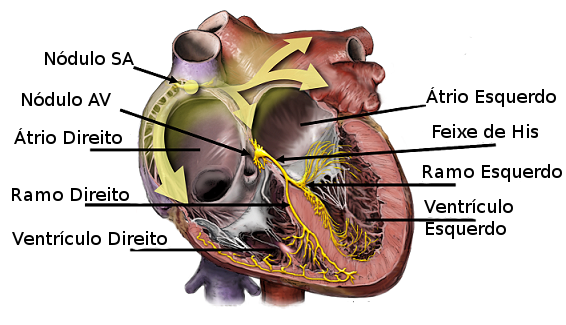
\includegraphics[width=400pt]{figures/chap2-heart.png}
    \caption[Coração e sentido da despolarização]{Coração e sentido da despolarização. Adaptada de \cite{blaufuss}.}
    \label{fig:heart}
\end{figure}

\section{Aquisição do eletrocardiograma}
O ECG é um exame médico que registra a atividade elétrica do coração. As fases do ciclo cardíaco são captadas por um eletrocardiógrafo com o auxílio de eletrodos (ou sensores) cutâneos. Os eletrodos são colocados aos pares no corpo do paciente, de forma que cada configuração de posicionamento dos eletrodos representa uma \textbf{derivação}. Um ECG padrão possui doze derivações, seis delas precordiais (tórax) e seis periféricas (membros). Uma derivação é formada por um eletrodo positivo e um eletrodo negativo, sendo que o ponto de contato do eletrodo positivo define a derivação utilizada.

Quando uma onda despolarização (cargas positivas) se move na direção de um eletrodo positivo instalado na pele do paciente, registra-se uma deflexão positiva no ECG. No caso de um sistema de aquisição com papel milimetrado, a ponteira do eletrocardiógrafo se moverá para cima no traçado. Num sistema de aquisição digital, as amplitudes do sinal na saída do conversor analógico-digital (A/D) se afastarão do valor de referência do conversor no sentido positivo.

Para obter as derivações periféricas, coloca-se eletrodos nos braço direito e esquerdo e na perna esquerda, disposição esta que forma um triângulo, como pode ser verificado a partir da figura \ref{fig:mleads}. A derivação I (DI) é composta por um par de eletrodos dispostos horizontalmente, com o pólo negativo colocado no braço direito e o positivo no braço esquerdo. Na derivação II (DII) o pólo negativo também é colocado no braço direito, porém o positivo vai na perna esquerda. E, finalmente, tem-se a derivação III (DIII) em que o pólo positivo vai na perna esquerda e o negativo no braço esquerdo.

\begin{figure}[ht!]
    \centering
    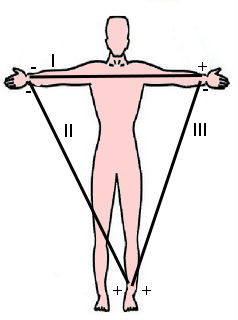
\includegraphics[width=150pt]{figures/chap2-mleads.png}
    \caption[Derivações periféricas: I, II e III]{Derivações periféricas: I, II e III.}
    \label{fig:mleads}
\end{figure}

As outras três derivações periféricas são as chamadas derivações aumentadas, quais sejam: aVR, aVF e aVL. A derivação aVR utiliza um eletrodo positivo no braço direito e um negativo comum (terra) dividido em três pontos de contato: um no braço esquerdo, um no pé esquerdo e outro no pé direito. A aVL é similar, porém com o pólo positivo no braço esquerdo e o negativo comum no braço direito, pé esquerdo e pé direito. Já a aVF é obtida com o pólo positivo no pé esquerdo e o negativo comum no braço esquerdo, braço direito e pé direito. Estas configurações podem ser visualizadas mais facilmente na figura \ref{fig:aleads}.

\begin{figure}[ht!]
 \centering
 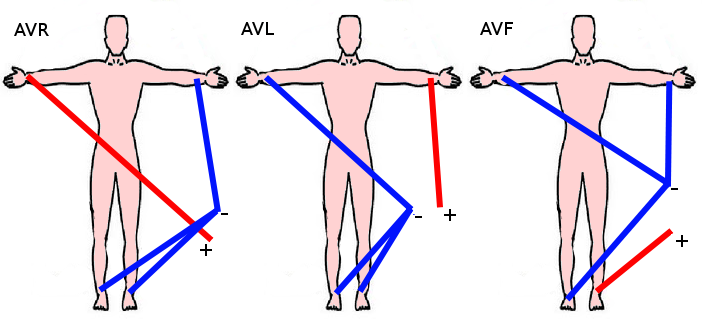
\includegraphics[width=400pt]{figures/chap2-aleads.png}
 \caption[Derivações periféricas aumentadas: aVR, aVL e aVF]{Derivações periféricas aumentadas: aVR, aVL e aVF.}
 \label{fig:aleads}
\end{figure}

As derivações precordiais ou torácicas são obtidas de maneira diferente. Coloca-se eletrodos positivos na parte frontal do tórax, conforme ilustrado na figura \ref{fig:vleads}. O dorso do paciente então é considerado como o pólo negativo da derivação. Na figura \ref{fig:aleads} é possível ver que as derivações V1 e V2 estão localizadas no lado direito do coração; V3 e V4 localizam-se sobre o septo interventricular; por fim, V5 e V6 ficam sobre o lado esquerdo do coração. O intuito dessas derivações é de cobrir totalmente o coração em sua posição dentro da caixa torácica.

\begin{figure}[ht!]
 \centering
 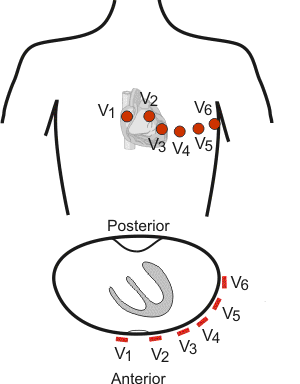
\includegraphics[width=150pt]{figures/chap2-vleads.png}
 \caption[Derivações precordiais: $V_1$, $V_2$, $V_3$, $V_4$, $V_5$ e $V_6$]{Derivações precordiais: $V_1$, $V_2$, $V_3$, $V_4$, $V_5$ e $V_6$. Extraída de \cite{Klabunde2008}}
 \label{fig:vleads}
\end{figure}

Na figura \ref{fig:beat} observa-se um batimento típico registrado em uma derivação de eletrocardiograma. Cinco ondas se distinguem na figura, denominadas pelas letras P, Q, R, S e T. A onda P representa a deflexão causada pela contração atrial (despolarização dos átrios). Já as ondas Q, R e S formam o chamado \textbf{complexo QRS} e representam a despolarização ventricular. Por último, a onda T representa a repolarização ventricular. A repolarização atrial, contudo, dificilmente pode ser visualizada no ECG porque se mistura com o complexo QRS.

\begin{figure}[ht!]
 \centering
 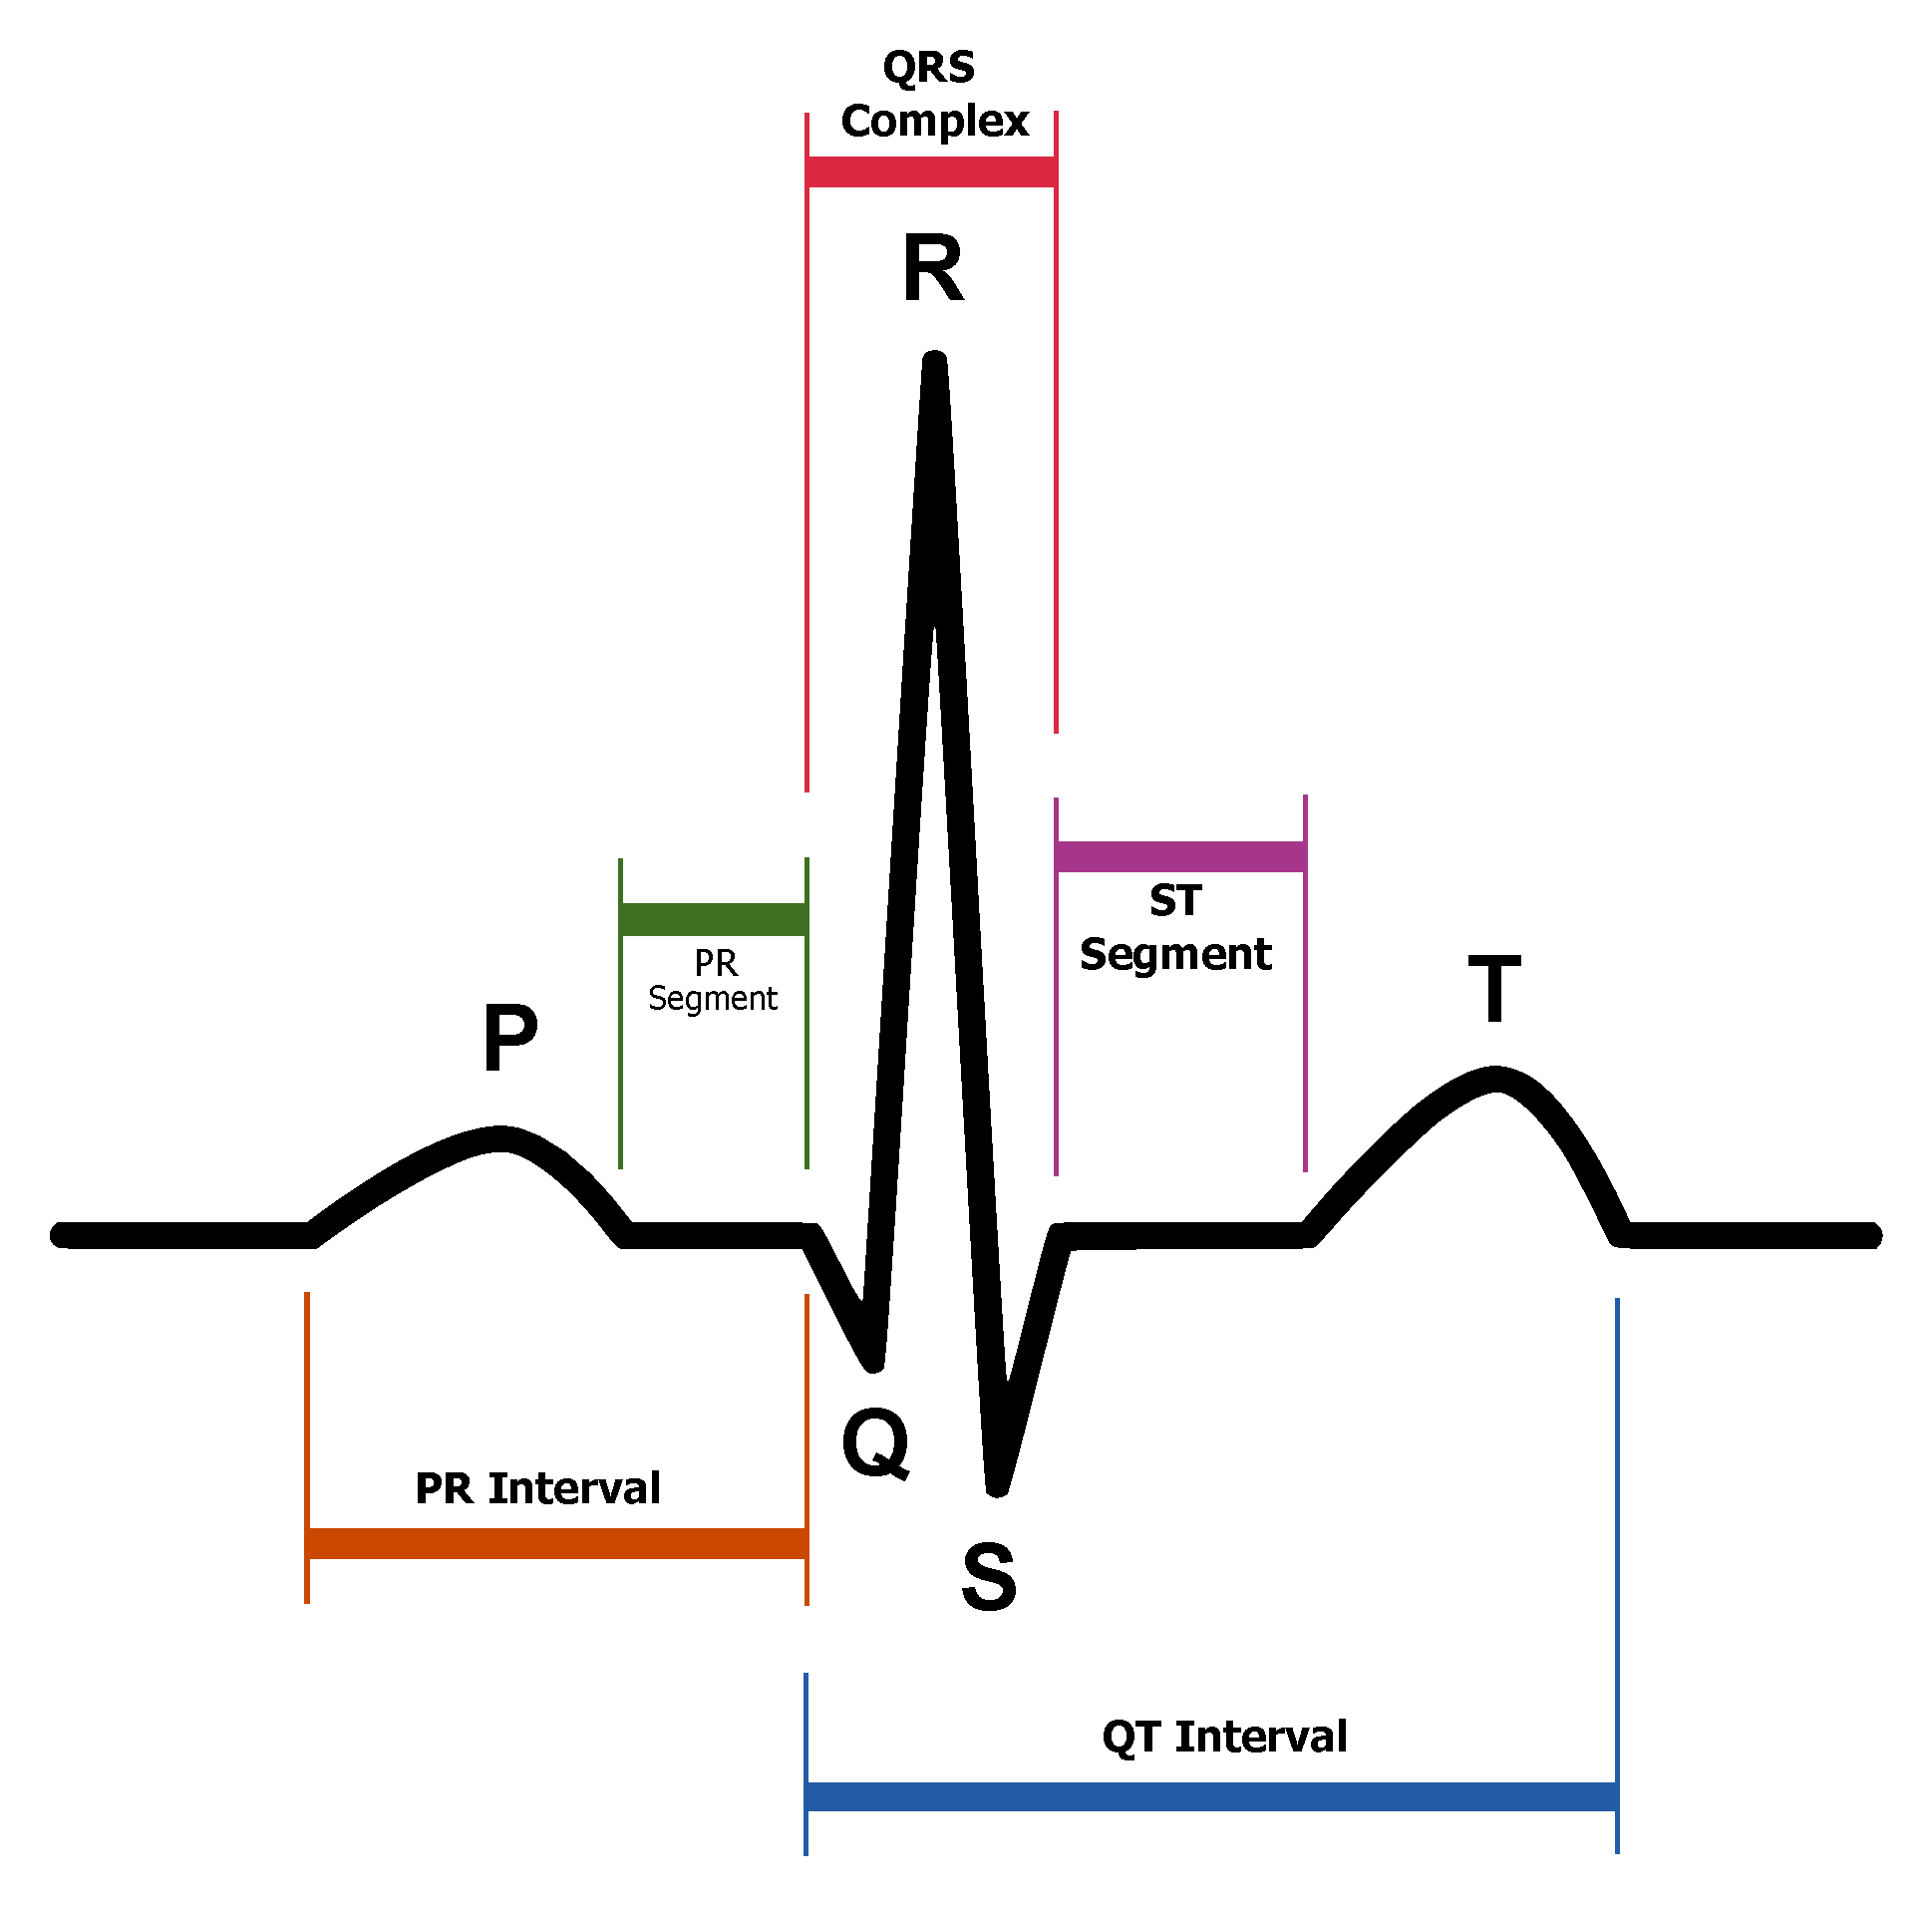
\includegraphics[width=300pt]{figures/chap2-beat.pdf}
 \caption[Ciclo cardíaco típico em um eletrocardiograma]{Ciclo cardíaco típico em um eletrocardiograma. Extraída de \cite{Atkielski2007}}
 \label{fig:beat}
\end{figure}

Ainda na figura \ref{fig:beat}, pode-se ver o chamado segmento PR, entre o fim da onda P e o início da onda Q, representando a pausa que existe entre a emissão do estímulo do Nódulo SA e o recebimento deste pelo Nódulo AV. O segmento ST, por sua vez, representa a pausa existente entre a contração ventricular e a repolarização ventricular. Há ainda o intervalo PR, que indica o tempo decorrido desde o início da despolarização atrial até o seu término. Finalmente, o intervalo QT indica o tempo entre o início da contração ventricular e o fim da repolarização ventricular.

\section{Interpretação do eletrocardiograma}
O ECG nos fornece informações valiosas a respeito da saúde física de um paciente. Em condições normais, um adulto apresenta morfologia de batimento cardíaco nos moldes da figura \ref{fig:beat}. Este padrão varia ligeiramente de acordo com a derivação escolhida, mas pode-se tomá-lo como referência na discussão que segue. Assim sendo, verá-se como uma doença cardíaca acarreta alterações no formato de ondas do ciclo cardíaco, quando analisado por meio do ECG. Ademais, informações como \textbf{frequência}, \textbf{ritmo}, \textbf{eixo}, \textbf{hipertrofia} e \textbf{infarto} podem ser avaliadas a partir do ECG. 

Determina-se a frequência com que os batimentos ocorrem pela distância entre os mesmos no eixo temporal; pode-se então avaliar o ritmo dos batimentos como uma medida qualitativa da variância da frequência cardíaca. Diz-se que o ritmo é normal se a frequência se mantém constante ou quase constante ao longo do intervalo de observação. Caso contrário, diz-se que o ritmo é irregular e tem-se então as chamadas arritmias.

A direção com que se propaga a onda de despolarização do coração é chamada de eixo e é representada por um vetor, o vetor do estímulo elétrico. A partir da análise de várias derivações em conjunto pode-se identificar o eixo, bem como possíveis anormalidades a seu respeito. Também a existência de hipertrofias cardíacas, ou seja, aumento da massa muscular do coração, pode ser observada. Finalmente, é possível averiguar ocorrência de infarto, isto é, morte parcial do músculo cardíaco resultante da oclusão de uma artéria coronária.

Os métodos estudados neste trabalho detectam apenas isquemia cardíaca. Para entender como a isquemia se manifesta no ECG, é necessário conhecer um pouco do sistema cardiovascular e saber que o coração recebe sangue pelas artérias coronárias (figura \ref{fig:arteries}). Quando, por algum motivo, um ramo da artéria coronária se estreita acentuadamente ou fica obstruído, a zona do miocárdio servida por esse ramo deixa de ter irrigação sanguínea adequada.

\begin{figure}[ht!]
 \centering
 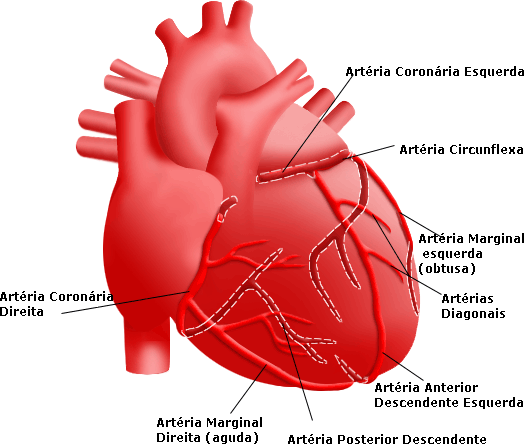
\includegraphics[width=300pt]{figures/chap2-arteries.png}
 \caption[Artérias coronárias]{Artérias coronárias. Extraído de \cite{yale}}
 \label{fig:arteries}
\end{figure}

O ventrículo esquerdo é a cavidade mais espessa do coração, necessitando portanto de maior quantidade de sangue. Assim, no caso de estreitamento das artérias coronárias, o ventrículo esquerdo é o primeiro a sofrer com a redução desse suprimento. É importante saber que o ventrículo esquerdo é em grande parte o responsável por enviar sangue para todas as partes do corpo. Quando parte do ventrículo esquerdo fica infartada, ela se torna eletricamente morta e não responde à despolarização. Consequentemente, ela não se contrai e acaba por prejudicar o bombeamento de sangue do coração. A figura \ref{fig:infarction} ilustra uma possível situação de infarto.

\begin{figure}[ht!]
 \centering
 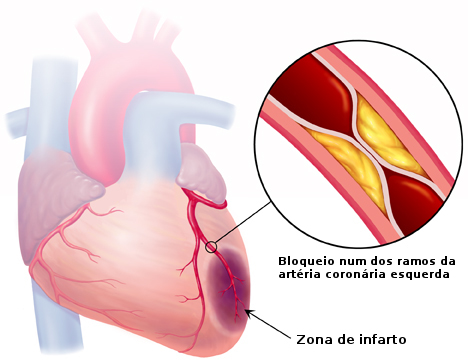
\includegraphics[width=300pt]{figures/chap2-infarction.jpg}
 \caption[Infarto do miocárdio]{Região de infarto do miocárdio. Extraído de \cite{Antipuesto2014}}
 \label{fig:infarction}
\end{figure}

A isquemia cardíaca é a redução do suprimento de sangue ou suprimento abaixo do normal. Ela precede um possível infarto e pode ser identificada no ECG principalmente através de duas características (ou uma das duas): inversão da onda T, podendo variar desde uma onda achatada ou deprimida até uma inversão profunda; e desnivelamento do segmento ST, podendo ser um supradesnivelamento ou um infradesnivelamento.

Nem toda diminuição do suprimento sanguíneo produz um infarto. Ondas T invertidas podem indicar a existência de isquemia sem infarto do miocárdio.  A onda T tipicamente isquêmica é simetricamente invertida. Como as derivações precordiais registram a atividade cardíaca em maior proximidade dos ventrículos, as alterações na onda T serão mais evidentes nessas derivações ($V_1$ a $V_6$). A figura \ref{fig:twave} mostra possíveis variações morfológicas da onda T.

\begin{figure}[ht!]
 \centering
 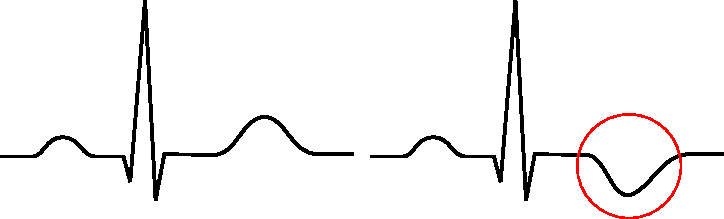
\includegraphics[width=400pt]{figures/chap2-t-waves.pdf}
 \caption[Onda T normal e Onda T isquêmica]{Onda T normal e Onda T isquêmica.}
 \label{fig:twave}
\end{figure}

A isquemia pode causar um lesão no tecido do miocárdio, caracterizando infarto agudo (recente). Para identificar a existência de lesão, analisa-se alteração no segmento ST. A elevação (supradesnivelamento) do segmento ST indica uma lesão e nos dá a certeza de que um infarto é agudo. Em certas situações, como Infarto Subendocárdico e Digitalis, o segmento ST apresenta uma depressão (infradesnivelamento). A figura \ref{fig:stdev} mostra as três variedades de nivelamento do segmento ST.

\begin{figure}[ht!]
 \centering
 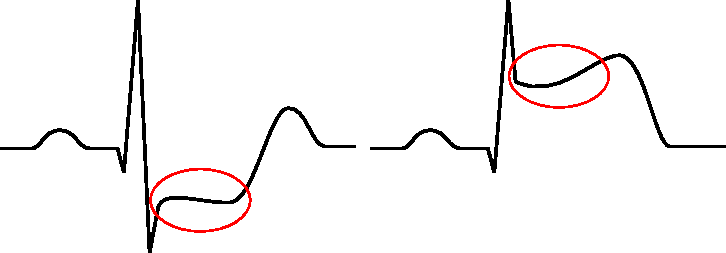
\includegraphics[width=400pt]{figures/chap2-st-segments.pdf}
 \caption[Segmento ST infradesnivelado e supradesnivelado]{Segmento ST infradesnivelado (1) e supradesnivelado (2).}
 \label{fig:stdev}
\end{figure}


\section{Resumo}
O ciclo cardíaco é um fenômeno fisiológico vital para os seres humanos. Essencialmente, tem-se que o Nódulo Sino-Atrial origina uma onda de despolarização (cargas positivas), consequente sístole atrial e, por meio do feixe de His, sístole ventricular. Após um período de repouso, átrios e ventrículos repolarizam-se (adquirem cargas negativas) e tornam-se capazes de iniciar um novo ciclo. É através desta atividade que o sangue circula em direção aos pulmões e para todo o resto do corpo, voltando ao coração após a troca gasosa e de nutrientes.

O exame de ECG registra as etapas do ciclo cardíaco por meio de derivações precordiais e/ou periféricas, formadas por um par de eletrodos cutâneos com cargas elétricas opostas. As derivações registram deflexões que representam cada uma das fases do ciclo, quais sejam: onda P, que é a deflexão causada pela contração atrial; as ondas Q, R e S, que formam o chamado complexo QRS e representam a contração ventricular; e a onda T, que representa a repolarização ventricular. A partir desse registro, é possível identificar informações como frequência cardíaca, ritmo, eixo, hipertrofia e infarto. 

Especialmente, estamos interessados em identificar isquemia cardíaca, que é a redução do suprimento de sangue ao coração. A falta de irrigação sanguínea adequada ao coração, sobretudo ao ventrículo esquerdo, antecede um possível infarto e pode ser identificada pela ocorrência de inversão da onda T ou desnivelamento do segmento ST. É com base nessas informações que se consegue diagnosticar a isquemia a partir do ECG.

% !TEX root = ../document.tex
% !TeX spellcheck = pt_BR

% ----------------------------------------------------------
\chapter[Noções de processamento de sinais]{Noções de processamento de sinais}
\thispagestyle{empty}
\label{chap:chapter3}
% ----------------------------------------------------------

Um pequeno ferramental matemático necessário para entender o tratamento de sinais digitais será apresentado neste capítulo. Num primeiro momento serão vistos conceitos como espaços, bases ortonormais e aproximação de vetores. Depois, a transformada de Fourier de tempo discreto e sua generalização, a transformada z, serão apresentadas. Em seguida, será feita uma breve discussão sobre a questão do projeto de filtros digitais. Por fim, serão discutidos os polinômios de Hermite e a expansão em funções de Hermite. Isto visa permitir um melhor entendimento dos próximos capítulos. Contudo, o leitor, se desejar, pode se referir apenas ao resumo no final do capítulo e prosseguir com a leitura do trabalho.


\section{Representação de sinais discretos}
\label{sec:discretesig}
Um sinal discreto $x[n]$ é uma sequência de valores em $\mathbb{R}$ ou $\mathbb{C}$, alocados em instantes de tempo discreto $n$. Normalmente, esta sequência representa as amplitudes geradas por um instrumento de medição sobre um processo físico qualquer, depois de amostradas e quantizadas por um conversor analógico-digital (A/D). Em particular, estamos interessados em processos reais (sem parte imaginária) e estocásticos, isto é, que não possuem comportamento previsível mas possuem propriedades estatísticas que os descrevem. Nas próximas subseções, verá-se como um sinal deste tipo pode ser decomposto em funções mais simples e conhecidas e também como se pode utilizar um conjunto finito e reduzido destas funções para aproximá-lo. Para um tratamento mais completo do assunto, sugere-se referir ao capítulo 2 do livro \cite{Vetterli1995}.

\subsection*{Espaços, bases e ortogonalidade}
Na álgebra linear, costumamos tratar espaços vetoriais de dimensões finitas, como $\mathbb{R}^n$ ou $\mathbb{C}^n$. Neste contexto, dado um conjunto de vetores ${v_k}$, desejamos responder a perguntas como:
\begin{itemize}
    \item o espaço em questão é \emph{gerado} (\emph{spanned}) pelo conjunto ${v_k}$? Em outras palavras, qualquer vetor no espaço pode ser representado por uma combinação linear de vetores de ${v_k}$?
    \item os vetores são linearmente independentes? Isto é, a afirmação de que um vetor em ${v_k}$ pode ser escrito como combinação linear dos demais é falsa?
    \item como é possível encontrar bases e, em particular, bases ortonormais, que geram o espaço?
    \item por fim, dado um subespaço e um vetor qualquer, como podemos encontrar uma aproximação para esse vetor no subespaço?
\end{itemize}

Para respondê-las, utilizamos as noções de \textbf{norma} (ou tamanho) e \textbf{ortogonalidade} de vetores. Dados dois vetores $x$ e $y$ no espaço $\mathbb{R}^n$, temos:
\begin{itemize}
    \item a norma quadrada: $\|x\| = \sqrt{\sum_{i=1}^{n} x^2_i}$
    \item o produto escalar: $\langle x,y \rangle = \sum_{i=1}^{n} x_iy_i$
    \item a propriedade de ortogonalidade: $\langle x,y \rangle = 0$
\end{itemize}

Quando se trabalha com espaços infinitamente dimensionais, fala-se de uma extensão da álgebra linear, que são os espaços de Hilbert. Um espaço de Hilbert é um espaço vetorial de dimensões possivelmente infinitas, equipado com um operador \textbf{produto interno}. Podemos escrever o produto interno $\langle\cdot,\cdot\rangle$ para o caso de sequências reais como:
\begin{equation}
    \langle x,y \rangle = \sum_{n=-\infty}^{\infty} x[n]y[n]
    \label{equ:innerprod}
\end{equation}

Este operador é linear, pois satisfaz as propriedades de aditividade $\langle x+y,z \rangle = \langle x,z \rangle + \langle y,z \rangle$ e homogeneidade $\langle x,\alpha y \rangle = \langle \alpha x,y \rangle = \alpha\langle x,y \rangle$, para $\alpha \in \mathbb{R}$. Também satisfaz $\langle x,x \rangle \geq 0$, e $\langle x,x \rangle = 0$ se $x=0$. Podemos usar o produto interno para definir normas e ortogonalidade. A norma de um vetor é escrita como $\|x\| = \sqrt{\langle x,x \rangle}$ e a distância entre dois vetores $x$ e $y$, como a norma de sua diferença $\|x-y\|$. Podemos ainda dizer que $x$ e $y$ são ortogonais, $x\perp y$, se $\langle x,y \rangle = 0$.

Precisamos também definir o conceito de base. Um subconjunto $S=\{x_1,\ldots,x_n\}$ de um espaço vetorial $E$ forma uma \textbf{base} para $E$ se o espaço é gerado por $S$ e se $x_i,\ldots,x_n$ são linearmente independentes. No caso de um espaço de dimensões infinitas, $S$ deve conter infinitos vetores linearmente independentes. Por exemplo, o conjunto $\{\delta[n-k]\}_{k\in\mathbb{Z}}$, em que $\delta[n]$ é a função impulso discreto unitário, forma uma base para o espaço de sequências infinitas, pois possui infinitos vetores linearmente independentes que geram este espaço.

Um caso especial é quando os vetores da base são ortogonais entre si e possuem norma unitária. Diz-se então que a base é ortonormal. O procedimento para se encontrar uma base ortonormal a partir de um conjunto de vetores linearmente independentes (que geram o espaço de interesse) é chamado de ortogonalização de Gram-Schmidt. Essencialmente, tem-se
\begin{equation}
    y_k = \frac{x_k-v_k}{\|x_k-v_k\|},
\end{equation}
onde $v_1 = 0$, e
\begin{equation}
    v_k = \sum_{i=1}^{k-1} \langle y_i,x_k\rangle y_i,\quad k=2,3,\ldots
\end{equation}
são as projeções sucessivas de um vetor do conjunto no subespaço gerado pelos vetores previamente ortogonalizados. Como será visto a seguir, esta expressão dá a melhor aproximação de um vetor no subespaço.


\subsection*{Aproximação por mínimos quadrados}

Dado um vetor $y$ num espaço $E$, deseja-se encontrar uma aproximação para este vetor que esteja num subespaço $S \subset E$. Assumindo que $S$ possua uma base ortonormal $\{x_1,x_2,\ldots\}$, a projeção ortogonal de $y \in E$ em $S$ é dada por
\begin{equation}
    \hat{y} = \sum_{i} \langle x_i,y\rangle x_i.
\end{equation}
A diferença $d=y-\hat{y}$ está no complemento ortogonal de $S$ e, em particular, $d$ é ortogonal a $\hat{y}$. Esta relação pode ser facilmente visualizada no espaço Euclideano tridimensional, conforme mostra a figura \ref{fig:three-dim}. Pela mesma figura, é possível ver que
\begin{equation}
    \|y\|^2 = \|\hat{y}\|^2+\|d\|^2.
\end{equation}
A aproximação é ótima no sentido de mínimos quadrados, isto é, o valor $min\|y-x\|$ para $x$ em $S$ e $y=\sum_{i} \alpha_ix_i$ é obtido com
\begin{equation}
    \alpha_i = \langle x_i,y\rangle.
\end{equation}
Os $\alpha_i$ são chamados coeficientes da expansão de $y$ em termos de $x_i$.

\begin{figure}[ht!]
    \centering
    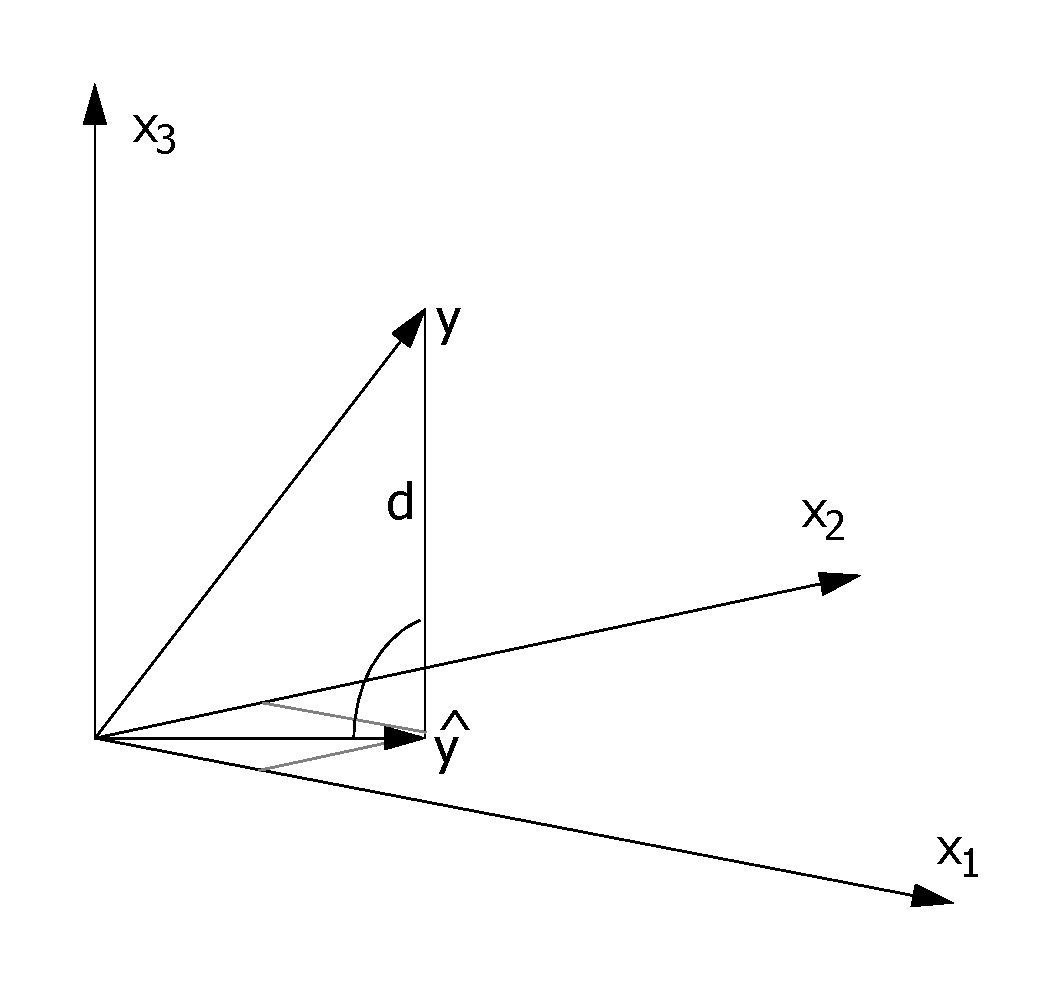
\includegraphics[width=200pt]{figures/chap3-three-dim.pdf}
    \caption[Projeção no espaço tridimensional]{Projeção no espaço tridimensional. Extraída de \cite{Vetterli1995}.}
    \label{fig:three-dim}
\end{figure}

A seguir será introduzida uma metodologia de representação de sinais discretos que usa como base a sequência de polinômios de Hermite. Esta técnica será utilizada em dois dos métodos de detecção de isquemia, conforme será visto nos capítulos \ref{chap:chapter5} e \ref{chap:chapter6}.

\subsection*{Polinômios de Hermite}
Os polinômios de Hermite podem ser obtidos pela seguinte relação de recorrência:
\begin{equation}
     \begin{array}{l}
         H_0(x) = 1\\
         H_1(x) = 2x\\
         H_{n+1}(x) = 2xH_n(x) - 2nH_{n-1}(x), \quad n \geq 1
     \end{array}.
\end{equation}
Ou podem ser expressos de forma explícita (não recursiva) por
\begin{equation}
     H_n(x) = n! \sum_{m=0}^{\lfloor \frac{n}{2} \rfloor} \frac{\left(-1\right)^m}{m!\left(n-2m\right)!}\left(2x\right)^{n-2m}.
\end{equation}
Os polinômios de Hermite são ortogonais entre si com respeito à função $e^{-x^2}$. Tomando o produto interno por esta métrica, tem-se:
\begin{equation}
     \int_{-\infty}^{\infty} H_m(x)H_n(x)e^{-x^2}dx = 0, \quad m\neq n
\end{equation}
Note aqui o uso da integral em vez do somatório (ver equação \ref{equ:innerprod}), por conta da variável $x$ ser contínua. Os primeiros seis polinômios de Hermite são descritos abaixo e têm seu gráfico mostrado na figura \ref{fig:hermpoly}.
\begin{equation}
     \begin{array}{l}
         H_0(x) = 1\\
         H_1(x) = 2x\\
         H_2(x) = 4x^2 - 2\\
         H_3(x) = 8x^3 - 12x\\
         H_4(x) = 16x^4 - 48x^2 + 12\\
         H_5(x) = 32x^5 - 160x^3 + 120x
     \end{array}
\end{equation}

\begin{figure}[ht!]
    \centering
    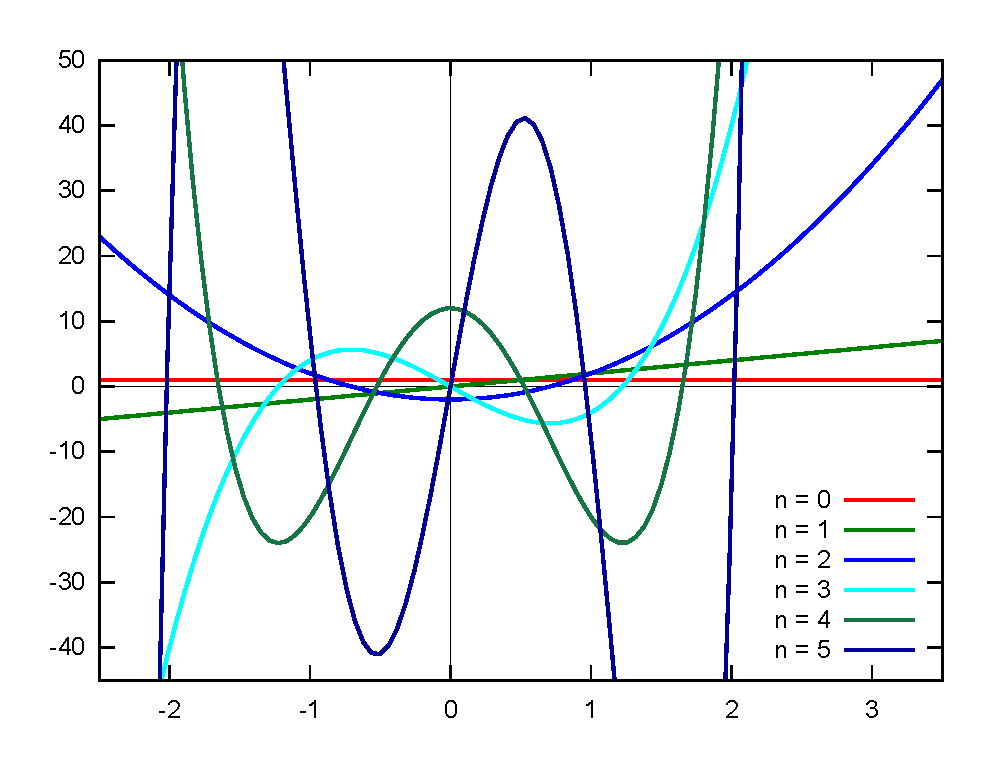
\includegraphics[width=300pt]{figures/chap3-herm-polynomials.pdf}
    \caption[Gráfico dos primeiros seis polinômios de Hermite]{Gráfico dos primeiros seis polinômios de Hermite. Extraído de \cite{Damato2009}.}
    \label{fig:hermpoly}
\end{figure}


\subsection*{Expansão em funções de Hermite}
As funções de Hermite são definidas em termos dos polinômios de Hermite, de acordo com a equação \ref{equ:hermfunc} abaixo. A figura \ref{fig:hermfunc} mostra o gráfico das primeiras seis funções.
\begin{equation}
    \psi_n(x) = \left(\frac{e^{-x^2}}{n!2^n\sqrt{\pi}}\right)^\frac{1}{2} H_n\left(x\right)
    \label{equ:hermfunc}
\end{equation}
De acordo com a teoria descrita em \cite{Abramowitz1974}, seguindo também o raciocínio introduzido para os polinômios de Hermite, essas funções são ortogonais entre si. Tomando o produto interno, tem-se:
\begin{equation}
     \int_{-\infty}^{\infty} \psi_m(x)\psi_n(x)dx = 0, \quad m\neq n.
\end{equation}
As funções de Hermite formam uma base ortonormal para o espaço de funções integráveis ao quadrado, $L^2(\mathbb{R})$. Portanto, têm aplicação direta na expansão de sinais desse tipo.

\begin{figure}[ht!]
    \centering
    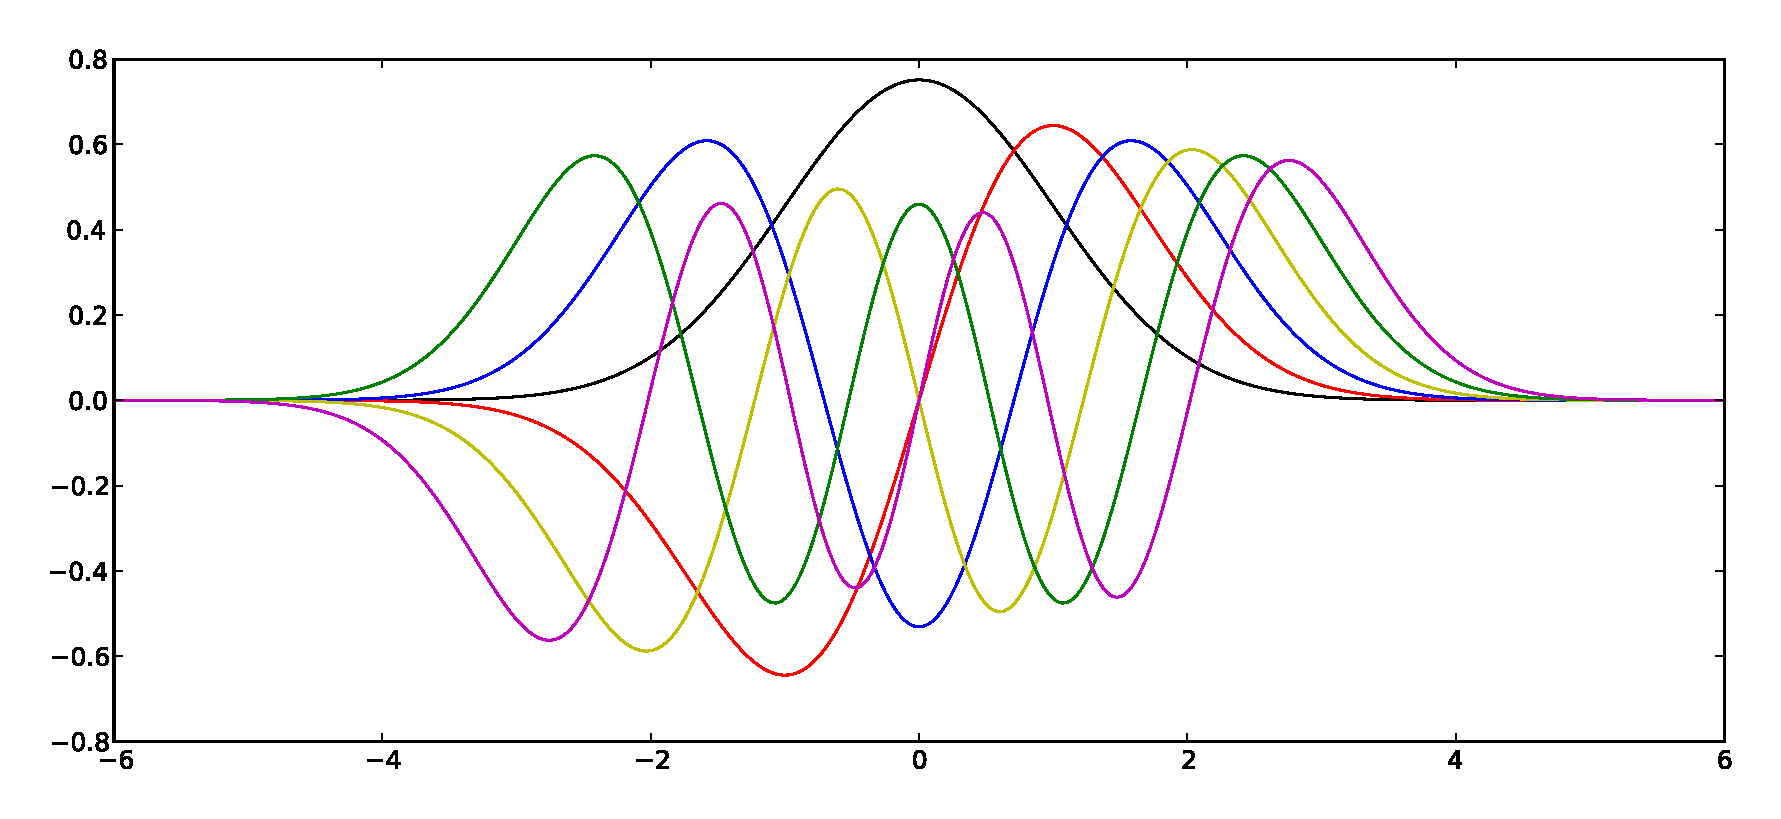
\includegraphics[width=400pt]{figures/chap3-herm-functions.pdf}
    \caption[Gráfico das primeiras seis funções de Hermite]{Gráfico das primeiras seis funções de Hermite. Extraído de \cite{Dems2009}.}
    \label{fig:hermfunc}
\end{figure}

No caso discreto, precisamos adotar uma abordagem um tanto diferente de cálculo dessas funções, que advém do fato delas serem autofunções da transformada de Fourier. Segundo a técnica descrita em \cite{Mugler2002}, as funções discretas de Hermite são autovetores de uma matriz tridiagonal e simétrica $T_b$. Esta matriz é completamente especificada por sua diagonal principal e diagonal secundária, cujos elementos são dados por
\begin{equation}
    d_{0,i} = -2\cos(N\pi\tau)\sin(i\pi\tau)\sin((N-i-1)\pi\tau), \quad 0\leq i\leq N-1
    \label{equ:maindiag}
\end{equation}
e
\begin{equation}
    d_{1,k} = \sin(k\pi\tau)\sin((N-k)\pi\tau), \quad 1\leq k\leq N-1,
    \label{equ:offdiag}
\end{equation}
onde $\tau = \frac{1}{Nb^2}$, $b$ é um parâmetro de dilatação e $N$ é o tamanho do sinal. O efeito do parâmetro $b$ é um alargamento das funções de Hermite no eixo temporal, à medida que $b$ aumenta.

Os autores advogam que o maior autovalor da matriz $T_b$ (num ordenamento do maior para o menor), corresponde à primeira função discreta de Hermite; o segundo maior autovalor, à segunda função de Hermite e assim por diante. Logo, o algoritmo de cálculo das funções discretas de Hermite consiste em construir a matriz $T_b$ conforme as equações \ref{equ:maindiag} e \ref{equ:offdiag}, extrair-lhe os autovetores e autovalores e, finalmente, enumerar os autovetores de acordo com seus respectivos autovalores em ordem decrescente. Uma vez normalizados (norma unitária), estes vetores formam uma base ortonormal para o espaço de sequências somáveis ao quadrado, $L^2(\mathbb{Z})$.

A expansão de $x[n]$, com $0\leq n\leq N-1$, por funções de Hermite se dá pelo produto interno de $x$ com cada um dos vetores previamente calculados. Podemos ainda construir uma matriz $U$ tendo esses vetores como linhas. Então a expansão se resume a um produto matricial $Ux$. Note que $x$, assim como $U$, possui dimensões finitas e, portanto, esta operação é na verdade uma aproximação. Em outras palavras, ela é a projeção de $x$ no subespaço gerado pelas linhas de $U$. A figura \ref{fig:hermexp} ilustra em linha pontilhada a aproximação de um sinal discreto (representado, por conveniência, usando linha contínua) usando as 50 primeiras funções discretas de Hermite.

\begin{figure}[ht!]
    \centering
    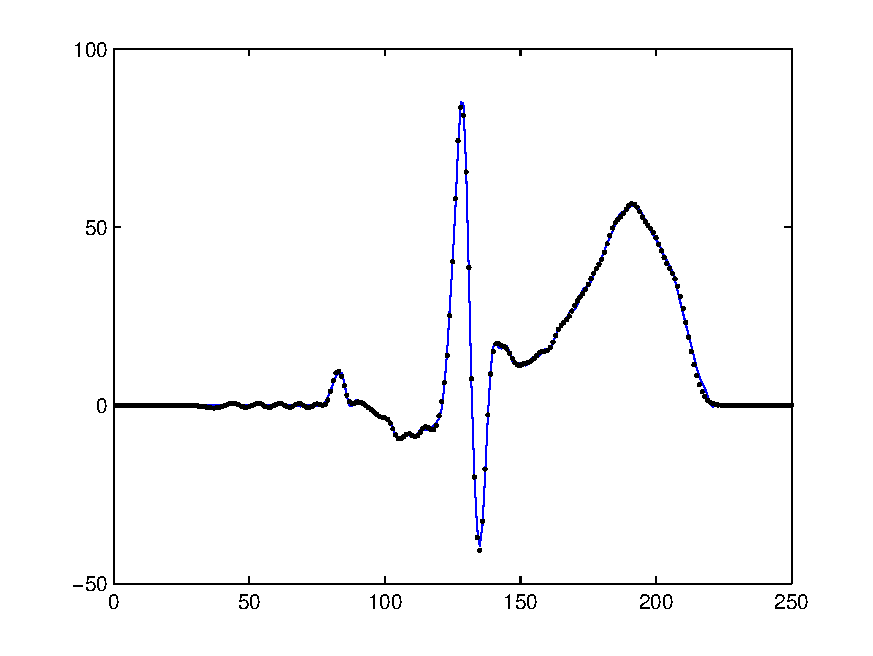
\includegraphics[width=400pt]{figures/chap3-herm-expansion.pdf}
    \caption[Gráfico da expansão usando 50 funções de Hermite]{Gráfico da expansão usando 50 funções de Hermite. Produzido no MATLAB.}
    \label{fig:hermexp}
\end{figure}


\section{Transformadas de tempo discreto}

A transformada de Fourier é uma ferramenta versátil de análise de sinais, pois evidencia componentes de frequência existentes num sinal e permite manipulá-lo por meio dessas componentes. Nesta subseção serão introduzidas a transformada de Fourier de tempo discreto e sua generalização, a transformada z. Ambas constituem o fundamento para a análise de sinais discretos no domínio frequencial, inclusive no que tange ao projeto de filtros digitais, assunto da seção consecutiva. A base para a discussão que segue, tanto nesta seção como na \ref{sec:filterdesign}, vem do livro \cite{Oppenheim2009}.

\subsection*{Transformada de Fourier de tempo discreto}
A transformada de Fourier de tempo discreto (DTFT) é definida como
\begin{equation}
     X(e^{j\omega}) = \sum_{n=-\infty}^{\infty} x[n]e^{-j\omega n}.
     \label{equ:dtft}
\end{equation}
Sua inversa, ou seja, a operação que fornece $x[n]$ a partir de $X(e^{j\omega})$ é
\begin{equation}
     x[n] = \frac{1}{2\pi}\int\limits_{(2\pi)} X(e^{j\omega})e^{j\omega n}.
\end{equation}

A equação \ref{equ:dtft} pode ser entendida como a relação que dá os coeficientes da expansão de $x[n]$ em funções exponenciais complexas, sendo estas as componentes de uma base para o espaço de sequências infinitas (e somáveis ao quadrado). A variável $\omega$ tem unidade em radianos.

\subsection*{Transformada z}

A transformada z é definida como
\begin{equation}
     X(z) = \sum_{n=-\infty}^{\infty} x[n]z^{-n},
\end{equation}
onde $z$ é, em geral, um número complexo: $z=Ae^{j\phi}$.

Por vezes, estamos interessados na representação de um sistema linear e invariante no tempo (LIT) através da transformada z, em cujo caso expressamos a equação de diferenças do sistema,
\begin{equation}
     \sum_{k=0}^{N} a_ky[n] = \sum_{k=0}^{M} b_kx[n],
\end{equation}
na forma (usando as propriedades de linearidade e deslocamento no tempo da transformada):
\begin{equation}
     Y(z)\sum_{k=0}^{N} a_kz^{-k} = X(z)\sum_{k=0}^{M} b_kz^{-k}.
\end{equation}
Podemos ainda escrever a função de transferência (ou resposta em frequência) do sistema como
\begin{equation}
     H(z) = \frac{Y(z)}{X(z)} = \frac{\sum_{k=0}^{M} b_kz^{-k}}{\sum_{k=0}^{N} a_kz^{-k}}.
     \label{equ:zresp}
\end{equation}

A equação \ref{equ:zresp} também pode ser rearranjada para evidenciar as raízes do polinômio numerador e do polinômio denominador, chamadas de zeros e pólos, respectivamente. Os zeros e pólos indicam os pontos onde a resposta em frequência do sistema cai a zero ou tende ao infinito. Eles são mais facilmente visualizados no \textbf{plano z}, conforme mostra a figura \ref{fig:zplane}. O plano z é uma ferramenta indispensável na análise de estabilidade e causalidade de sistemas discretos, bem como no projeto de filtros digitais, conforme será discutido na próxima seção.

\begin{figure}[ht!]
    \centering
    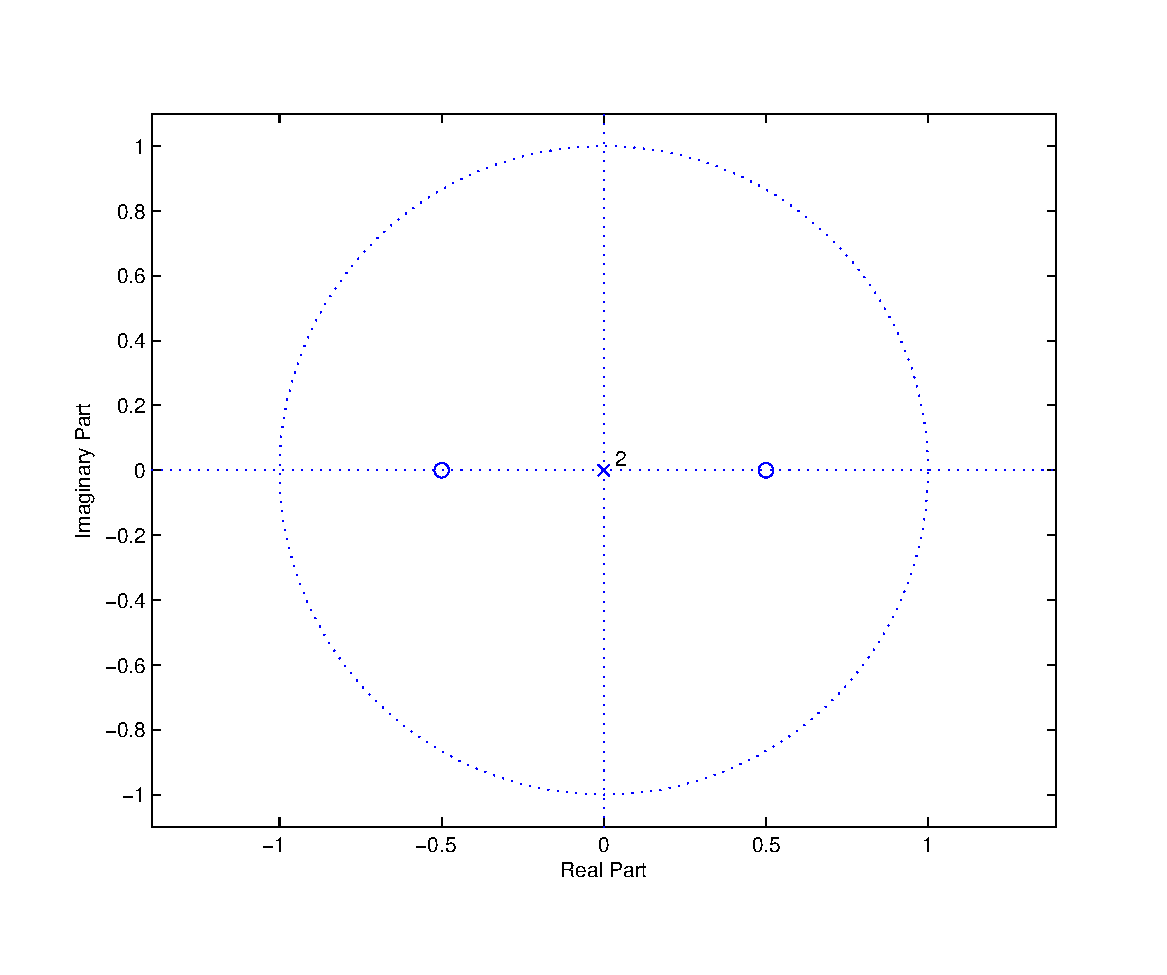
\includegraphics[width=300pt]{figures/chap3-z-plane.pdf}
    \caption[Plano z]{Plano z. Pólos duplos em $z=0$ e zeros em $z=\pm 0.5$.}
    \label{fig:zplane}
\end{figure}


\section{Projeto de filtros digitais}
\label{sec:filterdesign}
Filtros digitais têm uma grande variedade de aplicações, tanto na área biomédica quanto em qualquer outra que requeira processamento de sinais digitais. Neste trabalho, deseja-se manipular um sinal de ECG com vistas à detecção de batimentos cardíacos e também filtrá-lo para remover ruído e interferência da rede elétrica (50 ou 60 Hz). Esta seção apresenta alguns conceitos sobre o projeto de filtros digitais que auxiliarão o leitor no entendimento dos próximos capítulos, sobretudo no que tange à etapa de pré-processamento dos métodos de detecção de isquemia.

\subsection*{Tipos de filtros}
Há duas categorias básicas de filtros: o de resposta impulsiva finita (FIR) e o de resposta impulsiva infinita (IIR). O primeiro diz respeito àqueles filtros cuja resposta depende apenas da entrada em diferentes instantes de tempo. Em outras palavras, a equação de diferenças que descreve o comportamento do filtro não possui termos em $y[n-k], k\neq 0$. Isto também equivale a dizer que $H(z)$, a função de transferência do filtro, não possui pólos que não estejam localizados na origem do plano complexo z. A figura \ref{fig:firfilter} mostra a estrutura genérica de um filtro FIR.

\begin{figure}[ht!]
    \centering
    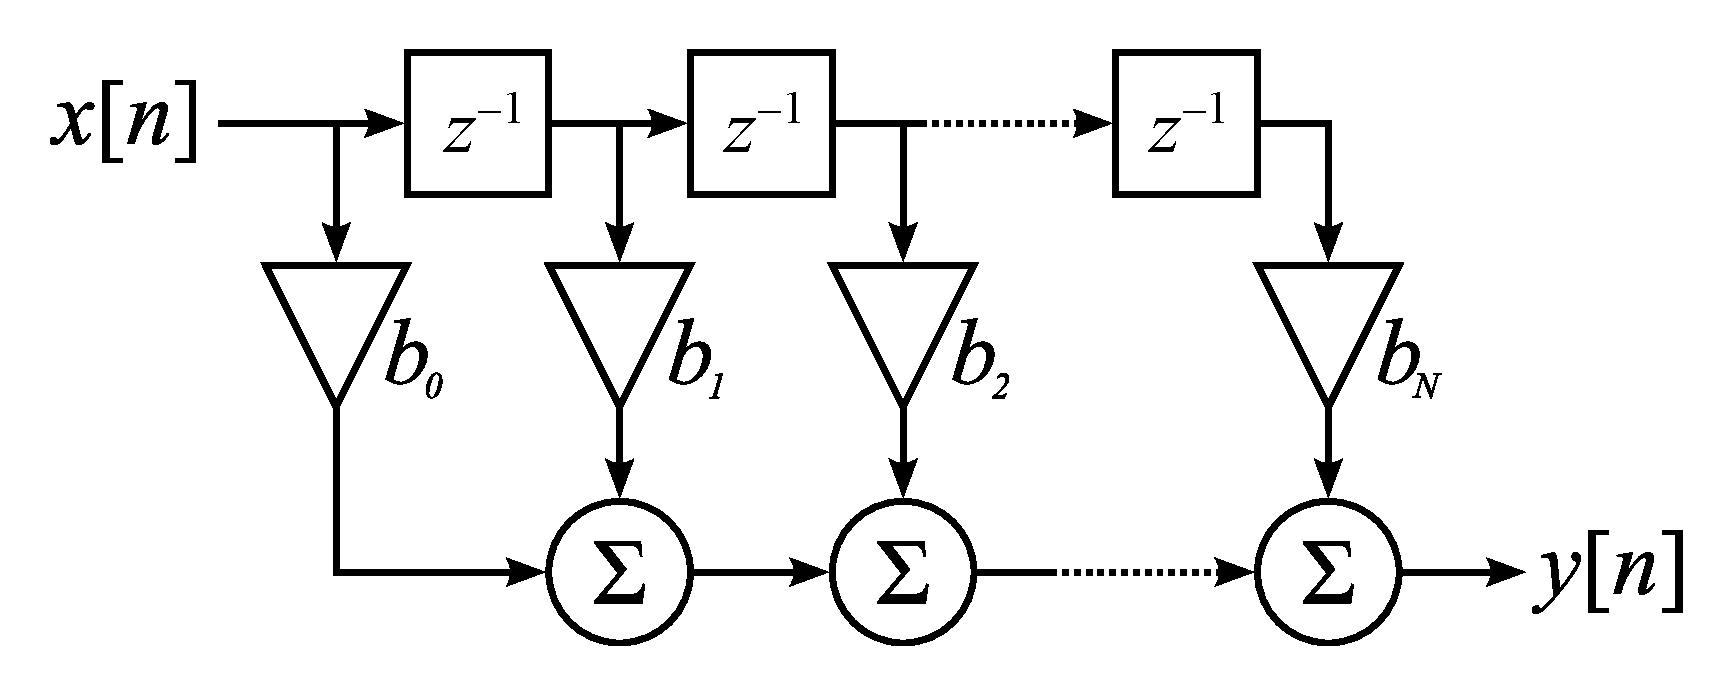
\includegraphics[width=300pt]{figures/chap3-fir-filter.pdf}
    \caption[Estrutura genérica de um filtro FIR]{Estrutura genérica de um filtro FIR. Extraída de \cite{Blanchard2008}.}
    \label{fig:firfilter}
\end{figure}

O segundo tipo de filtro diz respeito àqueles cuja resposta depende não apenas dos valores da entrada mas também dos valores da própria saída. Em outras palavras, há um laço de \emph{feedback} que conecta a saída a uma parte da entrada do filtro, realimentando-o. Isto implica dizer que sua resposta ao impulso será potencialmente infinita. Por esse motivo aliás, o filtro pode ser instável no sentido BIBO (\emph{bounded input, bounded output}), isto é, pode ter saída de valor ilimitado para uma entrada de valor limitado. A figura \ref{fig:iirfilter} mostra a estrutura genérica de um filtro IIR.

\begin{figure}[ht!]
    \centering
    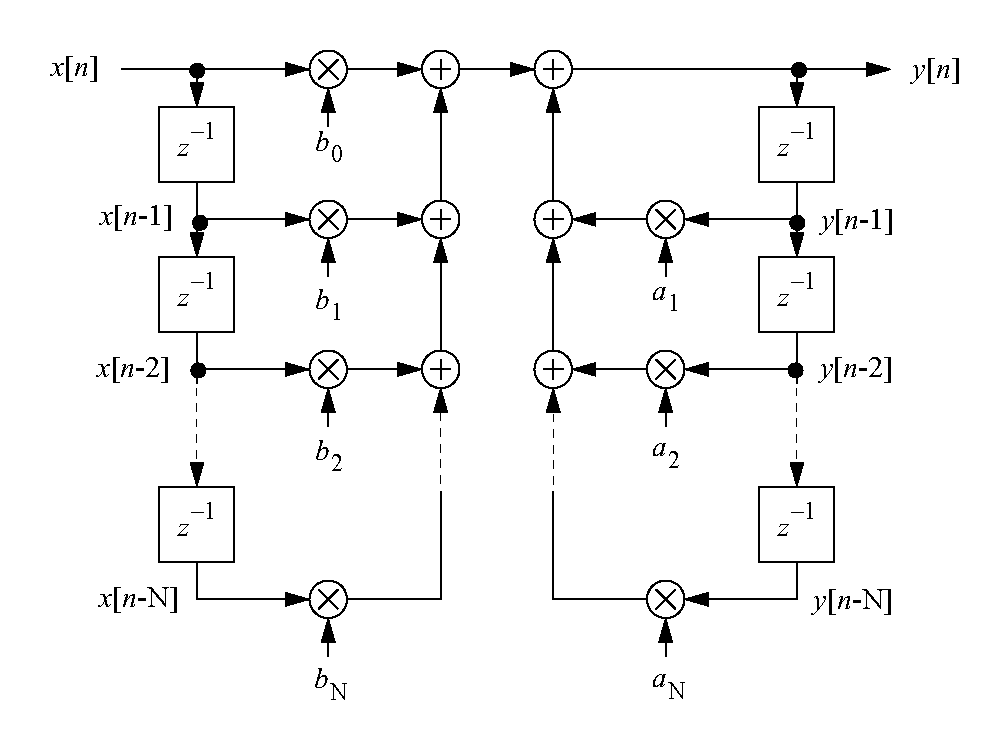
\includegraphics[width=400pt]{figures/chap3-iir-filter.pdf}
    \caption[Estrutura genérica de um filtro IIR]{Estrutura genérica de um filtro IIR.}
    \label{fig:iirfilter}
\end{figure}

Não se pretende aqui discutir em detalhe os critérios de estabilidade e causalidade de um filtro, questões estas que estão diretamente relacionadas com a região de convergência escolhida para a transformada z do sistema. Entretanto, vale mencionar que um filtro será realizável se ele for causal (saída zero para tempos menores que zero) e estável (saída limitada para entrada limitada). Todos os filtros projetados neste trabalho são realizáveis, de modo que podemos nos concentrar no projeto em si e não abordar estes princípios explicitamente.

Filtros FIR podem ser projetados de várias maneiras, sendo algumas delas: truncagem da resposta ideal, alocação de zeros no plano z e amostragem em frequência. Num primeiro momento, apresentaremos uma metodologia especial desenvolvida por Lynn (\cite{Lynn1971}, \cite{Lynn1977}), em que são projetados filtros com coeficientes inteiros. Consecutivamente, será vista a técnica de truncagem da resposta ideal por janelas. Esta última é necessária para o algoritmo de reamostragem que será visto no capítulo \ref{chap:chapter6}. Ao final da seção, será abordada questão de projeto de filtros IIR, necessária para o condicionamento do sinal de ECG (remoção de ruido/interferência).

\subsection*{Projeto de filtros FIR com coeficientes inteiros}
Lynn \cite{Lynn1977} propõe uma técnica de projeto de filtros FIR que proporciona vantagens sobre outras técnicas em termos de eficiência computacional, embora seja um tanto restritiva em termos de qualidade da resposta desejada. A principal vantagem desses filtros é que sua equação de diferenças possui apenas coeficientes inteiros, de modo que a filtragem possa ser realizada por multiplicações e adições inteiras, em vez de por operação em ponto-flutuante. Dependendo do caso, pode-se até realizar as operações de multiplicação por meio de deslocamentos de bits, tornando a filtragem ainda mais rápida.

A função de transferência base para um filtro passa-baixas nesta técnica é da seguinte forma:
\begin{equation}
     H_{lp}(z) = \frac{1-z^{-m}}{1-z^{-1}}.
     \label{equ:intlp}
\end{equation}
O termo denominador indica que há um pólo em $z=1$ (ou frequência $\omega =0$ rad), enquanto o termo numerador indica que existem $m$ zeros uniformemente distribuídos ao longo do círculo unitário, com ângulo de separação igual a $(2\pi/m)$ radianos. O zero em $z=1$ cancela o pólo no mesmo local, de modo que o filtro possui comportamento FIR. Não obstante, o pólo em $z=1$ introduz um termo em $y[n-1]$ na equação de diferenças, o que é claramente uma característica de filtros IIR. Esta também é uma vantagem, pois normalmente a equação de diferenças da versão IIR de um filtro FIR, quando ela existe, possui menos termos e, por consequência, necessita de menos operações (isto faz sentido porque o laço de realimentação reduz a dependência explícita da saída em termos da entrada).

A primeira coluna da figura \ref{fig:zeros} ilustra a disposição de zeros da equação \ref{equ:intlp} no plano z para alguns valores de $m$. Como o zero em $z=1$ é cancelado pelo pólo coincidente, a resposta em frequência do filtro tem seu pico neste ponto, em vez de cair a zero. A figura \ref{fig:freqzlp} mostra o módulo de $H_{lp}(z)$ quando $m=3$. A escala de frequências está normalizada no intervalo 0 a 1, correspondendo a 0 e $\pi$ radianos. Nota-se que a frequência onde o módulo cai a zero é igual a $(2\pi/3)$, ou, na escala da figura, $0,\overline{6}$. Nota-se também que o ganho do filtro na banda passante é o próprio valor de $m$, neste caso igual a 3. Isto vale para qualquer filtro no formato da Eq. \ref{equ:intlp}.

\begin{figure}[ht!]
    \centering
    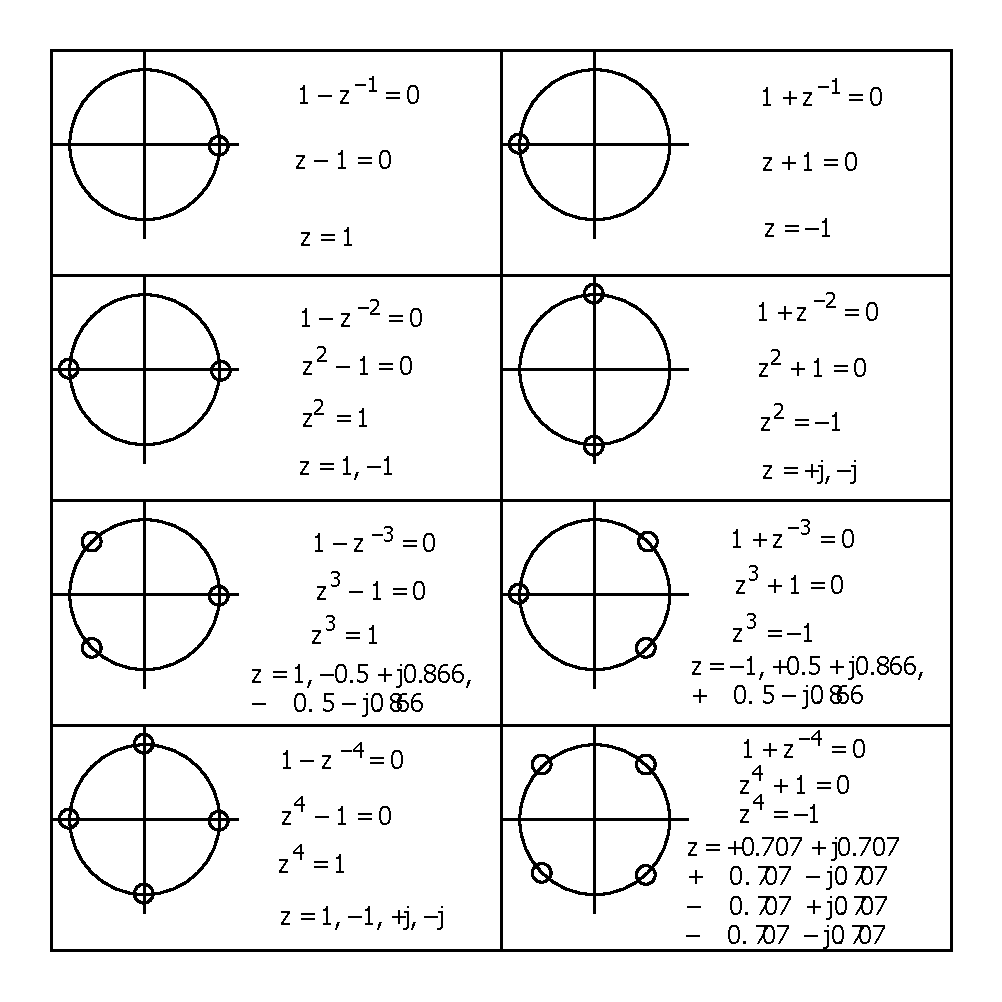
\includegraphics[width=400pt]{figures/chap3-zeros.pdf}
    \caption[Raízes de $1-z^{-m}$ e de $1+z^{-m}$]{Raízes de $1-z^{-m}$ (primeira coluna) e de $1+z^{-m}$ (segunda coluna). Extraída de \cite{Tompkins1993}}
    \label{fig:zeros}
\end{figure}

\begin{figure}[ht!]
    \centering
    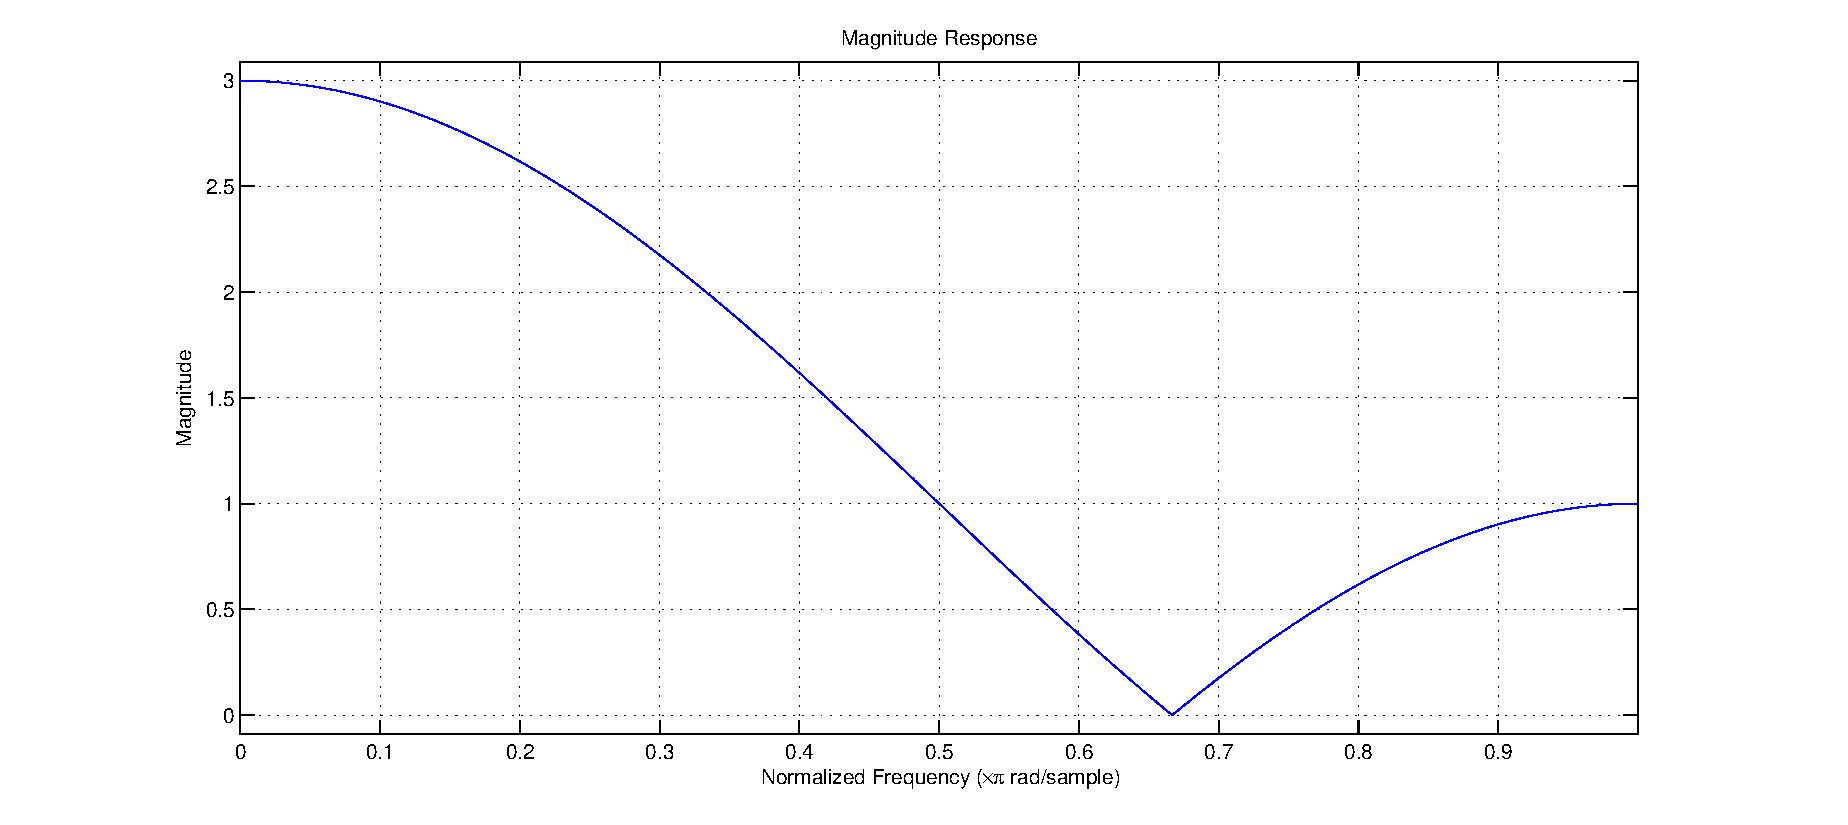
\includegraphics[width=500pt]{figures/chap3-freqz-lp.pdf}
    \caption[Resposta em frequência do filtro passa-baixas para $m=3$]{Resposta em frequência do filtro passa-baixas para $m=3$. Produzida no MATLAB}
    \label{fig:freqzlp}
\end{figure}

A função de transferência do passa-altas é similar, mas apresenta duas formas:
\begin{equation}
     H_{hp_1}(z) = \frac{1-z^{-m}}{1+z^{-1}}, \quad \quad
     H_{hp_2}(z) = \frac{1+z^{-m}}{1+z^{-1}}.
     \label{equ:inthp}
\end{equation}
Aqui o denominador indica que o pólo está em $z=-1$ (ou frequência $\omega =\pi$ rad). Na segunda forma, o numerador implica uma rotação na disposição de zeros no círculo unitário, em relação à primeira forma, conforme ilustra a segunda coluna da figura \ref{fig:zeros}. Isto significa que, para $m$ par, deve-se usar $H_{hp_1}(z)$ no projeto do passa-altas e usar $H_{hp_2}(z)$ somente quando $m$ for ímpar. A figura \ref{fig:freqzhp} mostra o módulo de $H_{hp_2}(z)$ quando $m=3$.

\begin{figure}[ht!]
    \centering
    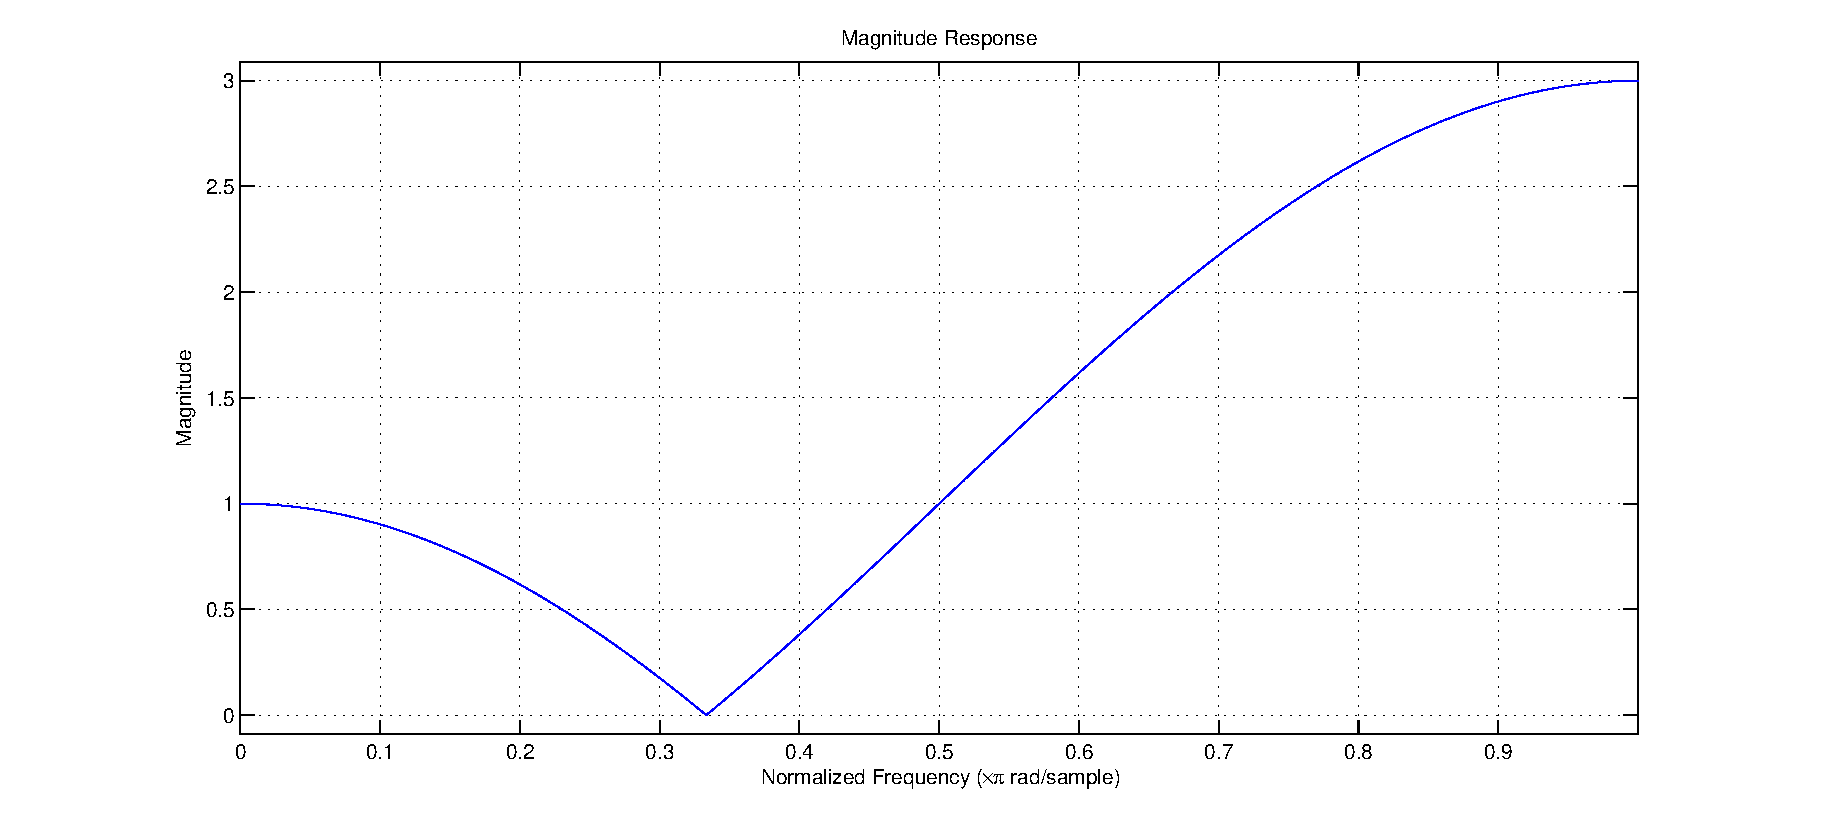
\includegraphics[width=500pt]{figures/chap3-freqz-hp.pdf}
    \caption[Resposta em frequência do filtro passa-altas para $m=3$]{Resposta em frequência do filtro passa-altas para $m=3$. Produzida no MATLAB}
    \label{fig:freqzhp}
\end{figure}

O parâmetro $m$ deve ser cuidadosamente escolhido para atender a uma determinada especificação. Nesta técnica de projeto, não há como satisfazer uma especificação arbitrária, pois a localização de pólos e zeros no círculo unitário é bastante restritiva. Contudo, dadas uma frequência de corte $\omega_c$ e a magnitude de $H(e^{j\omega})$ nesta frequência, é possível encontrar um valor de $m$ que atenda a essas restrições, mesmo que outras características da resposta em frequência permaneçam irrestritas. Assim sendo, deve-se resolver a equação
\begin{equation}
     \left.|H(e^{j\omega})|\right|_{\omega=\omega_c} = mC,
     \label{equ:solvem}
\end{equation}
onde $C$ é a magnitude desejada (com respeito a um ganho unitário) em $\omega_c$ e $m$ constitui o ganho do filtro na banda passante. De maneira similar, foi realizada a análise da função de transferência de ordem $N$, que nada mais é do que a composição de $N$ filtros iguais em cascata:
\begin{equation}
     H^N_{lp}(z) = \left(\frac{1-z^{-m}}{1-z^{-1}}\right)^N
\end{equation}
e
\begin{equation}
     H^N_{hp_1}(z) = \left(\frac{1-z^{-m}}{1+z^{-1}}\right)^N, \quad
     H^N_{hp_2}(z) = \left(\frac{1+z^{-m}}{1+z^{-1}}\right)^N.
\end{equation}

A equação \ref{equ:solvem} pode ser expressa como uma equação trigonométrica, usando a função seno, mas não possui solução analítica simples. Portanto, neste trabalho utilizou-se o resolvedor numérico do MATLAB (função \texttt{vpasolve}) e encontrou-se valores de $\omega_c$ para diversas combinações de $m$ e $C$. Variou-se $m$ no intervalo $[2,200]$ e $C$ possuía um de três valores, correspondendo às atenuações de -3dB, -6dB e -24dB, relativas ao ganho $m$ do filtro. A equação trigonométrica fornecida ao resolvedor vem da substituição $z=e^{j\omega}$ em $H^N_{lp}(z)$ e é dada por
\begin{equation}
     \left|\frac{\sin \left(m\frac{\omega}{2}\right)} {m\sin\left(\frac{\omega}{2}\right)}\right|^N = C.
\end{equation}
Com os valores de $m$ e $\omega_c$, para cada atenuação desejada e ordem $N$ do filtro, construiu-se um modelo de regressão que nos dá $m$ em função de $\omega_c$ e estimou-se os parâmetros do modelo usando a função \texttt{fitnlm} do MATLAB. Por fim, foi encontrado um modelo de regressão que expressa $m$ em função de $\omega_c$ e $N$, para $1\leq N \leq 10$. Abaixo estão as expressões encontrdas:
\begin{equation}
     m = \left\{
     \begin{array}{l l}
         \frac{0.91823\pi}{\omega_c\sqrt{N+0.072177}} & \quad \text{aten. de -3dB}\\
         \frac{1.2992\pi}{\omega_c\sqrt{N+0.15023}} & \quad \text{aten. de -6dB}\\
         \frac{1.732\pi}{\omega_c\sqrt{N+0.28356}} & \quad \text{aten. de -24dB}\\
         \frac{2\pi}{\omega_c} & \quad \text{aten. de $-\infty$}
     \end{array} \right..
\end{equation}

É importante ressaltar que o mesmo modelo pode ser usado tanto no projeto do passa-baixas quanto no do passa-altas, pois o que muda é a rotação da disposição de zeros no plano z e não o número de zeros que dividem o círculo unitário. (Podemos pensar no passa-altas como um deslocamento de $\pi$ radianos da resposta em frequência do passa-baixas.)

\subsection*{Projeto de filtros FIR por truncagem da resposta ideal}
A segunda maneira de projetar filtros FIR usada neste trabalho advém da construção da resposta impulsiva do filtro com base numa resposta ideal. A resposta em frequência de um filtro passa-baixas ideal é dada por:
\begin{equation}
     H_d(e^{j\omega}) = \left\{
     \begin{array}{l l}
         e^{j\omega\alpha} & \quad |\omega| \leq \omega_c\\
         0                 & \quad \omega_c \leq |\omega| \leq \pi
     \end{array} \right.,
\end{equation}
periódica com período $2\pi$. O parâmetro $\alpha$ é um fator de fase e garante, no domínio tempo, o atraso necessário para tornar o filtro causal. A figura \ref{fig:ideal} mostra um esboço da magnitude de $H_d(e^{j\omega})$. A resposta impulsiva do filtro é dada pela aplicação da transformada inversa de Fourier de tempo discreto:
\begin{equation}
     h_d[n] = \frac{1}{2\pi}\int_{-\omega_c}^{\omega_c} e^{j\omega\alpha}e^{j\omega n} = \frac{\sin \left( \omega_c \left(n-\alpha\right) \right)}{\pi \left(n-\alpha\right)}.
     \label{equ:impresp}
\end{equation}

\begin{figure}[ht!]
    \centering
    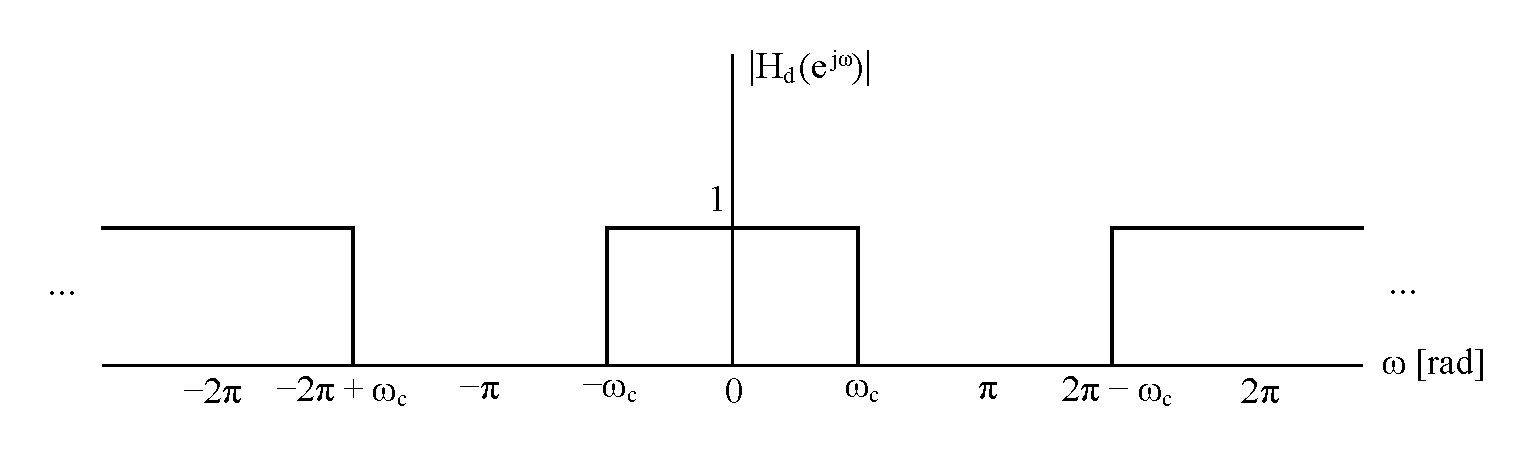
\includegraphics[width=400pt]{figures/chap3-ideal-lowpass.pdf}
    \caption[Resposta em frequência do filtro passa-baixas ideal]{Resposta em frequência do filtro passa-baixas ideal.}
    \label{fig:ideal}
\end{figure}

Desejamos truncar $h_d[n]$ num intervalo de tamanho $M$, com $\alpha=\frac{M}{2}$. Para tanto, utilizamos uma ``janela'' delimitadora, $w[n]$. Assim, tem-se
\begin{equation}
     h[n] = h_d[n]w[n], \quad 0\leq n \leq M,
     \label{equ:trunc}
\end{equation}
que no domínio frequência equivale a uma convolução de $H_d(e^{j\omega})$ com $W(e^{j\omega})$, e implica num ``espalhamento'' de energia da resposta ideal. A figura \ref{fig:design} mostra um esboço da magnitude de $H(e^{j\omega})$ juntamente com a resposta ideal (em traço segmentado). A figura também revela os diversos parâmetros utilizados no projeto do filtro.

\begin{figure}[ht!]
    \centering
    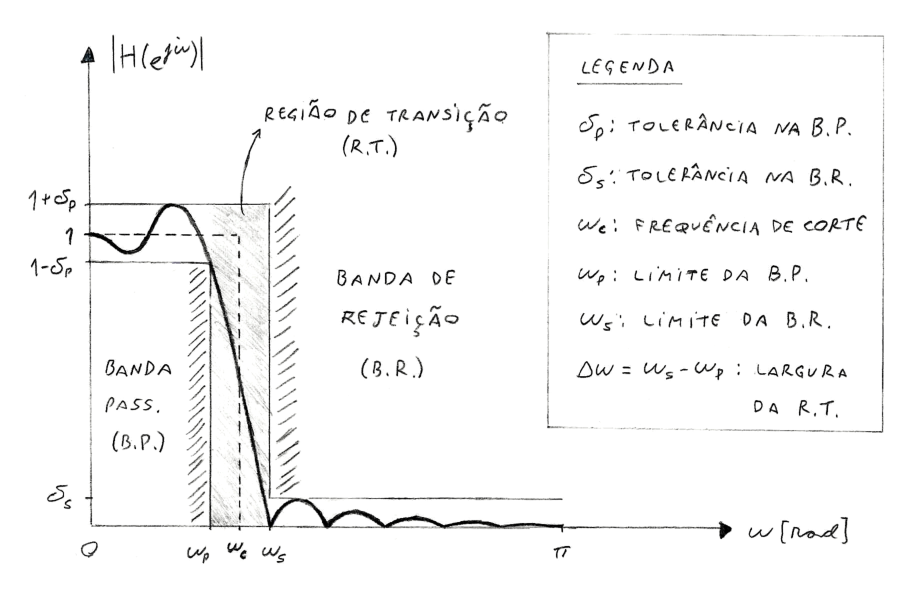
\includegraphics[width=350pt]{figures/chap3-design-lowpass.pdf}
    \caption[Especificações de projeto do filtro passa-baixas realizável]{Especificações de projeto do filtro passa-baixas realizável.}
    \label{fig:design}
\end{figure}

Visando reduzir o espalhamento de energia o tanto quanto possível, diversos tipos de janela foram propostos na literatura de processamento de sinais (\cite{Harris1978}, \cite{Kaiser1980}), cada uma com suas características. As características mais importantes de uma janela, do ponto de vista de sua resposta em frequência, são a largura do lóbulo principal e a atenuação média da banda de rejeição. Alguns tipos comuns de janela utilizados são: retangular, Bartlett (ou triangular), Hanning, Hamming, Blackman e Kaiser.

Os passos para se obter a resposta desejada de um filtro passa-baixas digital são:
\begin{enumerate}
    \item Tomar a menor tolerância entre as das bandas passante e de rejeição: $\delta = min(\delta_p,\delta_s)$;
    \item Calcular a atenuação requerida em decibéis, com base na tolerância: $A = -20\log_{10}(\delta)$;
    \item Escolher um tipo de janela que satisfaça a atenuação desejada; 
    \item Calcular a largura da região de transição: $\Delta\omega = |\omega_s-\omega_p|$;
    \item Descobrir o tamanho da resposta com base em $\Delta\omega$ e na janela: $M = f_w(\Delta\omega)$; e\footnote{a função $f_w$ é apenas uma maneira de dizer que existe uma relação entre $\Delta\omega$ e $M$}
    \item Calcular $h[n]$ usando as Eqs. \ref{equ:impresp} e \ref{equ:trunc}.
\end{enumerate}


\subsection*{Conversão de filtros IIR analógicos}
Historicamente, o projeto de filtros IIR digitais sempre teve como base as técnicas de projeto desenvolvidas no mundo contínuo, pois estas já são bastante avançadas e sofisticadas, de modo que é vantajoso reaproveitá-las no mundo discreto em vez de criar um novo ferramental ``a partir do zero''. A conversão da resposta impulsiva ou em frequência de um filtro de tempo contínuo para a resposta de um filtro de tempo discreto pode ser alcançada através de um dos seguintes procedimentos: invariância ao impulso (do inglês, \emph{impulse invariance}) ou transformação bilinear.

Abaixo está um condensado da segunda técnica supracitada, já que é a mais comumente utilizada em ferramentas computacionais de projeto de filtros, como o MATLAB. Na verdade, o que segue é apenas uma elucidação do procedimento de projeto. Diferentemente do caso FIR, em que se havia uma fórmula simples para obtenção da resposta do filtro, o projeto dos filtros IIR empregados neste trabalho será realizado com auxílio do MATLAB, conforme será visto no capítulo \ref{chap:chapter6}.

A transformação bilinear é dada pela substituição
\begin{equation}
     s = \frac{2}{T_d} \left(\frac{1-z^{-1}}{1+z^{-1}}\right),
     \label{equ:bilin}
\end{equation}
onde $T_d$ é um parâmetro associado à passagem do tempo contínuo para tempo discreto. Essa transformação mapeia o eixo $j\Omega$ do plano $s$ no círculo unitário do plano $z$. Isto é, mapeia $\Omega$ no intervalo $(-\infty,+\infty)$ para $\omega$ no intervalo $[-\pi,+\pi]$, sendo portanto não-linear. Por este fato, ela provoca uma distorção das frequências, conforme evidencia a relação
\begin{equation}
     \omega = \frac{2}{T_d} \arctan\left(\Omega \frac{T_d}{2}\right).
     \label{equ:warp}
\end{equation}

No projeto de um filtro IIR, é necessário converter as frequências especificadas ($\omega_p$ e $\omega_s$) no mundo digital para o seu correspondente contínuo, usando a Eq. \ref{equ:warp}. As tolerâncias ($\delta_p$ e $\delta_s$) não sofrem alteração. Com as especificações no mundo contínuo, determina-se a função de transferência do filtro analógico, que pode ser do tipo Butterworth, Chebyshev I, Chebyshev II ou elíptico, e finalmente faz-se a conversão da resposta para o mundo discreto usando a Eq. \ref{equ:bilin}.


\section{Resumo}
Este capítulo, que pode à primeira vista parecer extenso, assenta as peças necessárias ao entendimento dos assuntos vindouros. Aqui foram introduzidos os conceitos de norma, base e produto interno, no contexto de espaços vetoriais. Conceitos estes que dão lugar à questão da aproximação de sinais discretos. Uma interpretação foi apresentada no espaço Euclideano com auxílio da operação de projeção. Logo em seguida, viu-se que a sequência de polinômios de Hermite, assim como o conjunto de funções a ela associado, forma uma base ortonormal para o espaço de funções integráveis ao quadrado. No caso discreto, foi abordada uma técnica especial de cálculo das funções de Hermite que permite aproximação de um sinal discreto por meio de um simples produto matricial.

Depois, algumas transformadas de tempo discreto foram vistas, notadamente a transformada de Fourier de tempo discreto (DTFT) e a transformada z. Viu-se como é possível representar a equação de diferenças de um sitema linear e invariante no tempo (LIT) por meio da transformada z e que esta representação permite fácil identificação dos pólos e zeros do sistema. Ainda, o plano z oferece uma ferramenta imprescindível de análise de estabilidade e causalidade desses sistemas, bem como facilita o projeto de filtros, conforme visto na seção subsequente.

Existem diversas maneiras de se projetar filtros FIR, duas das quais foram discutidas na seção \ref{sec:filterdesign}. A primeira, tocante ao projeto de filtros com coeficientes inteiros, forneceu um algoritmo para determinação da função de transferência de filtros passa-baixa e passa-alta com coeficientes inteiros. Depois, foi visto o projeto de um filtro passa-baixa com base na truncagem de sua resposta ideal no domínio tempo. Essa truncagem se dá pelo uso de janelas delimitadoras e resulta em um algoritmo para o cálculo da resposta impulsiva do filtro. Ainda nesta seção teve lugar um breve discurso sobre a conversão de filtros IIR analógicos para o caso discreto, com ênfase na transformação bilinear.
% !TEX root = ../document.tex
% !TeX spellcheck = pt_BR

% ----------------------------------------------------------
\chapter[Avaliação de desempenho]{Avaliação de desempenho}
\thispagestyle{empty}
\label{chap:chapter4}
% ----------------------------------------------------------
A fim de avaliar os métodos de detecção de isquemia, necessita-se estabelecer métricas de avaliação. Interessa-se principalmente pela confiabilidade dos métodos, isto é, sua capacidade de classificar corretamente batimentos cardíacos em isquêmicos ou não isquêmicos. A seguir será apresentada a tradicional matriz confusão e dela serão derivadas seis métricas de avaliação de confiabilidade.

\section{Matriz de confusão}
Uma metodologia bastante popular de avaliação é por meio da \textbf{matriz de confusão}, um tipo especial de tabela de contingência\footnote{tabelas de contingência são usadas para registrar observações independentes de duas ou mais variáveis aleatórias.}. Ela separa os resultados de um teste diagnóstico em quatro categorias, que são as possíveis combinações de resultado positivo ou negativo no teste avaliado, com resultado positivo ou negativo num diagnóstico de referência, sendo este proveniente do conhecimento de especialistas. A tabela \ref{tab:confmatrix} mostra o formato geral da matriz de confusão.

\begin{table}[ht!]
    \centering
    \begin{tabular}{ccc}
    \toprule
    \multirow{2}{2cm}{Resultado do teste} &
    \multicolumn{2}{c}{Condição real} \\
    \cmidrule{2-3}
    & Presente & Ausente \\ 
    \midrule
    Positivo & verdadeiro positivo  & falso positivo \\
    & (VP) & (FP)\\
    \\
    Negativo & falso negativo & verdadeiro negativo \\
    & (FN) & (VN)\\
    \bottomrule
\end{tabular}
    \caption[Matriz de confusão para testes diagnósticos]{Matriz de confusão para testes diagnósticos.}
    \label{tab:confmatrix}
\end{table}

Para o trabalho desenvolvido, assim como para os métodos de detecção de isquemia originalmente propostos, o diagnóstico de referência está armazenado juntamente com os registros de ECG sob a forma de anotações. As anotações fornecem a localização dos batimentos cardíacos no tempo de gravação e dizem se um batimento foi considerado por cardiologistas como isquêmico ou não. Na verdade, as anotações referentes a isquemia estão organizadas de acordo com \textbf{episódios isquêmicos}. Os episódios têm início quando uma quantidade mínima de batimentos apresenta uma característica comum representando sintoma de isquemia e se estendem até o momento em que esta característica se torna ausente. Quatro tipos possíveis de característica sinalizam ocorrência de episódio isquêmico: elevação do segmento ST (denotada pelo símbolo ``ST+''), depressão do segmento ST (``ST-''), elevação da onda T (``T+'') e depressão da onda T (``T-'').

\section{Sensibilidade e Especificidade}
A sensibilidade é a capacidade do teste fornecer verdadeiros positivos (interpretação correta de ocorrência de isquemia) entre os batimentos verdadeiramente isquêmicos. Ela é obtida por
\begin{equation}
    SE = \dfrac{VP}{VP+FN}.
\end{equation}
No contexto de epidemiologia\footnote{epidemiologia é a ciência que estuda a distribuição de fenômenos patológicos e suas causas, nos seres humanos.}, sabe-se que um teste diagnóstico é sensível se ele raramente deixa de identificar indivíduos doentes. Este fato é importante na detecção de isquemia pois se deseja que, no melhor caso, todas as ocorrências de batimento isquêmico sejam identificadas.

A especificidade, por outro lado, é a capacidade do teste obter verdadeiros negativos (interpretação correta de ausência de isquemia) entre os batimentos verdadeiramente não isquêmicos. Ainda no contexto de epidemiologia, um teste é específico se ele raramente comete equívoco em identificar indivíduos sadios. A fórmula para o cálculo da especificidade é
\begin{equation}
    ES = \frac{VN}{VN+FP}.
\end{equation}

\section{Valores Preditivos Positivo e Negativo}
O valor preditivo positivo (também chamado de precisão ou preditividade positiva) é a razão entre os verdadeiros positivos e os diagnosticados como positivos pelo teste. Ele pode ser entendido como a probabilidade de um resultado positivo do teste refletir efetivamente a condição testada. Sua expressão é
\begin{equation}
    PP = \frac{VP}{VP+FP}.
\end{equation}
Em contrapartida, o valor preditivo negativo (ou preditividade negativa) é a proporção de verdadeiros negativos em relação aos diagnosticados como negativos pelo teste. Pode ser entendido como a probabilidade de um resultado negativo do teste refletir efetivamente a ausência da condição. Sua expressão é
\begin{equation}
    PN = \frac{VN}{VN+FN}.
\end{equation}

Os valores preditivos não se mantêm constantes para toda instância de teste realizada. Eles dependem da prevalência da doença na população. Se a prevalência for baixa, isto é, se relativamente poucos indivíduos se encontrarem doentes, obterá-se muitos falsos positivos, mesmo que o teste tenha especificidade alta. Reciprocamente, se a prevalência for alta, pode-se esperar um maior número de falsos negativos, ainda que o teste seja sensível. Portanto, quanto menor a prevalência, menor o PP e maior o PN, sendo a relação inversa também válida.

\section{Acurácia e Taxa de Falha}
A acurácia é a proporção de acertos na população e fornece uma medida do quão próximo o resultado do teste está do diagnóstico de referência. Ela é calculada por
\begin{equation}
    AC = \frac{VP+VN}{N}.
\end{equation}

A taxa de falha é a proporção de erros na população e fornece uma medida geral de falha do teste. Ela é dada por
\begin{equation}
    TF = \frac{FP+FN}{N}.
\end{equation}

% !TEX root = ../monografia.tex
% !TeX spellcheck = pt_BR

% ----------------------------------------------------------
\chapter[Métodos de detecção de isquemia]{Métodos de detecção de isquemia}
\thispagestyle{empty}
\label{chap:chapter5}
% ----------------------------------------------------------

Neste capítulo serão introduzidos os métodos de detecção de isquemia selecionados para implementação. Antes de detalhar cada método nas seções \ref{sec:rocha}, \ref{sec:mohebbi} e \ref{sec:gopalak}, far-se-á na seção \ref{sec:methods} uma pequena discussão sobre as possíveis categorias de métodos existentes. Ao final do capítulo, um breve resumo é apresentado contendo os aspectos principais dos métodos estudados.

\section{Categorização de métodos}
\label{sec:methods}
Na literatura, os métodos para detecção de isquemia, assim como para detecção de outros tipos de doença cardíaca, empregam técnicas variadas de (i) processamento de sinais, (ii) extração de características e (iii) classificação das características. Cada um destes grupos corresponde a uma etapa do processamento, sendo que todas incluem técnicas amplamente diversificadas.

O primeiro grupo constitui o que se denomina etapa de \textbf{pré-processamento}. A tabela \ref{tab:preprocessing} mostra algumas categorias de técnicas desta etapa e referências de algoritmos em cada categoria. A tabela \ref{tab:extraction} agrupa alguns métodos de detecção de acordo com técnicas usadas na \textbf{extração}, enquanto a tabela \ref{tab:classification} agrupa-os de acordo com técnicas usadas na \textbf{classificação}. Contudo, as técnicas de análise para extração e classificação não se limitam às das tabelas apresentadas. Há ainda métodos que utilizam modelagem paramétrica, mineração de dados, autômatos finitos, métodos sintáticos, entre outras. Também é importante mencionar que muitos dos algoritmos referenciados na primeira tabela são incluídos como parte da etapa de pré-processamento dos métodos de detecção de isquemia, que por sua vez são referenciados nas demais tabelas.

\begin{table}[ht!]
    \centering
    \begin{tabular}{p{140pt}p{280pt}}
    \toprule
    Filtragem linear (FIR/IIR, suavização, diferenciação, etc.) &
    \cite{Chen2006, Elgendi2013, Okada1979, Pan1985, Daskalov1998}\\
    Filtragem adaptativa &
    \cite{Park1998}\\
    Interpolação polinomial &
    \cite{Badilini1991}\\
    Técnicas não-lineares (matemática morfológica, produtório, máximo/mínimo, etc.) &
    \cite{Chu1989, Okada1979, Sun2005, Suppappola1994, Trahanias1993, Pan1985}\\
    Decomposição wavelet &
    \cite{Chen2006, Park1998}\\
    Thresholding adaptativo &
    \cite{Chen2006, Elgendi2013, Sun2005, Pan1985}\\
    \bottomrule
\end{tabular}
    \caption[Categorias de métodos de acordo com as técnicas de pré-processamento]{Categorias de métodos de acordo com técnicas comuns de pré-processamento.}
    \label{tab:preprocessing}
\end{table}

\begin{table}[ht!]
    \centering
    \begin{tabular}{p{140pt}p{280pt}}
    \toprule
    Uso de template &
    \cite{Akselrod1987, Garcia2000, Couceiro2008, Mohebbi2007}\\
    Decomposição wavelet &
    \cite{Ranjith2003, Senhadji1995, Milosavljevic2006}\\
    Transform. ortogonal (PCA, Karhunen-Loève, Hermite) &
    \cite{Castells2007, Rocha2010, Afsar2007, Gopalakrishnan2004, Pang2005}\\
    Análise frequencial ou tempo-frequencial &
    \cite{Rocha2010, Senhadji1995, Badilini1992, Couceiro2008}\\
    Propriedades estatísticas (correlação, erro médio, etc.) &
    \cite{Ranjith2003, Badilini1992, Couceiro2008, Garcia2000}\\
    Conhecimento prévio &
    \cite{Elgendi2013, Papaloukas2000}\\
    Características pontuais (pontos J e isoelétrico, picos de ondas, desvio de segmento ST) &
    \cite{Akselrod1987, Goletsis2004, Papaloukas2000, Ranjith2003, Rocha2010, Senhadji1995, Vila1997, Badilini1992, Couceiro2008, Mohebbi2007}\\
    \bottomrule
\end{tabular}
    \caption[Categorias de métodos de acordo com as técnicas de extração]{Categorias de métodos de acordo com técnicas comuns de extração.}
    \label{tab:extraction}
\end{table}

\begin{table}[ht!]
    \centering
    \begin{tabular}{p{140pt}p{280pt}}
    \toprule
    Redes neurais artificiais &
    \cite{Papaloukas2001, Rocha2010, Afsar2007, Couceiro2008, Gopalakrishnan2004, Mohebbi2007, Pang2005, Stamkopoulos1997, Maglaveras1998}\\
    Fuzzy ou neuro-fuzzy &
    \cite{Exarchos2007, Vila1997}\\
    Conjunto de regras &
    \cite{Akselrod1987, Exarchos2006, Papaloukas2002}\\
    Clusterização &
    \cite{Badilini1992}\\
    Modelos de Markov &
    \cite{Andreao2004}\\
    Algoritmos genéticos &
    \cite{Goletsis2004}\\
    \bottomrule
\end{tabular}
    \caption[Categorias de métodos de acordo com as técnicas de classificação]{Categorias de métodos de acordo com técnicas comuns de classificação.}
    \label{tab:classification}
\end{table}


\section{Método de Rocha et al.}
\label{sec:rocha}
Este método é baseado em dois pontos-chave: (i) desvio do segmento ST com relação à linha de base e (ii) expansão do complexo QRS e da onda T em funções de Hermite. A figura \ref{fig:rochadiag} mostra o diagrama em blocos da estratégia adotada. As etapas do método são detalhadas a seguir.

\begin{figure}[ht]
    \centering
    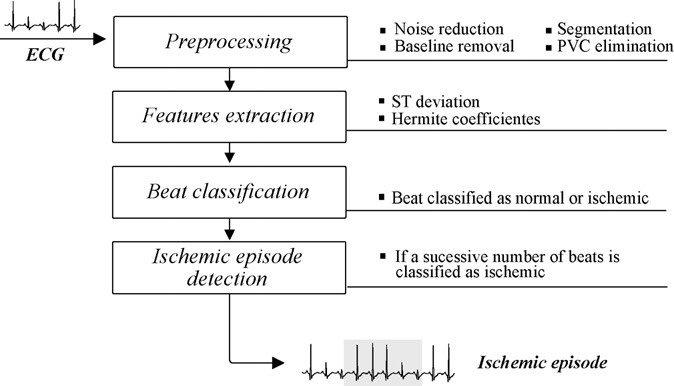
\includegraphics[width=300pt]{figures/chap5-rocha-diagram.png}
    \caption[Diagrama de blocos da estratégia utilizada no método de Rocha et al.]{Diagrama de blocos da estratégia proposta por Rocha et al. Extraído de \cite{Rocha2010}}
    \label{fig:rochadiag}
\end{figure}

\subsection*{Pré-processamento}
Nesta etapa, um sinal discreto contendo as amplitudes do ECG é processado com vistas à redução de ruído, segmentação em ondas características, eliminação de extra-sístoles ventriculares e, por último, remoção da linha de base.

A redução de ruído é realizada com um filtro passa-baixas de Butterworth de 4\textordfeminine{} ordem e frequência de corte 40 Hz. O sinal filtrado é então submetido a um procedimento de segmentação, em que as ondas características de cada batimento são identificadas. Na proposta dos autores, utiliza-se o algoritmo descrito em \cite{Sun2005}, baseado em derivação morfológica do sinal (um tipo de filtragem não linear, usando máximos e mínimos). Na saída obtêm-se as localizações de início, pico e fim de cada onda característica.

Após a segmentação, os batimentos passam por um procedimento de remoção de extra-sístole ventricular (ou PVC, do inglês \emph{premature ventricular contraction}), conforme descrito em \cite{Couceiro2008}. O último procedimento nesta etapa consiste em remover a linha de base em cada batimento cardíaco. Isto é necessário para as próximas etapas, onde se exige que os batimentos estejam bem alinhados com o nível isoelétrico do sinal.

\subsection*{Extração}
Nesta etapa, dois grupos de características são extraídos do ECG: (i) a medida do desvio de segmento ST e (ii) os coeficientes da expansão de Hermite do complexo QRS e das ondas T. Variações no desvio do segmento ST são usadas para discriminar os batimentos isquêmicos dos normais. De maneira similar, variações na morfologia do complexo QRS e da onda T indicam presença ou não de isquemia.

Para compor o primeiro grupo de características, dois valores são obtidos através de dois métodos distintos. Um deles é baseado na localização dos picos de onda R e na frequência cardíaca, conforme descrito em \cite{Pang2005}. O outro é derivado de uma análise do ECG em tempo-frequência, usando a transformada de Wigner-Ville descrita a seguir.

A distribuição de Wigner-Ville permite representar o espectro de frequências de um sinal contínuo ao longo do tempo. Ela é definida pela equação
\begin{equation}
    W_x(t,f) = \int_{-\infty}^{\infty} x\left( t+\frac{\tau}{2} \right) x^*\left( t-\frac{\tau}{2} \right) e^{-j2\pi f \tau} d\tau,
\end{equation}
onde o termo em $x$ é a função de autocorrelação instantânea e o operador $^*$ indica o conjugado complexo. Em tempo discreto, ela é chamada de pseudo-transformada de Wigner-Ville e assume a forma abaixo:
\begin{equation}
    W_x(nT,f) = 2T\sum_{p=-L_1}^{L_2} x[n+p]x^*[n-p]w[p]w^*[-p]e^{-j4\pi fp}.
    \label{equ:wigner}
\end{equation}

Nesta equação, $T$ é o período de amostragem e $w$ é uma janela simétrica de largura $L_1+L_2+1$. Os autores afirmam que o tamanho da janela deve ser maior que o do complexo QRS mais largo, para garantir que as características do formato de onda não sejam perdidas na transformação. Além disso, sabe-se que esta transformada pode ser calculada a partir da DFT (transformada discreta de Fourier) da autocorrelação de $x$ no tamanho da janela. Uma escolha conveniente para o tamanho da janela é uma potência de 2, pois neste caso o cálculo da DFT é mais eficiente. Por exemplo, assumindo que um complexo QRS não ultrapasse a largura de 100 ms e tomando uma frequência de amostragem de 250 Hz, pode-se utilizar uma janela de tamanho 32, pois $250\cdot 0,1 = 25$.

Após a transformação, soma-se os valores absolutos das componentes de baixa frequência do sinal em dois intervalos de tempo distintos: um à esquerda do pico de onda R e outro à direita do mesmo ponto. Os autores dizem utilizar os índices de frequência correspondentes a frequências entre 0 e 0,2 na escala normalizada. Entretanto, não mencionam quais os limites das faixas de tempo analisadas, nem mesmo o tipo de janela utilizado na Eq. \ref{equ:wigner}. Assume-se que a janela é do tipo retangular e que os limites das faixas de tempo devam ser estabelecidos conforme o caso.

O resultado da soma das componentes frequenciais provê informações sobre a concentração de energia nas duas faixas de tempo, sendo o restante do algoritmo uma simples busca pelo ponto mínimo em cada uma delas. O ponto mínimo à esquerda é o chamado ponto isoelétrico, enquanto o ponto mínimo à direita é chamado ponto J. Estes conceitos são discutidos em detalhe no artigo original. Basta apenas mencionar que a medida do desvio de segmento ST é a diferença entre as amplitudes nos pontos J e isoelétrico.

Para o segundo grupo de características, os autores propuseram uma técnica baseada na expansão em funções de Hermite. Já foi vista no capítulo \ref{chap:chapter3} a definição dessas funções em tempo contínuo para o caso particular em que elas não apresentam um parâmetro de dilatação. Aqui será reintroduzida a expressão da função de Hermite de tempo contínuo para o caso dilatado por um fator $l$, e usando a notação em $t$ da variável independente:
\begin{equation}
    \psi_n(t,l) = \left(\frac{e^{-(t/l)^2}}{n!2^n\sqrt{\pi}}\right)^\frac{1}{2} H_n\left(\frac{t}{l}\right)
\end{equation}

Pode-se perceber que aqui os autores optam por uma representação em tempo contínuo. A expansão consiste em obter uma lista de coeficientes que satisfazem a equação
\begin{equation}
   \hat{y}(t) = \sum_{j=0}^{M-1} c_j\psi_j(t,l),
\end{equation}
onde $c_j$ é o coeficiente da $j$-ésima função de Hermite e $M$ é o número de funções utilizadas na aproximação. Os coeficientes são dados pela solução algébrica do problema de minimização do erro quadrático, conforme a equação
\begin{equation}
    C = (H^TH)^{-1}H^TY,
\end{equation}
onde $C$ é um vetor coluna contendo os $M$ coeficientes da expansão, $Y$ é um vetor coluna contendo as amplitudes do sinal original e $H$ é uma matriz cujas colunas são as funções de Hermite:
\begin{equation}
    H = [\psi_0\ \psi_1\ \cdots\ \psi_{m-1}].
\end{equation}

Antes deste procedimento, contudo, o sinal de um batimento cardíaco é separado em dois segmentos: um deles contendo as amostras do complexo QRS e o outro, as da onda T. Essa separação permite aproximar melhor o formato do batimento em cada região, já que o complexo QRS e a onda T possuem morfologia distinta. Além disso, essas ondas estão bastante afastadas temporalmente, o que indica a necessidade de muitas funções de Hermite na aproximação caso se queira aproximar o sinal do batimento na íntegra. Os autores, pelo contrário, sugerem a utilização de apenas 6 funções na aproximação e, portanto, se justifica a separação em dois segmentos.

Os autores ainda mencionam a necessidade de reamostrar cada segmento para 64 amostras, afim de utilizar sempre a mesma largura para as funções de Hermite. Isto significa que a matriz $H$ pode ser calculada previamente e não se modifica durante a execução do algoritmo, permitindo aumento de eficiência na computação. Assim, dois conjuntos de 64 amostras por batimento são submetidos ao procedimento de expansão de Hermite, obtendo-se como resultado duas listas de 6 coeficientes. Estas listas são então incorporadas ao conjunto de características, de cuja parte já fazem as medidas do desvio de segmento ST.

\subsection*{Classificação}
O esquema de classificação usado por Rocha et al. envolve o uso de redes neurais artificiais. Para cada derivação de ECG, duas redes do tipo \emph{feed-forward} são treinadas com as características obtidas na etapa de extração. O algoritmo utilizado no treinamento é o Levenberg-Marquardt. O número de camadas é o mesmo para todas as derivações, sendo duas camadas ocultas mais a de entrada e a de saída. A função de transferência é a tangente sigmóide. O número de neurônios na entrada corresponde ao número de características extraídas, qual seja, $2+6+6=14$, enquanto a saída conterá apenas um neurônio, que fornece o resultado correspondente a elevação ou a depressão do segmento ST. O critério de inversão da onda T não é utilizado nesta estratégia. A figura \ref{fig:rochaclass} ilustra o esquema de classificação assim proposto.

\begin{figure}[ht]
    \centering
    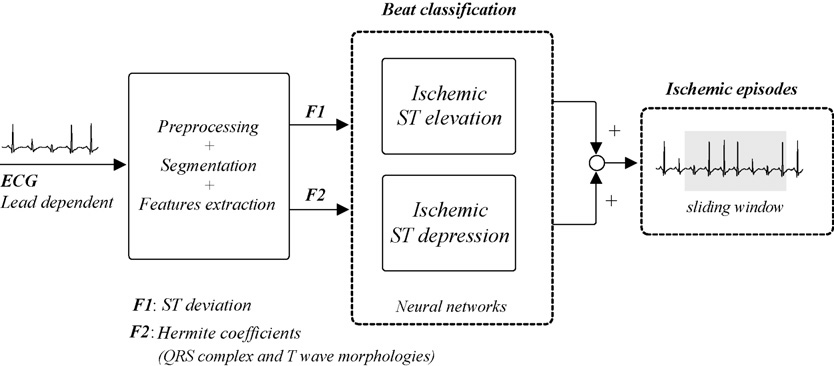
\includegraphics[width=400pt]{figures/chap5-rocha-class.png}
    \caption[Diagrama da estratégia de classificação de Rocha et al.]{Diagrama da estratégia de classificação de Rocha et al. Extraído de \cite{Rocha2010}}
    \label{fig:rochaclass}
\end{figure}

Ainda nesta etapa, há um procedimento de detecção de episódios isquêmicos. Sugerem os autores que um episódio isquêmico seja detectado toda vez que uma sequência de 40 batimentos tiver pelo menos metade classificada como isquêmica. Assim, uma janela de tamanho 40 percorre o resultado da classificação avançando um batimento por vez e sinaliza a ocorrência de um episódio quando o número de batimentos isquêmicos ultrapassa 20, ou sinaliza a ausência de episódio quando este número cai a 20 ou menos. Num segundo passo, episódios adjacentes com separação menor que 40 batimentos são unidos.


\section{Método de Mohebbi e Moghadam}
\label{sec:mohebbi}
Este método tem como principal recurso a obtenção de um modelo (ou \emph{template}, em inglês) de batimento cardíaco considerado normal, extraído do próprio registro sobre o qual se deseja fazer a detecção de isquemia. As etapas do algoritmo podem ser visualizadas no diagrama da figura \ref{fig:mohebbidiag} e seus detalhes são discutidos a seguir.

\begin{figure}[ht]
    \centering
    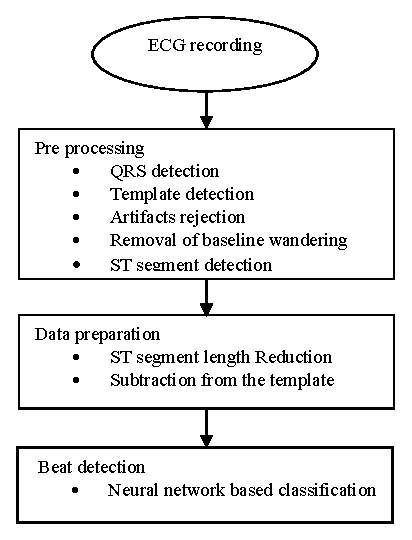
\includegraphics[width=250pt]{figures/chap5-mohebbi-diagram.pdf}
    \caption[Diagrama de blocos da estratégia proposta por Mohebbi e Moghadam]{Diagrama de blocos da estratégia proposta por Mohebbi e Moghadam. Extraído de \cite{Mohebbi2007}}
    \label{fig:mohebbidiag}
\end{figure}

\subsection*{Pré-processamento}
Esta etapa consiste de identificação dos complexos QRS, obtenção de um modelo de batimento, remoção de ruído, rejeição de artefatos e extração do segmento ST. A identificação dos complexos QRS e dos picos de onda R é feita através de um algoritmo descrito em \cite{Tompkins1993}, que faz uso extensivo de filtragem para realçar os complexos QRS e de \emph{thresholding} para a detecção. Na saída obtêm-se uma lista com as localizações dos picos de onda R.

Em seguida, os primeiros 30 segundos do registro de ECG são inspecionados afim de detectar artefatos ou batimentos considerados anômalos. Tal procedimento é feito através de uma estimativa do ponto isoelétrico e do ponto J de cada batimento. A estimativa se dá pela análise do gradiente do sinal. Caso nenhum dos dois pontos seja detectado, o batimento em questão é considerado como artefato e removido da lista. Os batimentos remanescentes são usados para construção do modelo, que é a média aritmética entre as amplitudes dos batimentos. Em seguida, o resto do sinal é processado e a linha de base é estimada através de interpolação \emph{spline} cúbica, segundo o método descrito em \cite{Badilini1991}.

\subsection*{Extração}
Na etapa de extração, detecta-se o ponto J de cada batimento usando novamente o gradiente do sinal. Neste caso, uma janela de 100 ms à direita do pico de onda R é suavizada por um filtro de média móvel. Em seguida, busca-se na janela o primeiro intervalo de 20 ms cujo declive médio seja menor que 2,5 mV/s em valor absoluto. Toma-se o ponto central deste intervalo como o ponto J. Obtidos os pontos J, assume-se que os segmentos ST iniciem neste ponto e possuam largura pré-definida de 160 ms. O mesmo se aplica ao batimento modelo, do qual se extrai o segmento ST usado como referência no algoritmo.

Os dados que constituem a entrada para a etapa de classificação são a diferença entre o segmento ST dos batimentos e o segmento ST de referência. Dada uma taxa de amostragem $f_s$, o segmento ST possui $\lfloor0.16f_s\rfloor$ amostras. Afim de reduzir o tamanho do conjunto de características, os sinais de segmento ST (inclusive o do modelo) são reamostrados para 20 amostras.

\subsection*{Classificação}
Mohebbi e Moghadam também fazem uso de redes neurais artificiais para a etapa de classificação. Aqui, uma única rede neural é treinada usando o algoritmo de \emph{backpropagation} com taxa de aprendizado adaptativa, combinado ainda com a técnica de treinamento com \emph{momentum}. Os autores justificam o uso dessas técnicas argumentando que o desempenho do \emph{backpropagation} é bastante sensível ao valor estabelecido para a taxa de aprendizagem, sendo que o valor ótimo deste parâmetro varia de acordo com a complexidade da superfície do erro. Dessa forma, uma taxa de aprendizado adaptativa se manterá no maior valor possível enquanto também permanece estável. O treinamento com \emph{momentum} significa que a rede responderá não apenas ao gradiente local, mas também a tendências recentes na superfície do erro.

A camada de entrada da rede possui 20 neurônios, que recebem a sequência de valores oriunda da etapa de extração. A rede possui uma camada oculta também com 20 neurônios. A camada de saída contém dois neurônios, cujo valor de saída está no intervalo real de 0 a 1. As saídas da rede neural são o grau de pertinência a cada uma das classes (presença ou ausência de isquemia), sendo que o máximo entre as duas designa a classificação final. O treinamento da rede se encerra quando a soma do erro quadrático for menor que 0,01 ou quando o número limite de 2000 épocas é atingido.


\section{Método de Gopalakrishnan et al.}
\label{sec:gopalak}

O terceiro e último método estudado faz uso de uma série de propriedades da álgebra linear e também da relação entre as funções discretas de Hermite e a matriz de Fourier\footnote{matriz de Fourier é aquela que, multiplicada por um vetor, resulta na DFT do vetor}. As etapas do algoritmo são ilustradas pelo diagrama da figura \ref{fig:gopalakdiag}, sendo detalhada a seguir.

\begin{figure}[ht]
    \centering
    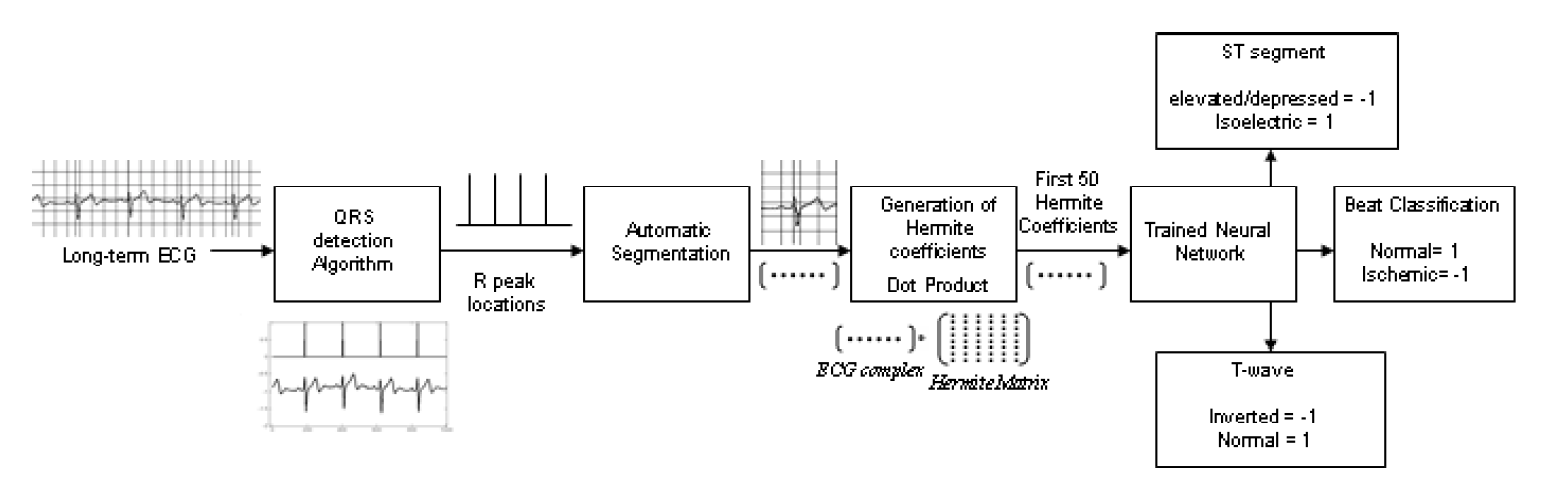
\includegraphics[width=1.0\textwidth]{figures/chap5-gopalak-diagram.png}
    \caption[Diagrama de blocos da estratégia adotada por Gopalakrishnan et al.]{Diagrama de blocos da estratégia adotada por Gopalakrishnan et al. Extraído de \cite{Gopalakrishnan2004}}
    \label{fig:gopalakdiag}
\end{figure}

\subsection*{Pré-processamento}
O método proposto não inclui nenhuma informação especial sobre procedimentos na etapa de pré-processamento, com exceção da própria detecção de batimentos cardíacos. Neste caso, os autores utilizam o mesmo algoritmo de detecção QRS mencionado para o caso do método anterior, qual seja, o algoritmo de Tompkins. Após obtenção dos picos de onda R, cada batimento deve ser centralizado neste ponto e sua largura é equivalente ao intervalo entre o seu pico e o do batimento vizinho (chamado intervalo R-R, ou apenas RR). Entretanto, técnicas como as de remoção da linha de base ou redução de ruído/interferência não estão presentes neste método.

\subsection*{Extração}
Para cada batimento, os primeiros 50 coeficientes de Hermite são extraídos, utilizando exatamente o mesmo ferramental introduzido no capítulo \ref{chap:chapter3}, no que diz respeito às funções discretas de Hermite. Estes coeficientes constituem, integralmente, o conjunto de características fornecido à etapa de classificação. Os autores ainda explicam, baseando-se em trabalhos passados e também pela observação do erro RMS (do inglês, \emph{root mean square}) percentual, que o uso de 50 coeficientes e de um parâmetro de dilatação $b=1$, garantem uma aproximação bastante boa.

\subsection*{Classificação}
Gopalakrishnan et al. utilizaram cinco redes neurais em seu esquema de classificação. A justificativa é que o resultado de redes individuais pode variar em casos limítrofes de isquemia. Desse modo, o resultado majoritário de um comitê de cinco redes fornece a decisão final sobre a classe a que pertence um batimento. As redes possuem três camadas ocultas com diferentes números de neurônios em cada uma. A camada de saída possui dois neurônios, que indicam presença ou não de alterações no segmento ST e presença ou não de inversão da onda T.

Os autores não especificam um algoritmo para o treinamento das redes. Contudo, relatam a realização de um procedimento adicional em cada registro de ECG de longa duração. Eles explicam que as redes são retreinadas usando alguns exemplares de ciclo cardíaco normal do ECG e argumentam que isso fornece às redes um ``toque'' das características normais de segmento ST e onda T daquele registro em particular.


\section{Resumo}
Neste capítulo foram apresentados os métodos de detecção de isquemia estudados no trabalho. Primeiramente, algumas categorias foram usadas para agrupar os métodos de acordo com as principais técnicas de detecção utilizadas.

Depois, foi visto em detalhe o método proposto por Rocha et al., que emprega um procedimento sofisticado de segmentação de batimentos e também várias técnicas para eliminação de ruído, linha de base e extra-sístoles ventriculares (PVCs). O método sugere a utilização de dois grupos de características: o do desvio de segmento ST e o dos coeficientes da expansão em funções de Hermite. Particularmente, este método faz uso de análise espectral dos batimentos para obtenção do ponto J. Na etapa de classificação, cada derivação tem uma rede neural treinada somente com características advindas daquela derivação. As características usadas no treinamento das redes são a elevação e a depressão do segmento ST.

O método de Mohebbi et al., embora um pouco menos sofisticado, também emprega diversas técnicas de pré-processamento para remover a linha de base, detectar os pontos J e isoelétrico e eliminar artefatos. Em especial, este método constrói um modelo de batimento cardíaco e de segmento ST, do qual se obtém a diferença com os demais segmentos ST extraídos. A etapa de classificação deste método é bastante simples, já que emprega apenas uma rede neural para todas as derivações. Aqui também são usadas a elevação e a depressão do segmento ST no treinamento.

Por fim, foi apresentado o método proposto por Gopalakrishnan et al. Este poderia ser considerado o mais simples dos três, já que não faz uso de nenhuma técnica especial na etapa de pré-processamento. Sua etapa de extração também é simples, pois se resume a um produto matricial correspondendo à expansão em funções discretas de Hermite. A etapa de classificação do método emprega cinco redes neurais, sem que haja distinção entre as derivações, e computa o resultado como a decisão majoritária das cinco redes. Todas as características indicativas de isquemia são usadas no treinamento das redes deste método.

% !TEX root = ../document.tex
% !TeX spellcheck = pt_BR

% ----------------------------------------------------------
\chapter[Projeto e Implementação]{Projeto e Implementação}
\thispagestyle{empty}
\label{chap:chapter6}
% ----------------------------------------------------------

Este capítulo descreve o projeto e a implementação dos métodos de detecção de isquemias cardíacas propostos por Rocha et al., por Mohebbi e Moghadam e por Gopalakrishnan et al.. Será abordado o projeto das três etapas dos métodos -- pré-processamento, extração e classificação -- assim como o projeto dos testes. Ao longo da discussão, será feito um relacionamento dos itens de projeto com a sua contra-parte na implementação (código-fonte). Ao final do capítulo será apresentado uma síntese sobre o projeto. O objetivo aqui é definir e mostrar como foi construído o ferramental utilizado para obtenção dos resultados práticos. Este trabalho foi realizado em cooperação com Guilherme Lazarotto de Lima, Mestrando em Computação pela UFRGS.

\section{Projeto do pré-processamento}
Como foi discutido no capítulo \ref{chap:chapter5}, cada método emprega técnicas variadas de pré-processamento do sinal de ECG. Não obstante essa diversidade, dois deles utilizam algum tipo de condicionamento do sinal (eliminação de ruído, linha de base, etc.) e todos se utilizam de algum algoritmo de detecção e segmentação de batimentos cardíacos. Um deles, o de Mohebbi e Moghadam, ainda emprega uma técnica de remoção de artefatos com base num \emph{template}. Outro, o de Rocha et al., usa um procedimento de remoção de PVCs, adaptado de \cite{Couceiro2008}.

No início do projeto, fez-se uma tentativa de implementar cada método de detecção separadamente, cada qual utilizando suas técnicas, conforme proposto nos artigos originais. Contudo, essa abordagem se mostrou ineficaz e propícia a erros de implementação. Ineficaz porque há redundância de informações que são obtidas na etapa de pré-processamento, como filtragem do sinal para redução de ruído e interferências, remoção da linha de base, detecção de batimentos e delimitação das ondas do ciclo cardíaco. Propícia a erros de implementação porque cada técnica tem como base um algoritmo proposto em um artigo científico diferente (portanto, num contexto de processamento distinto, com sua própria fundamentação teórica).

Dado que o prazo para implementação, assim como o nível de conhecimento do aluno de graduação, são bastante limitados, não se podia consumir tempo demais na tentativa de reproduzir um método tal qual o original. Dessa forma, adotou-se uma abordagem que favorece a reutilização de código e simplifica o desenvolvimento.

Antes de mais nada, deve-se salientar que a detecção de batimentos cardíacos -- também conhecida na literatura como detecção de QRS -- aliada a um algoritmo de segmentação dos mesmos é, sem dúvida, uma ferramenta indispensável tanto para a etapa de pré-processamento como para a de extração. Sem ela não há como identificar os batimentos e, obviamente, se torna impossível inspecioná-los. Enquanto existem técnicas de processamento de sinais baseadas em análise tempo-frequencial (espectrograma, Wavelet, Wigner-Ville), acredita-se que seja impossível identificar um episódio isquêmico usando apenas as informações de espectro do sinal, em lugar de extrair características de um batimento cardíaco bem delimitado. Esta intuição se corrobora pelo fato de que a grande maioria das metodologias de detecção de isquemia, como aquelas relacionadas no capítulo \ref{chap:chapter5}, se resume a algum tipo de inspeção de batimentos cardíacos (seja individualmente ou em coletividade).

\subsection*{Estratégia de implementação}

A figura \ref{fig:preprocessdiag} ilustra a estratégia adotada para a etapa de pré-processamento. Note que esta configuração engloba a maioria dos procedimentos sugeridos pelos autores dos três métodos. Sua saída deve então conter todas as informações necessárias para dar sequência a qualquer dos métodos, na etapa de extração. Nesta figura, é possível ver que a saída da etapa de pré-processamento é composta por cinco itens de informação:
\begin{description}
    \item[R] uma lista com a localização dos picos de onda R no ECG;
    \item[RR] uma lista de intervalos entre batimentos (intervalo R-R);
    \item[FP] uma lista de pontos de interesse nos ciclos cardíacos;
    \item[Batimentos] uma lista dos batimentos cardíacos extraídos; e
    \item[Template] um modelo construído a partir de batimentos ``normais''.
\end{description}

\begin{figure}[ht]
    \centering
    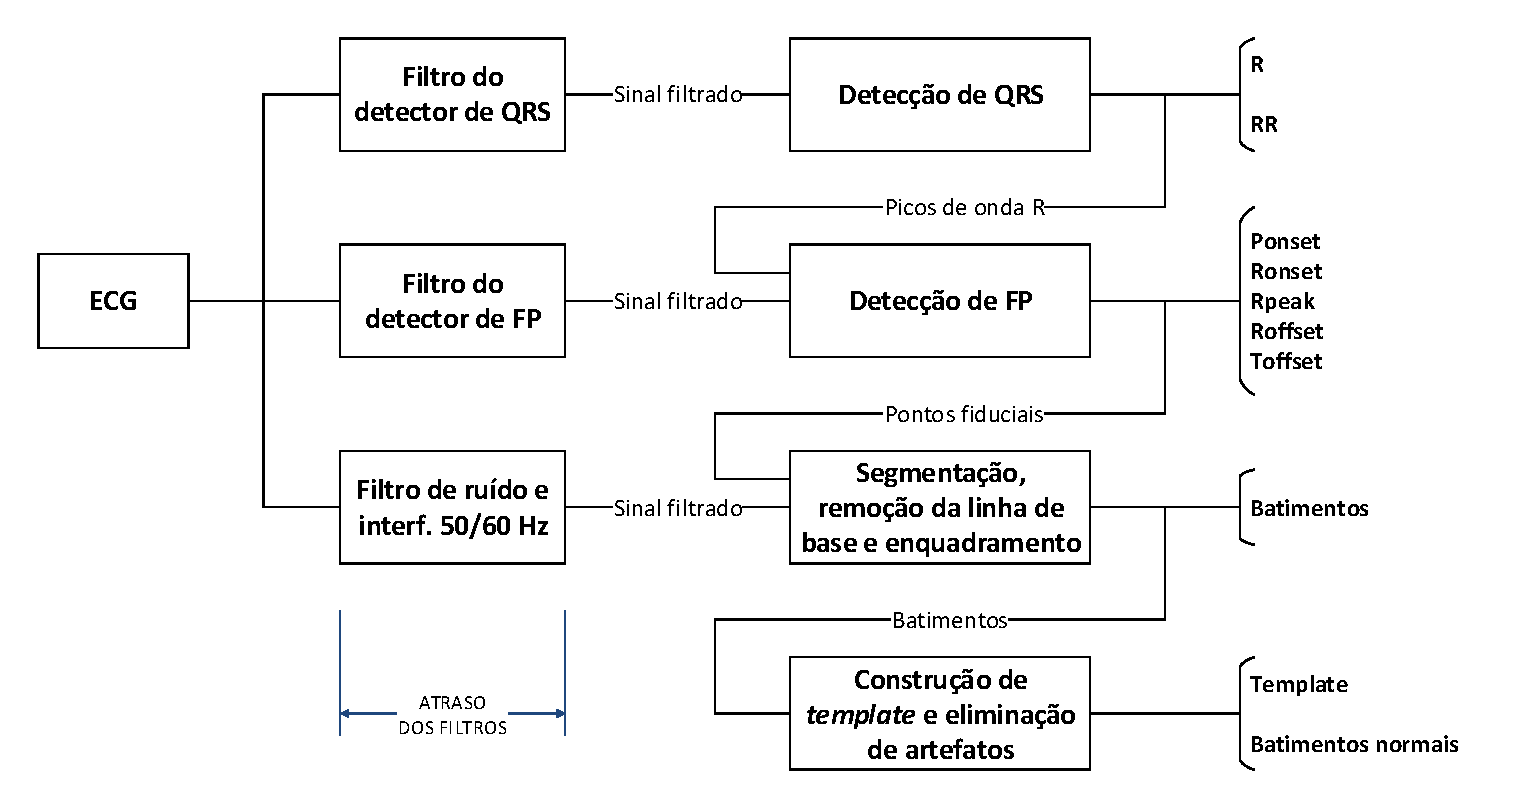
\includegraphics[width=450pt]{figures/chap6-preprocessing-diagram.pdf}
    \caption[Diagrama de blocos da estratégia de pré-processamento]{Diagrama de blocos da estratégia de pré-processamento. Produzida no Microsoft Visio.}
    \label{fig:preprocessdiag}
\end{figure}

O primeiro item de informação provém da detecção de QRS. O algoritmo utilizado para tal fim é aquele descrito por Pan e Tompkins \cite{Pan1985}. Este algoritmo é também descrito no livro de um dos autores \cite[pp. 245-262]{Tompkins1993} e avaliado em outro artigo \cite{Hamilton1986}. A escolha deste algoritmo segue a escolha feita por dois dos métodos de detecção de isquemia, o de Mohebbi e Moghadam e o de Gopalakrishnan et al., mas também se deve ao fato de que ele constitui uma técnica robusta e tradicional na área de processamento de sinais biomédicos.

Na prática, a lista R é desnecessária aos métodos de detecção de isquemia, pois, como veremos mais adiante, os batimentos são segmentados e embutidos num quadro (\emph{frame}) de tamanho pré-definido. Sendo este tamanho um número ímpar e estabelecendo que os batimentos dentro do quadro estejam centralizados no pico de onda R, tem-se que o pico está sempre no ponto central do quadro, dispensando o uso da lista na etapa de extração.

Esta lista serve, porém, para apuração do resultado dos métodos, em termos das métricas introduzidas no capítulo \ref{chap:chapter4}. Sabemos que as anotações do ECG fornecem a localização dos batimentos conforme auditada por especialistas e, portanto, se faz necessário para fins de avaliação conhecer a localização obtida pelo detector de QRS. Dadas duas listas de pontos, há um algoritmo que faz o casamento cruzado entre elas. Isto é, que combina batimentos de uma lista com os da outra contanto que estejam muito próximos temporalmente. Este algoritmo é apresentado na rotina \texttt{match\_qrs} (código-fonte \ref{lst:matchqrs}), escrita em código MATLAB.

O segundo item de informação não é simplesmente a diferença entre picos de onda R sucessivos, mas sim uma estimativa média do intervalo RR calculada a cada novo batimento. A estimativa tem portanto o efeito de ``suavizar'' a medida, eliminando variações demasiado abrutas de frequência cardíaca\footnote{a frequência cardíaca (em batimentos por minuto) pode ser obtida a partir do intervalo RR, pela expressão $\frac{60f_s}{RR}$, onde $f_s$ é a frequência de amostragem do conversor A/D}. A lista RR provém do mesmo algoritmo de detecção de QRS, sendo necessária por dois motivos: primeiro porque o método de Rocha et al. emprega uma técnica de determinação do ponto J (definido logo adiante) fazendo uso da medida de frequência cardíaca; segundo porque Gopalakrishnan et al. lançam mão do intervalo RR na sua etapa de extração.

O terceiro item advém de um algoritmo proposto por Yan Sun et al. \cite{Sun2005}. Originalmente, o procedimento faz a marcação dos seguintes pontos de interesse (ou \emph{fiducial points}):
\begin{description}
    \item[$\{P_{onset}, P_{peak}, P_{offset}\}$] pontos inicial, de pico e final da onda P;
    \item[$\{Q_{onset}, Q_{peak}, Q_{offset}\}$] pontos inicial, de pico e final da onda Q;
    \item[$\{R_{onset}, R_{peak}, R_{offset}\}$] pontos inicial, de pico e final da onda R;
    \item[$\{S_{onset}, S_{peak}, S_{offset}\}$] pontos inicial, de pico e final da onda S; e
    \item[$\{T_{onset}, T_{peak}, T_{offset}\}$] pontos inicial, de pico e final da onda T.
\end{description}
Contudo, apenas os pontos de início da onda P, os pontos da onda R e o ponto final da onda T são realmente necessários para os fins deste trabalho. $R_{onset}$ e $R_{offset}$ servem para realizar a busca de dois outros pontos de interesse: o isoelétrico e o $J$, definidos informalmente abaixo.
\begin{mydef}
    Ponto isoelétrico é o local designado para o batimento onde este apresenta amplitude de ``nível zero'' antes do início da onda R. Isto é, o ponto à esquerda de $R_{onset}$ que pode ser considerado como referência para a troca de polaridade das amplitudes do batimento cardíaco.
\end{mydef}
\begin{mydef}
    Ponto $J$ é o local designado para o batimento onde o seu ``traço'' se torna mais horizontal do que vertical, após o término da onda R. Isto é, o ponto à direita de $R_{offset}$ que pode ser considerado como início de um período de inatividade elétrica do coração.
\end{mydef}

O ponto isoelétrico (aqui, apelidado de $I$) e o ponto $J$ são obtidos por um algoritmo distinto, descrito por Daskalov em \cite{Daskalov1998}. A técnica em essência detecta as bordas do batimento cardíaco com auxílio da derivada de primeira ordem do sinal. Quem a sugere é Mohebbi e Moghadam, para uso na delimitação do segmento ST. Os mesmos pontos são necessários ao método de Rocha et al., por dois motivos: primeiro porque o ponto $I$ servirá de referência para a estimativa do desvio ST, medido como a diferença entre as amplitudes no ponto $J$ e naquele; segundo porque o ponto $J$ serve como separador dos segmentos utilizados na etapa de extração do método (rever seção \ref{sec:rocha}). Rocha et al., que sugerem o uso do algoritmo de Sun citado anteriormente, requerem os pontos inicial e final do batimento, $P_{onset}$ e $T_{offset}$, principalmente por dois motivos: para remoção da linha de base e para delimitação dos segmentos usados na etapa de extração. A identificação da linha de base é feita por uma aproximação polinomial envolvendo as bordas de cada batimento, daí a necessidade destes pontos.

No método de Mohebbi e Moghadam, a remoção da linha de base seria alcançada através de interpolação \emph{spline} cúbica, segundo um artigo de Badilini \cite{Badilini1991}. A técnica requer conhecimento apenas da localização dos picos de onda R e é de fácil implementação para o caso de trincas -- isto é, usando, além do batimento atual, o seu precedente e o sucessor. Contudo, num sistema de tempo-real, haverá necessidade de aguardar a detecção de um novo batimento cardíaco para que possa ser feita a interpolação para o batimento atual, o que incorre em um atraso equivalente a um batimento. No pior caso, o batimento seguinte pode nunca ser detectado. Ademais, a interpolação é mais precisa se se lançar mão das derivadas do sinal nas extremidades, implicando a necessidade de dois pontos adicionais (um antes do precedente e um depois do sucessor). Finalmente, a aproximação se deteriora à medida que a frequência cardíaca diminui, pois então o maior afastamento entre os pontos na interpolação prejudica o ajuste de amplitudes em torno do ponto central. Em virtude dessas desvantagens, neste trabalho foi escolhida a técnica anterior.

O quarto item de informação é constituído pelos próprios batimentos cardíacos, depois de segmentados, filtrados, sem linha de base e enquadrados num \emph{frame} de tamanho fixo. O tamanho do \emph{frame} foi estabelecido como $1,2$ vezes o número de amostras em $1$ segundo do sinal. De acordo com \cite{Clifford2006}, a duração de um ciclo cardíaco está entre 0,6 e 1 segundo. Dando uma margem de tolerância de $0,2$ segundos ao valor máximo, garante-se que a vasta maioria dos batimentos caibam no \emph{frame}. Caso o tamanho resultante seja um número par, o incrementa-se de 1 para que a condição previamente especificada seja satisfeita (pico de onda R no centro do emph{frame}).

A segmentação, portanto, consiste em delimitar o batimento cardíaco por seus pontos inicial e final, centralizá-lo pelo seu pico de onda R e enquadrá-lo no \emph{frame}. O enquadramento remove qualquer trecho que esteja fora do quadro, tanto à esquerda quanto à direita do centro, bem como preenche com zeros caso ``sobre'' espaço no quadro. A remoção da linha de base ocorre antes deste procedimento, porque utiliza a informação completa do sinal do batimento. Conforme sugerido por Rocha et al., a técnica para identificação da linha de base é adaptada de Wolf \cite{Wolf2004}, que faz a interpolação usando um polinômio de primeiro grau.

O quarto item corresponde ao \emph{template}, que é construído progressivamente ao longo da execução. O uso de \emph{template} se faz necessário para o método de Mohebbi e Moghadam, que o utiliza para extrair um modelo de segmento ST. Os autores também o requerem afim de eliminar artefatos que foram identificados erroneamente como batimento pelo detector QRS. A eliminação se dá por meio de uma medida de erro, neste caso a distância Euclideana, obtida pela norma da diferença entre os vetores que descrevem o template e o batimento avaliado. Aproveitando-se dessa exigência, incorporou-se um algoritmo iterativo de construção do \emph{template} à etapa de pré-processamento. Dessa forma, todos os métodos de detecção de isquemia se beneficiam da eliminação de artefatos, o que propicia uma comparação mais justa. Para o método de Mohebbi e Moghadam, que necessita de um \emph{template} explicitamente, toma-se então a versão de \emph{template} que ocorre depois de processados os primeiros 30 ciclos cardíacos.

A filtragem do sinal de ECG para remoção de ruído e interferência, conforme ilustra a figura \ref{fig:preprocessdiag}, é realizada em paralelo com a detecção de QRS e de FP. Essa filtragem se dá pela aplicação de dois filtros IIR: um passa-baixas de Butterworth seguindo a especificação dada por Rocha et al., para redução de ruído de alta-frequência; e um rejeita-faixas Chebyshev tipo I com banda de rejeição de 2 Hz, para eliminação da interferência da rede elétrica. O projeto desses filtros, diferentemente do projeto dos filtros da detecção QRS e FP, é feito de antemão por intermédio do MATLAB, para várias frequências de amostragem comuns em eletrocardiografia.

Uma decisão de projeto que merece menção é o fato de ter-se aberto mão da transformada discreta de Wigner-Ville. Este procedimento era requerido pelo método de Rocha et al. para a localização dos pontos $I$ e $J$. Entretanto, a implementação desta transformada em linguagem de programação tradicional não é trivial. Ela envolve o uso de variáveis complexas, da transformada de Fourier discreta (DFT) e da transformada de Hilbert, além de ser bastante custosa em termos de processamento. O uso de variáveis complexas significa que deve-se trabalhar com dois vetores em memória, um para a parte real e outro para a parte imaginária do sinal. O uso da transformada de Fourier implica que devemos selecionar e incorporar um algoritmo de FFT (\emph{Fast Fourier Transform}) ao ferramental do trabalho. A transformada de Hilbert, que, segundo os autores, é necessária para obtenção de um sinal analítico antes da aplicação da Wigner-Ville, parece ser tão cheia de peculiaridades que alguns professores a consideram matéria de pós-graduação. Esses fatores tornam a implementação mais complicada e demorada, não só pela complexidade mas porque todo código desenvolvido deve ser testado e validado. 

Há ainda o fato de que, dado um vetor de tamanho $n$, são necessários $n$ cálculos de DFT para obter a transformada de Wigner-Ville do vetor. Não bastasse isso, a matriz resultante deve passar por operações de valor absoluto e de soma, em que as linhas correspondentes a baixas frequências são superpostas para formar o vetor subjacente à busca dos pontos desejados. As duas últimas observações indicam que o procedimento exige bastante processamento. E de fato isso ocorre: fez-se uma tentativa de implementação usando a linguagem MATLAB (que possui funções prontas de DFT, Hilbert, manipulação de matrizes e de números complexos), e determinou-se que o tempo de processamento deste item perfazia mais da metade do tempo de extração de características do método.

Outra questão é que, nesta tentativa de implementação da transformada de Wigner-Ville, o resultado da identificação dos pontos $I$ e $J$ foi medíocre. O que ocorre é que os pontos de mínimo não são tão bem definidos e, muitas vezes, não existem dentro dos intervalos de busca (lembre-se de que os próprios autores não deixam claro os limites dos intervalos). Em virtude de todas estas considerações, decidiu-se não utilizar a transformada de Wigner-Ville para localização dos pontos $I$ e $J$. Em vez disso, reaproveitou-se a técnica utilizada por Mohebbi e Moghadam (aquela que faz uso de diferenciação e \emph{thresholding}).

\subsection*{Implementação}

A implementação aconteceu de três formas, cada uma em um momento diferente. Primeiro criou-se um ambiente de trabalho usando a ferramenta computacional MATLAB. Neste caso, diversas rotinas de tratamento dos sinais de ECG foram implementadas em código MATLAB, e serviram para testar e validar o funcionamento da estratégia adotada. Em seguida, criou-se códigos na linguagem C que realizam as mesmas tarefas de maneira equivalente, e estes foram validados pela comparação de seus resultados com aqueles obtidos usando o código MATLAB. Num terceiro momento, construiu-se um modelo de simulação em tempo real, usando a ferramenta Simulink do MATLAB. Nesta implementação, utilizou-se a linguagem C++, que oferece recursos de orientação a objetos e permite uma melhor organização do código-fonte.

O desenvolvimento em C e em C++ se deu através do próprio MATLAB, que oferece uma API (\emph{Application Programming Interface}) para uso e compilação de códigos C/C++ na sua plataforma. Não serão feitas aqui referências ao código em C nem C++, apenas ao código MATLAB. Além disso, devido ao tamanho do trabalho, somente algumas rotinas em MATLAB serão apresentadas, todas no apêndice \ref{app:matlab} desta monografia. Caso o leitor deseje visualizar o código completo, tanto em MATLAB quanto em C ou C++, refira-se ao seguinte link: \url{https://github.com/dsogari/tg-ecp-ufrgs}. Ali estará o repositório do trabalho desenvolvido disponível para \emph{download} gratuito. Este repositório será atualizado constantemente até a conclusão do trabalho, o que pode não coincidir com a entrega desta monografia.

Os sinais de ECG são os da base de dados ST-T da Sociedade Européia de Cardiologia \cite{Taddei1992}, obtidos a partir do \emph{website} PhysioBank.org da PhysioNet \cite{Goldberger2000}. A leitura dos arquivos da base foi realizada com auxílio do pacote de software WFDB, disponibilizado gratuitamente pelo mesmo \emph{site}. Na verdade, para facilitar o trabalho no MATLAB, criou-se algumas rotinas que encapsulam as chamadas do WFDB e produzem arquivos .mat contendo todas as informações de um ECG. Assim, para ler um arquivo de ECG basta carregar o .mat correspondente usando as funções nativas do MATLAB, que são bastante simples e eficientes.

Uma estrutura em MATLAB contém as amostras do sinal e outras informações a respeito deste, como a frequência de amostragem, o valor de referência e a resolução do conversor A/D, anotações, entre outras. Esta estrutura serve como entrada para a etapa de pré-processamento. A etapa começa pela filtragem do sinal de ECG, descrita em detalhes a seguir.

A filtragem para detecção de complexos QRS se dá pela função \texttt{qrs\_filter} (código \ref{lst:qrsfilter}). Esta função recebe como parâmetros as amplitudes do sinal de ECG e a frequência de amostragem, $f_s$. Ela retorna o sinal filtrado e o atraso total dos filtros, $d_{QRS}$. Os filtros deste procedimento são quatro: um passa-baixas de segunda ordem\footnote{\label{fnt:note1}esta ordem não diz respeito ao número de coeficientes do filtro, mas sim tem a ver com os coneitos apresentados no capítulo \ref{chap:chapter3}, no que tange à técnica de projeto de filtros FIR com coeficientes inteiros} com frequência de corte em aproximadamente 11 Hz; um passa-altas de primeira ordem\footnote{Ver nota de rodapé \ref{fnt:note1}}. com frequência de corte em aproximadamente 5 Hz; um diferenciador de 5 pontos; e um filtro de média-movel com largura aproximada de 150 ms. A figura \ref{fig:qrsfilter} mostra o diagrama de blocos da filtragem QRS, enquanto as figuras \ref{fig:qrssignals1} e \ref{fig:qrssignals2} ilustram os diversos sinais intermediários dessa filtragem.

\begin{figure}[ht]
    \centering
    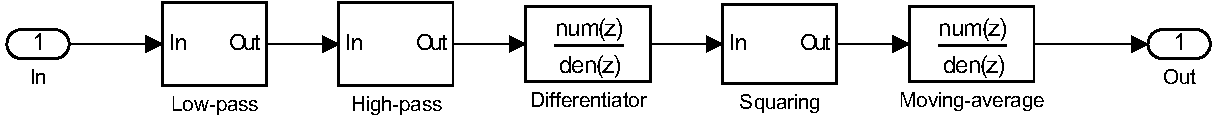
\includegraphics[width=450pt]{figures/chap6-qrs-filter.pdf}
    \caption[Diagrama de blocos do filtro QRS]{Diagrama de blocos do filtro para detecção de complexos QRS.}
    \label{fig:qrsfilter}
\end{figure}

\begin{figure}[ht]
    \centering
    \begin{subfigure}[b]{.3\textwidth}
        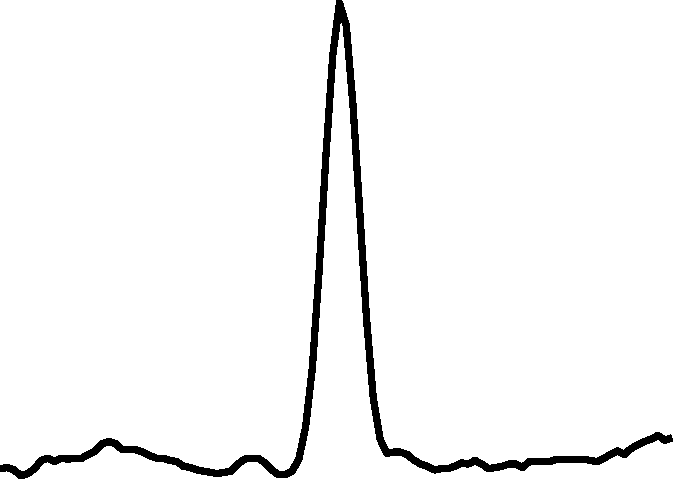
\includegraphics[width=\textwidth]{figures/chap6-original.pdf}
        \caption{Sinal de ECG}
    \end{subfigure}
    \begin{subfigure}[b]{.3\textwidth}
        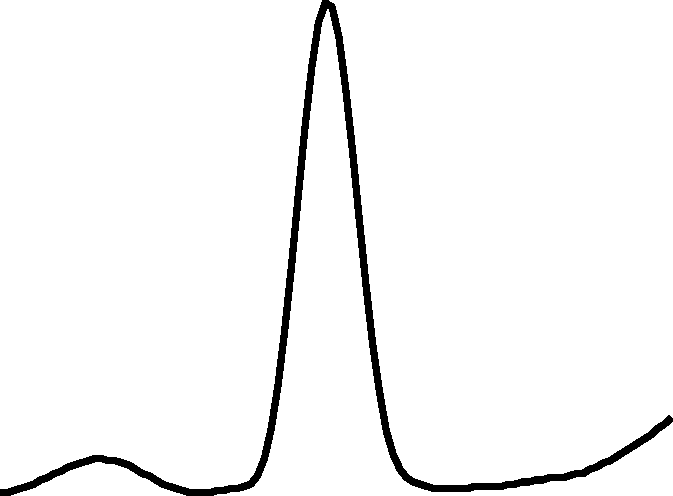
\includegraphics[width=\textwidth]{figures/chap6-lowpass.pdf}
        \caption{Saída do passa-baixas}
    \end{subfigure}
    \begin{subfigure}[b]{.3\textwidth}
        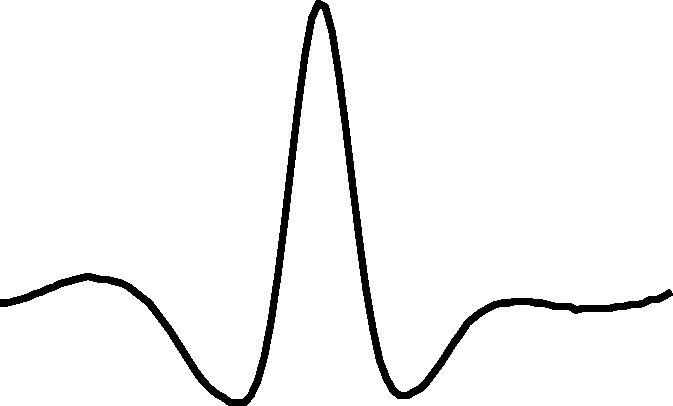
\includegraphics[width=\textwidth]{figures/chap6-highpass.pdf}
        \caption{Saída do passa-altas}
    \end{subfigure}
    \caption[Sinais intermediários da filtragem QRS]{Sinais intermediários da filtragem QRS.}
    \label{fig:qrssignals1}
\end{figure}

\begin{figure}[ht]
    \centering
    \begin{subfigure}[b]{.3\textwidth}
        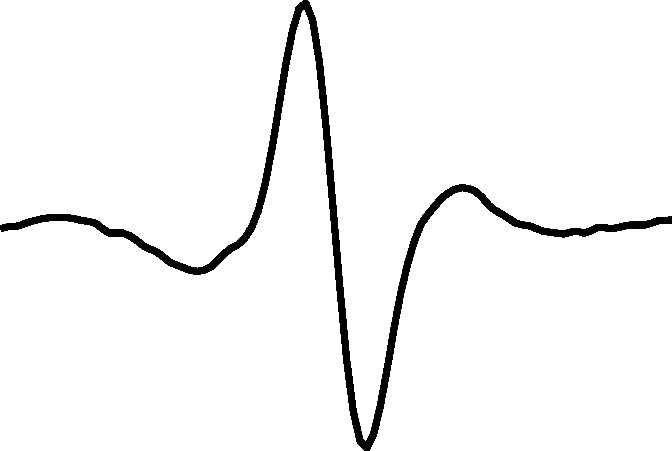
\includegraphics[width=\textwidth]{figures/chap6-differentiator.pdf}
        \caption{Saída do diferenciador}
    \end{subfigure}
    \begin{subfigure}[b]{.3\textwidth}
        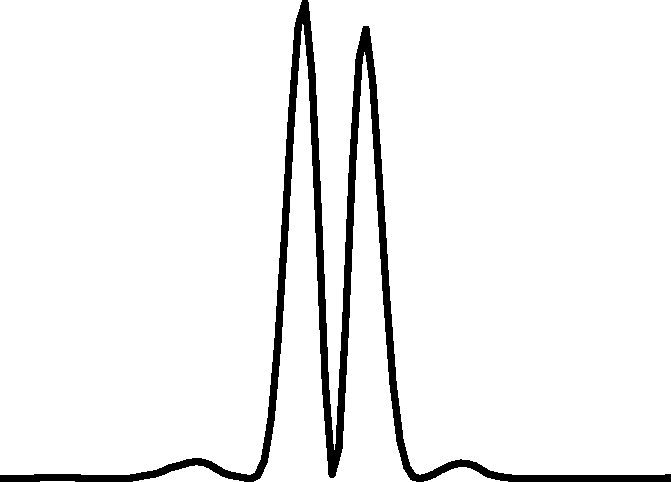
\includegraphics[width=\textwidth]{figures/chap6-squaring.pdf}
        \caption{Saída do operador quadrado}
    \end{subfigure}
    \begin{subfigure}[b]{.3\textwidth}
        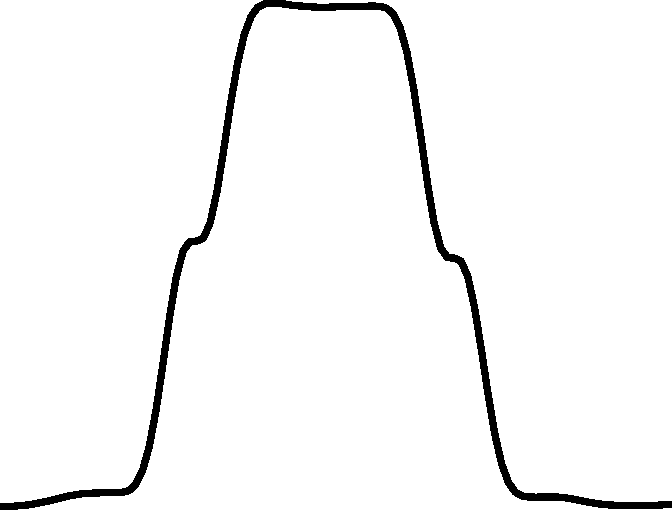
\includegraphics[width=\textwidth]{figures/chap6-moving-average.pdf}
        \caption{Saída do média-móvel}
    \end{subfigure}
    \caption[Sinais intermediários da filtragem QRS (continuação)]{Sinais intermediários da filtragem QRS (continuação).}
    \label{fig:qrssignals2}
\end{figure}

A filtragem para detecção de pontos de interesse se dé pela função \texttt{fp\_filter} (código \ref{lst:fpfilter}). Esta função recebe como parâmetros as amplitudes do sinal de ECG, a frequência de amostragem e o atraso $d_{QRS}$. Ela retorna dois sinais, um que corresponde à derivada de primeira ordem do sinal de entrada suavizado e outro que é a derivada morfológica \cite{Sun2002} do sinal suavizado. Os filtros deste procedimento são quatro: um passa-baixas de segunda ordem\footnote{Ver nota de rodapé \ref{fnt:note1}} com frequência de corte em aproximadamente 11 Hz; um filtro de média-móvel com largura de aproximadamente 50 ms; um diferenciador de dois pontos; e um filtro de média-movel com largura aproximada 150 ms.

A filtragem para remoção de ruído se dé pela função \texttt{noise\_filter} (código \ref{lst:noisefilter}). Esta função recebe como parâmetros as amplitudes do sinal de ECG, a frequência de amostragem, a frequência da rede elétrica, $f_m$, e novamente o atraso $d_{QRS}$. Ela retorna o sinal filtrado, isto é, sem ruído de alta frequência e sem interferência da rede elétrica. Há dois filtros neste procedimento: um passa-baixas de Butterworth de quarta ordem com frequência de corte em aproximadamente 40 Hz; e um rejeita-faixas de quarta ordem Chebyshev tipo I, com frequência central em $f_m$ e largura da banda de rejeição de aproximadamente 2 Hz.

Os atrasos das três filtragens seriam dados a grosso modo por: $d_{QRS} \approx 0.18f_s$, $d_{FP} \approx 0.09f_s$ e $d_{noise} \approx 0.01f_s$. Entretanto, deseja-se ``emparelhar'' os sinais filtrados. Isto é, fazer com que eles estejam na mesma linha de tempo após a filtragem. Isso facilita o trabalho dos detectores na etapa de pré-processamento. Sabendo que $d_{QRS}$ é o maior dos três atrasos, tem-se que as demais devem ser igualadas àquela. A equivalência de atrasos é alcançada pela introdução de filtros passa-tudo, com um atraso dado pela diferença entre $d_{QRS}$ e $d_{FP}$ ou entre $d_{QRS}$ e $d_{noise}$. Para uma frequência de amostragem de 250 Hz, que é aquela da base de dados utilizada, tem-se $d_{QRS} = 46.5$ amostras. Também vale dizer que a frequência da rede elétrica usada nos testes foi 50 Hz, uma vez que a base de dados é européia.

O próximo passo é detectar os batimentos. A função que realiza tal procedimento é \texttt{detect\_qrs} (código \ref{lst:detectqrs}). Ela recebe como parâmetros as amplitudes do sinal filtrado pelos filtros QRS e a taxa de amostragem. Ela retorna a localização aproximada dos picos de onda R e uma estimativa média dos intervalos RR. Existem cinco componentes principais no laço deste algoritmo: detecção de picos, atualização de \emph{thresholds}, determinação de complexos QRS, atualização de medidas de intervalo RR e busca de QRS em retrospecto (\emph{searchback}). Para cada pico detectado, verifica-se se a amplitude é maior que um \emph{threshold}. Se for, então o pico é candidato a ser de um complexo QRS. Medidas de nível de ruído e de sinal são atualizadas de acordo com a decisão tomada para o pico. O \emph{threshold} é computado em função desses níveis. Caso nenhum complexo QRS seja detectado dentro de um determinado período, a busca em retrospecto é ativada para recuperar um possível complexo perdido. A localização do pico do complexo, que quase sempre corresponde ao pico de onda R, não é identificada exatamente pelo algoritmo. O importante é saber que há um complexo QRS nos instantes próximos ao pico detectado no sinal filtrado. A localização exata no ECG é obtida pela detecção de pontos fiduciais, descrita a seguir.

A detecção de pontos fiduciais se dá pela função \texttt{detect\_fp} (código \ref{lst:detectfp}). Ela recebe como parâmetros os dois sinais filtrados pela filtragem FP e a lista R fornecida pelo detector QRS. Sua saída é uma lista com os pontos fiduciais correspondentes a cada item da lista R. A busca é dividida em três partes. Em primeiro lugar são detectados os pontos referentes à onda R ($R_{peak}$, $R_{onset}$ e $R_{offset}$). Em segundo lugar, tendo $R_{onset}$, detecta-se o pico e o início da onda P ($P_{peak}$ e $P_{onset}$). Lembre-se de que $P_{peak}$ não será necessário posteriormente, mas é imprescindível para a busca de $P_{onset}$. Por último, tendo $R_{offset}$, detecta-se o pico e o fim da onda T ($T_{peak}$ e $T_{offset}$). Novamente, $T_{peak}$ não será necessário para a etapa de extração, mas serve para encontrar $T_{offset}$. A busca é feita com ajuda de algumas rotinas especiais: \texttt{search\_peak\_abs}, \texttt{search\_first\_mark} e \texttt{search\_best\_mark}. Em particular, a busca dos picos ($R_{peak}$, $P_{peak}$ e $T_{peak}$) desconsidera a polaridade do sinal. Isto é, um pico negativo é identificado da mesma maneira que um pico positivo, utilizando a rotina \texttt{search\_peak\_abs}. As figuras \ref{fig:fpsignalN} e \ref{fig:fpsignalM} ilustram os sinais de ECG e o da derivada morfológica, com a localização dos pontos fiduciais.

\begin{figure}[p]
    \centering
    \begin{subfigure}[b]{.6\textwidth}
        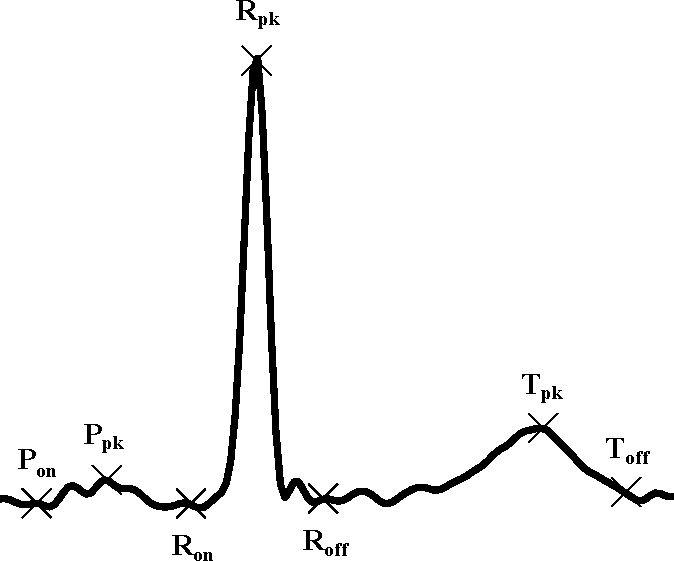
\includegraphics[width=\textwidth]{figures/chap6-fiducial-points1.pdf}
        \caption{Sinal de ECG}
        \label{fig:fpsignalN}
    \end{subfigure}
    \vskip20pt
    \begin{subfigure}[b]{.6\textwidth}
        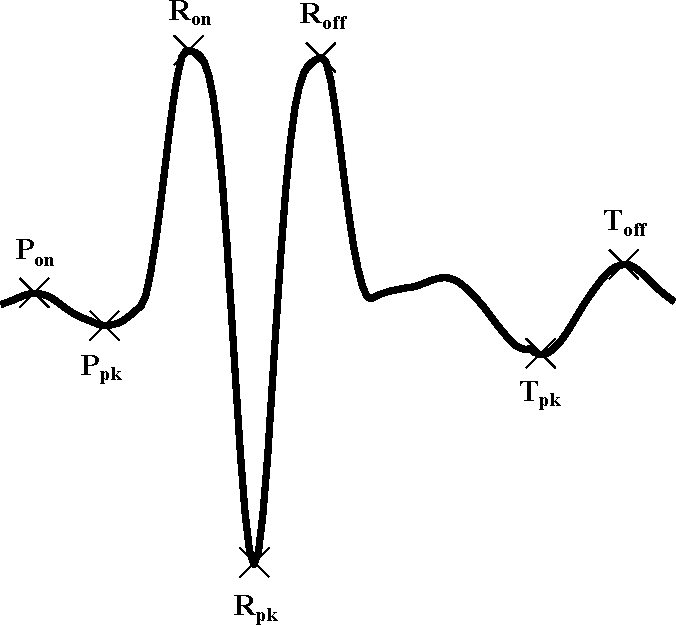
\includegraphics[width=\textwidth]{figures/chap6-fiducial-points3.pdf}
        \caption{Sinal da derivada morfológica}
        \label{fig:fpsignalM}
    \end{subfigure}
    \caption[Sinais da filtragem FP e respectivos pontos]{Sinais da filtragem FP e respectivos pontos.}
\end{figure}

A segmentação dos batimentos pode agora ser realizada, pois tem-se as marcações $P_{onset}$ e $T_{offset}$. Também com base nestes pontos, pode-se encontrar um polinômio de primeiro grau que melhor se ajusta à reta que conecta ambos. Mais especificamente, toma-se uma média das amplitudes nos cinco pontos próximos a $P_{onset}$ e nos cinco pontos próximos a $T_{offset}$. Com as médias, calcula-se os parâmetros da reta que os liga. Em cada ponto do batimento, subtrai-se da amplitude original o valor da reta avaliado naquele ponto. Tem-se assim um batimento cuja linha de base é o próprio eixo horizontal de nível zero (ou isoelétrico). A figura \ref{fig:baseline} ilustra o procedimento de remoção (ou normalização) da linha de base.

\begin{figure}[ht]
    \centering
    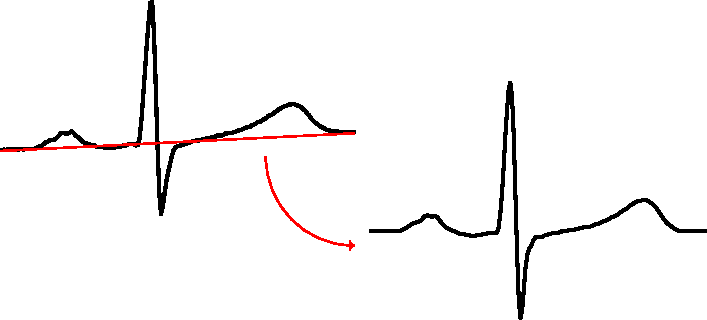
\includegraphics[width=400pt]{figures/chap6-baseline-removal.pdf}
    \caption[Procedimento de remoção da linha de base]{Procedimento de remoção da linha de base.}
    \label{fig:baseline}
\end{figure}

Após a remoção da linha de base, o batimento é enquadrado num \emph{frame}, da maneira como foi explicada no início desta seção. A função que realiza estes procedimentos é \texttt{extract\_beats} (código \ref{lst:extractbeats}), com suas rotinas auxiliares \texttt{polyfit\_baseline} e \texttt{frame\_beat}. Os parâmetros de entrada de \texttt{extract\_beats} são as amplitudes do sinal filtrado pelos filtros de ruído, a lista FP e a taxa de amostragem. Sua saída é composta pela lista de batimentos extraídos e uma nova lista FP cujos valores dizem respeito à localização dos pontos de interesse no \emph{frame} (e não mais no ECG).

Finalmente, toma lugar a construção de \emph{template} e a remoção de artefatos. Para tanto, é usada a função \texttt{build\_template} (código \ref{lst:buildtemplate}). Esta função recebe como parâmetro a lista de batimentos e uma constante que diz a taxa de adaptação do \emph{template}. Por exemplo, uma taxa de $R$ significa que as amplitudes do \emph{template} obedecem à regra $T_i[n] = T_{i-1}[n] + R^{-1}\left(B_i[n] - T_{i-1}[n]\right), 0 \leq n \leq N-1$, com $N$ igual ao tamanho do \emph{frame} dos batimentos. Esta é a equação de recorrência de um filtro de média-móvel exponencial com constante de decaimento igual a $1/R$. No entanto, o \emph{template} só é atualizado se a diferença, $E$, entre o \emph{template} e o batimento atual for menor que um \emph{threshold}, $C$. Este \emph{threshold} é calculado pela mesma relação recursiva: $C_i = C_{i-1} + R^{-1}\left(E_i - C_{i-1}\right)$.

O erro $E_i$ é a medida de diferença na i-ésima iteração, dada pela distância Euclideana: $E_i = \|B_i - T_i\|$. Na verdade, dois valores de \emph{threshold} são mantidos, um que equivale a 3 vezes o valor do erro médio e o outro, a 4 vezes o mesmo valor. Assim, se o erro na iteração atual for menor que o primeiro \emph{threshold}, então o batimento é considerado muito bom e tanto o \emph{template} quanto o \emph{threshold} são atualizados. Senão, se o erro estiver acima do segundo \emph{threshold}, então o batimento é considerado como artefato e descartado. Se o erro cair no intervalo entre os dois \emph{thresholds}, o batimento é considerado bom e mantido sem que haja alteração de \emph{template} ou de \emph{threshold}. A figura \ref{fig:artifact} ilustra a comparação feita para determinar se um batimento é um artefato ou não.

\begin{figure}[ht]
    \centering
    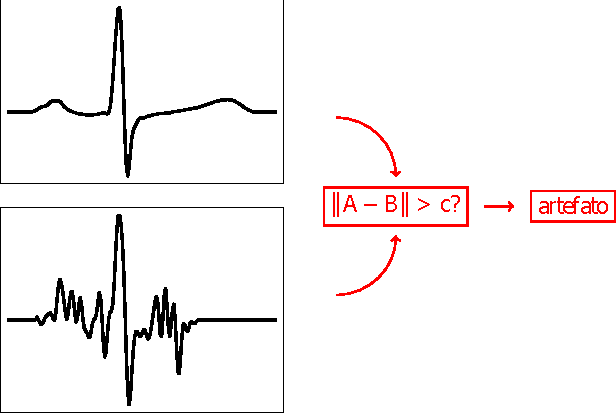
\includegraphics[width=400pt]{figures/chap6-artifact-removal.pdf}
    \caption[Procedimento de remoção de artefatos]{Procedimento de remoção de artefatos.}
    \label{fig:artifact}
\end{figure}

\section{Projeto da extração de características}

\subsection*{Método de Rocha et al.}
A extração de características do método de Rocha começa pela identificação do ponto $J$ através da técnica de Pang \cite{Pang2005}. A função que realiza este procedimento é \texttt{pang\_jpoint}. Ela recebe como parâmetro os intervalos RR e retorna a localização do ponto $J$ de acordo com o intervalo em que se encontra a frequência cardíaca, conforme mostra a tabela \ref{tab:pangpoints}.

\begin{table}[ht!]
    \centering
    \begin{tabular}{cc}
    \toprule
    Frequência cardíaca (em BPM) & Ponto de medida\\
    \midrule
    $<100$        & $R+120$ ms\\
    $100-110$  & $R+112$ ms\\
    $110-120$  & $R+104$ ms\\
    $>120$       & $R+100$ ms\\
    \bottomrule
\end{tabular}
    \caption[Localização do ponto $J$ determinada com base na frequência cardíaca]{Localização do ponto $J$ determinada com base na frequência cardíaca.}
    \label{tab:pangpoints}
\end{table}

Em seguida, o algoritmo de bordas é empregado para a busca do ponto isoelétrico e também para uma nova estimativa do ponto $J$. A função \texttt{edge\_detection} (código \ref{lst:edgedetection}), que recebe como parâmetros o sinal do batimento, pontos de início e fim, além de um \emph{threshold}, faz a busca do ponto desejado no intervalo, retornando este como saída. A busca do ponto $I$ se dá pela aplicação da função no intervalo à esquerda de $R_{peak}$, enquanto a busca de $J$ se dá no intervalo à direita de $R_{peak}$.

Com estes pontos, obtêm-se uma medida do desvio de segmento ST, dado pela diferença entre as amplitudes do batimento nos pontos $J$ e aquela avaliada no ponto $I$. Essas duas medidas são as primeiras a compor o conjunto de características do método de Rocha et al. A figura \ref{fig:rochastdev} ilustra o procedimento de obtenção do desvio ST.

\begin{figure}[ht]
    \centering
    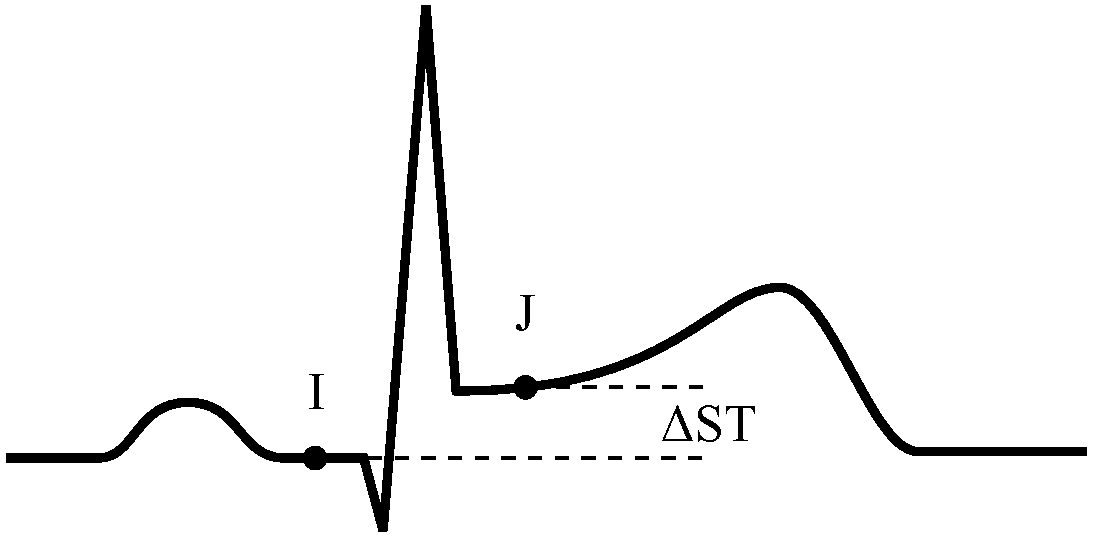
\includegraphics[width=350pt]{figures/chap6-rocha-stdev.pdf}
    \caption[Cálculo do desvio de segmento ST]{Cálculo do desvio de segmento ST no método de Rocha et al.}
    \label{fig:rochastdev}
\end{figure}

O próximo passo é seccionar o batimento em dois segmentos: um contendo o complexo QRS e outro contendo a onda T. O primeiro segmento vai do ponto $I$ até o ponto $J$, enquanto o segundo vai deste até o ponto final do batimento ($T_{offset}$). Cada um destes segmentos é então reamostrado para um sinal de 64 amostras. A função do MATLAB para reamostragem é \texttt{resample}. Ela recebe como parâmetros o sinal que se deseja reamostrar, um fator de interpolação $p$ e um fator de dizimação $q$, retornando um sinal de largura $\lceil\frac{p}{q}\rceil$ vezes a largura original. Internamente, essa função faz o projeto de um filtro passa-baixas FIR, necessário ao algoritmo de reamostragem.

Na implementação em C da reamostragem, foi usada a técnica de projeto de filtros por truncagem da resposta ideal, conforme vista no capítulo \ref{chap:chapter3}. O filtro projetado possui as seguintes especificações: largura da região de transição de 2 Hz, frequência de corte em $\frac{\pi}{\max\left(p,q\right)}$ radianos e uso da janela Hamming (que apresenta atenuação média de 41 dB na banda de rejeição). Note que o projeto é refeito a cada nova chamada de reamostragem, pois a especificação depende do tamanho do sinal original. A figura \ref{fig:rochaseg} mostra a delimitação dos segmentos no batimento.

\begin{figure}[ht]
    \centering
    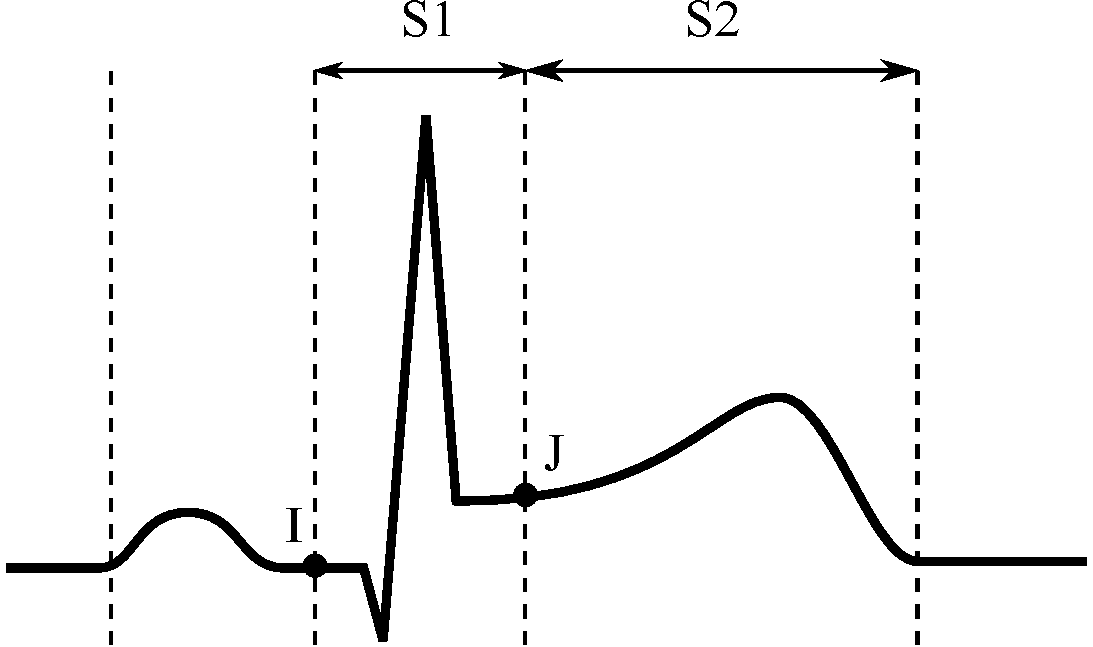
\includegraphics[width=350pt]{figures/chap6-rocha-segments.pdf}
    \caption[Particionamento do batimento em dois segmentos]{Particionamento do batimento em dois segmentos para o método de Rocha et al.}
    \label{fig:rochaseg}
\end{figure}

Os segmentos devidamente reamostrados servem como operando no produto matricial que fornece os coeficientes da expansão em funções de Hermite, sendo o outro operando a matriz discutida no capítulo \ref{chap:chapter5} para o método de Rocha et al. Há uma matriz para o primeiro segmento e outra para o segundo segmento, cada qual com seu fator de dilatação (5 e 8, para ser exato). Ambas possuem 6 linhas e 64 colunas, de modo que o produto com o vetor coluna contendo as 64 amostras do segmento correspondente resulta nos coeficientes desejados. A figura \ref{fig:rochaherm} ilustra o procedimento de expansão em funções de Hermite e extração dos coeficientes.

\begin{figure}[ht]
    \centering
    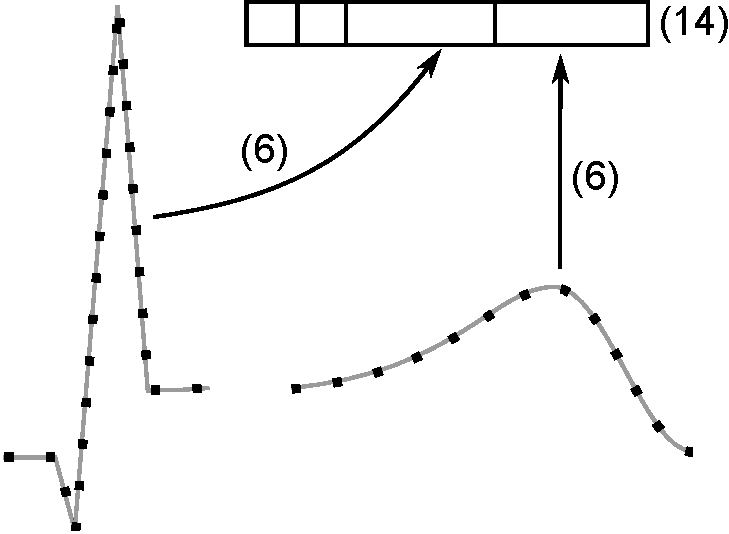
\includegraphics[width=300pt]{figures/chap6-rocha-hermite.pdf}
    \caption[Aproximação dos segmentos por funções de Hermite]{Aproximação dos segmentos por funções de Hermite para o método de Rocha et al.}
    \label{fig:rochaherm}
\end{figure}

Portanto, ao final da extração do método de Rocha et al., obtêm-se um conjunto de 14 características, quais sejam: duas medidas de desvio de segmento ST; seis coeficientes da expansão de Hermite do primeiro segmento; e seis coeficientes da expansão do segundo segmento. A função responsável pelo garimpo de todos estes itens é \texttt{rocha\_features} (código \ref{lst:rochafeatures}), auxiliada pelas rotinas \texttt{pang\_jpoints}, \texttt{rocha\_ijpoints}, \texttt{rocha\_stdev}, \texttt{rocha\_segments} e \texttt{rocha\_hermite} (códigos \ref{lst:pangjpoints}, \ref{lst:rochaijpoints}, \ref{lst:rochastdev}, \ref{lst:rochasegments} e \ref{lst:rochahermite} respectivamente).

\subsection*{Método de Mohebbi e Moghadam}
A etapa de extraçao do método de Mohebbi e Moghadam começa com a localização do ponto $J$, pelo mesmo procedimento já mencionado, o da função \texttt{edge\_detection}. Depois, extrai-se o segmento ST, que inicia no ponto $J$ e se estende por 160 ms (ou 40 amostras, numa frequência de amostragem de 250 Hz). O segmento é reamostrado pra 20 amostras e sua diferença com o segmento ST do \emph{template} é obtida por uma simples operação de subtração. A figura \ref{fig:mohebbistseg} ilustra como é feita a extração do segmento ST, enquanto a figura \ref{fig:mohebbistdiff} mostra como é feita a composição do vetor de características do método.

\begin{figure}[ht]
    \centering
    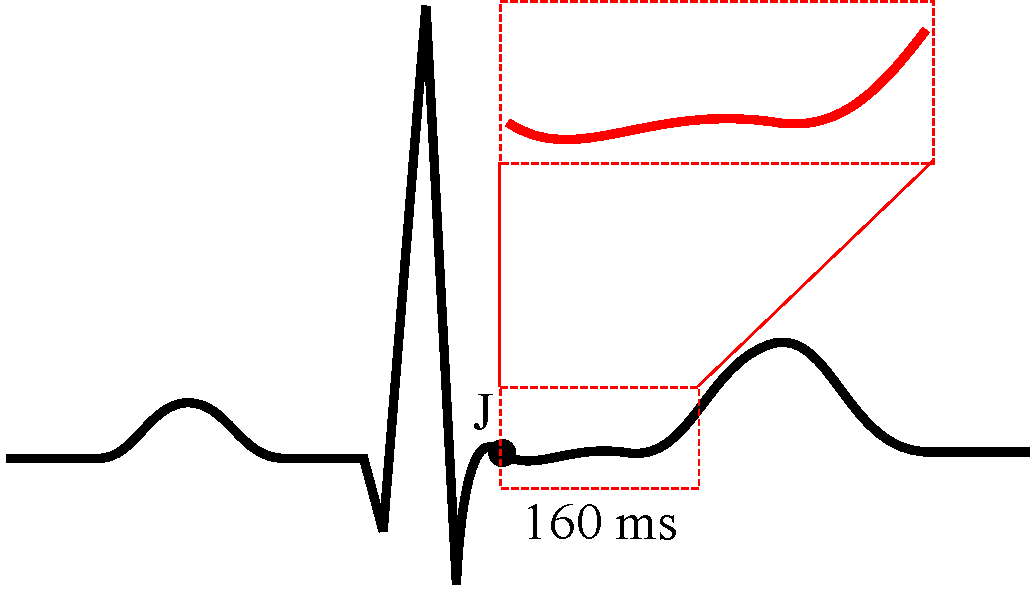
\includegraphics[width=350pt]{figures/chap6-mohebbi-stseg.pdf}
    \caption[Obtenção do segmento ST a partir do ponto $J$]{Obtenção do segmento ST a partir do ponto $J$ no método de Mohebbi e Moghadam.}
    \label{fig:mohebbistseg}
\end{figure}

\begin{figure}[ht]
    \centering
    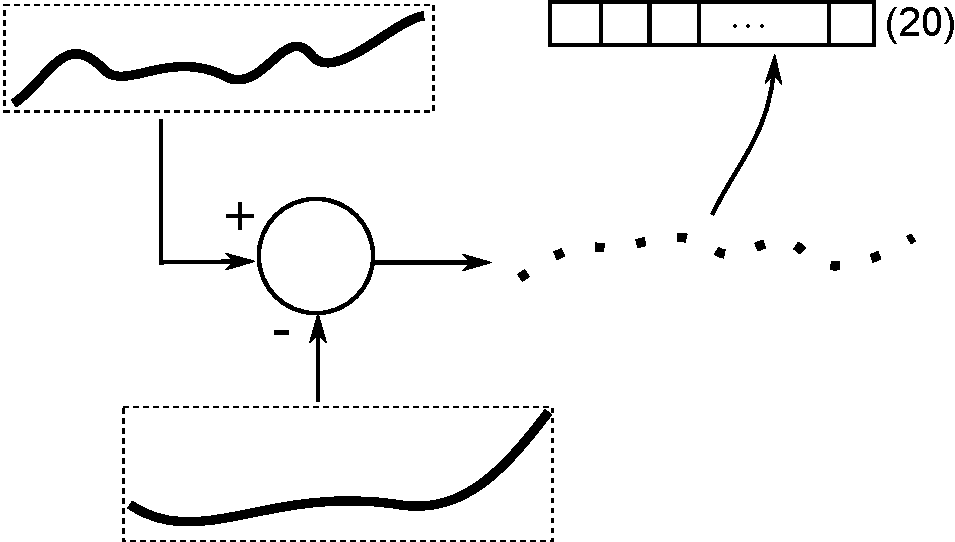
\includegraphics[width=350pt]{figures/chap6-mohebbi-stdiff.pdf}
    \caption[Diferença entre o segmento ST de teste e o de referência]{Diferença entre o segmento ST de teste e o de referência, para composição das características do método de Mohebbi e Moghadam.}
    \label{fig:mohebbistdiff}
\end{figure}

Note-se que o ponto $J$ e o segmento ST do \emph{template} são extraídos apenas uma vez, tão logo o \emph{template} se faça presente. A versao de \emph{template} utilizda é aquela computada após o 30\ordm batimento. A função que executa estes procedimentos é \texttt{mohebbi\_features} (código \ref{lst:mohebbifeatures}), suportada pelas rotinas auxiliares \texttt{mohebb\_ijpoints}, \texttt{mohebb\_isegments} e \texttt{mohebb\_istdiff} (códigos \ref{lst:mohebbijpoints}, \ref{lst:mohebbisegments} e \ref{lst:mohebbistdiff}, respectivamente).

\subsection*{Método de Gopalakrishnan et al.}
A extração do método de Gopalakrishnan et al. é bastante simples. Primeiro, um segmento é extraído contendo todo o batimento. Ele está centralizado no pico de onda R (ou o centro do \emph{frame}) e possui largura igual ao intervalo RR correspondente ao batimento em questão. Subsequentemente, a função de reamostragem é aplicada para produzir um sinal de tamanho fixo igual a 250 amostras. A figura \ref{fig:gopalakseg} mostra como é feita a delimitação do batimento, enquanto a figura 

\begin{figure}[ht]
    \centering
    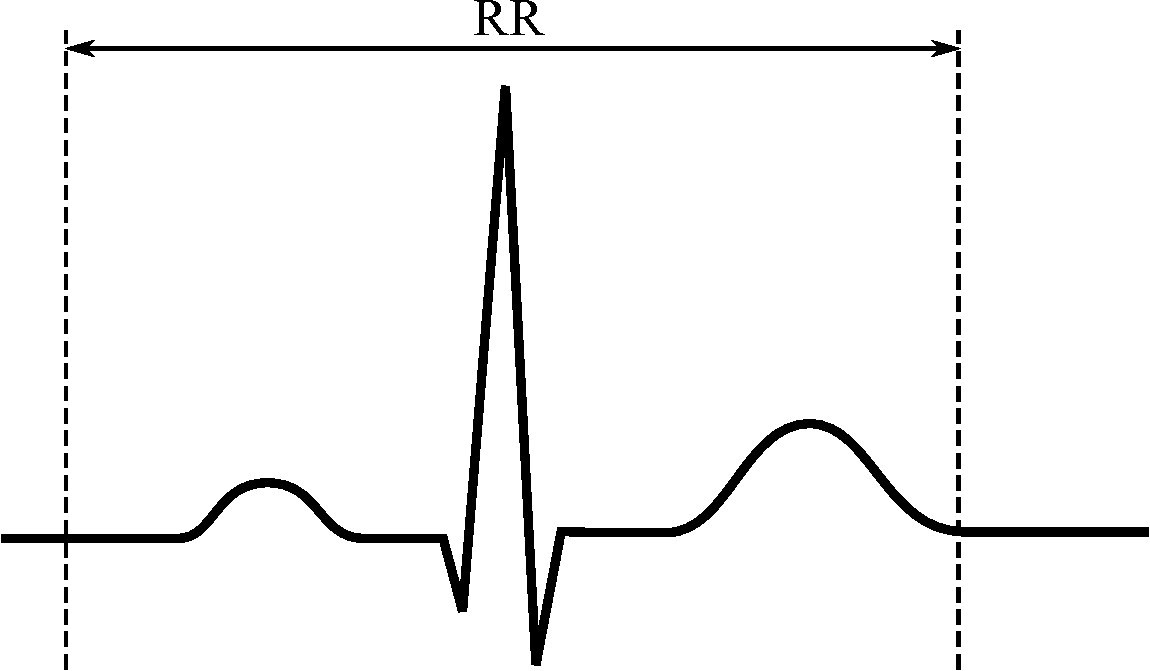
\includegraphics[width=300pt]{figures/chap6-gopalak-segment.pdf}
    \caption[Delimitação do batimento e centralização no intervalo RR]{Delimitação do batimento e centralização no intervalo RR, para uso o método de Gopalakrishnan et al.}
    \label{fig:gopalakseg}
\end{figure}

Finalmente, ocorre o produto matricial entre a matriz de funções discretas de Hermite (ver capítulo \ref{chap:chapter3}), com 50 linhas e 250 colunas, e o vetor coluna com as 250 amostras do batimento. O resultado é um conjunto de 50 coeficientes, que compõem o conjunto de caracteristicas do método. A função que realiza estes procedimentos é \texttt{gopalak\_features} (código \ref{lst:gopalakfeatures}), juntamente com as rotinas auxiliares \texttt{gopalak\_segments} e \texttt{gopalak\_hermite} (códigos \ref{lst:gopalaksegments} e \ref{lst:gopalakhermite}, respectivamente). A figura \ref{fig:gopalakherm} ilustra o procedimetno de aproximação do batimento em funções de Hermite discretas e extração dos respectivos coeficientes.

\begin{figure}[ht]
    \centering
    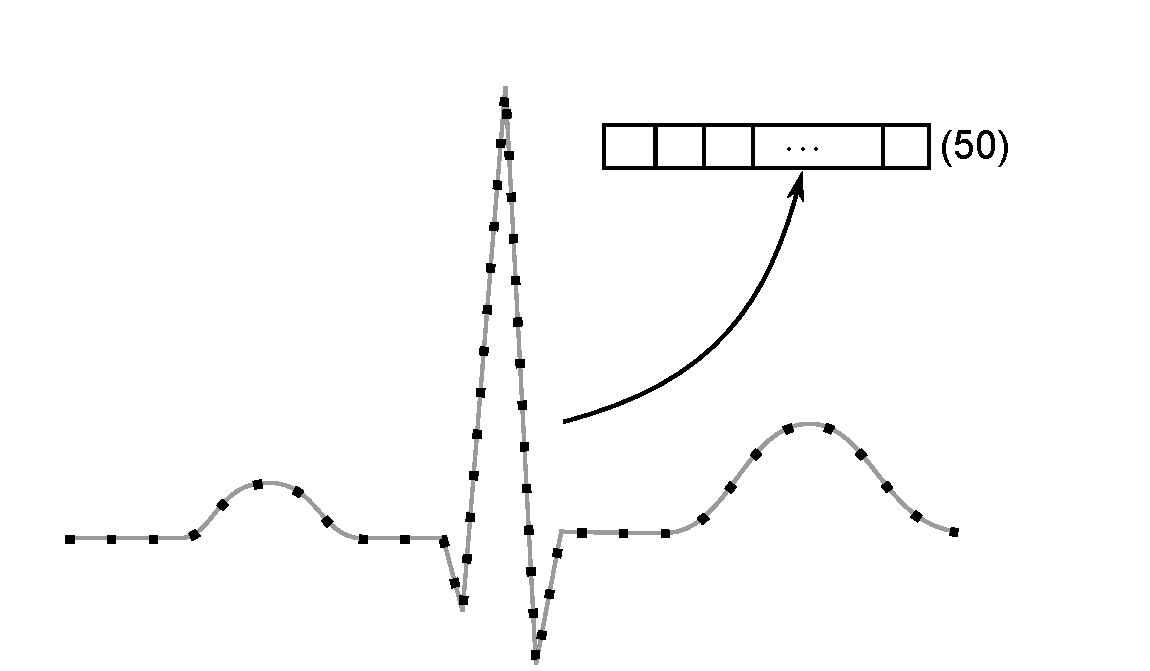
\includegraphics[width=400pt]{figures/chap6-gopalak-hermite.pdf}
    \caption[Aproximação do batimento por funções discretas de Hermite]{Aproximação do batimento por funções discretas de Hermite e composição do vetor de características do método de Gopalakrishnan et al.}
    \label{fig:gopalakherm}
\end{figure}

\section{Projeto da classificação}

Para a etapa de classificação, cada autor sugere uma estrutura diferente de redes neurais, bem como procedimentos distintos de treinamento das mesmas. As tabelas \ref{tab:nnspecs} e \ref{tab:trainspecs} mostram os diversos aspectos dos três esquemas de classificação propostos.

\begin{table}[ht!]
    \centering
    \begin{tabular}{p{4cm}p{3.8cm}p{3.8cm}p{3.8cm}}
    \toprule
    \backslashbox{Item}{Método} & Rocha et al. & Mohebbi e Moghadam & Gopalakrishnan et al.\\ 
    \midrule
    Função de transferência   & tangente sigmóide & log-sigmóide & tangente sigmóide\\
    Função de normalização    & não especificado & não especificado & não especificado\\
    N\ordm de entradas        & 14 & 20 & 50\\
    N\ordm de saídas          & 1 & 1 & 2\\
    Intervalo da saída        & [-1,1] & [0,1] & [-1,1]\\
    N\ordm de camadas ocultas & 2 & 1 & 1\\
    N\ordm de neurônios       & depende da derivação & 20 & não especificado\\
    N\ordm de redes           & 2 & 1 & 5\\
    \bottomrule
\end{tabular}
    \caption[Especificações da estrutura das redes neurais segundo cada autor]{Especificações da estrutura das redes neurais segundo cada autor.}
    \label{tab:nnspecs}
\end{table}

\begin{table}[ht!]
    \centering
    \begin{tabular}{p{4cm}p{3.8cm}p{3.8cm}p{3.8cm}}
    \toprule
    \backslashbox{Item}{Método} & Rocha et al. & Mohebbi e Moghadam & Gopalakrishnan et al.\\ 
    \midrule
    Função de treinamento     & Levenberg-Marquardt (\texttt{trainlm}) & \emph{Backpropagation} adaptativo (\texttt{traingdx}) & Gradiente conjugado (\texttt{trainscg})\\
    Característica utilizada  & ST & ST & ST e T\\
    Proporção de ocorrência   & não especificado & 0.169 & não especificado\\
    Registros utilizados      & conferir tabela \ref{tab:selection} & conferir tabela \ref{tab:selection} & não especificado\\
    Divisão do conjunto para \emph{cross-validation} & não especificado & não especificado & não especificado\\
    N\ordm de amostras & depende da derivação & 18047 & 236\\
    Considera derivações separadamente & sim & não & não\\
    \bottomrule
\end{tabular}
    \caption[Especificações do esquema de treinamento segundo cada autor]{Especificações do esquema de treinamento segundo cada autor.}
    \label{tab:trainspecs}
\end{table}

\begin{table}[ht!]
    \centering
    \begin{tabular}{lp{5cm}p{6cm}}
    \toprule
    \backslashbox{Derivação}{Método} & Rocha et al. (descartados) & Mohebbi e Moghadam (utilizados)\\ 
    \midrule
    D3    & -- & --\\
    MLI   & e0207 & --\\
    MLIII & e0109, e0121, e0609, e0613 & e0103, e0105, e0113, e0119, e0147\\
    V1    & e0403 & --\\
    V2    & e0415 e0603 & --\\
    V3    & -- & --\\
    V4    & e0119 e0161 & e0103, e0105, e0113, e0119, e0147\\
    V5    & e0207, e0213, e0303, e0405 & --\\
    \bottomrule
\end{tabular}
    \caption[Seleção de registros da base pelos métodos]{Seleção de registros da base pelos métodos.}
    \label{tab:selection}
\end{table}

Assim como na etapa de pré-processamento, isso gera um problema prático: a implementação fica difícil e propensa a erros, pois a quantidade de código a ser escrito, mantido e testado é maior. Há novamente aqui uma motivação para criar um código único, que sirva para todos os métodos. Não apenas essa abordagem tende a tornar mais justa a comparação entre os métodos, mas facilita a implementação e encurta o tempo de desenvolvimento, do qual se carece. A solução então é combinar as diversas escolhas dos autores e encontrar uma combinação boa e conveniente para o esquema de classificação final. A seguir são descritas as escolhas feitas e o porquê de cada uma.

\begin{itemize}
    \item Algoritmo de treinamento \texttt{trainlm}: é o padrão do MATLAB; usado pelo método de Rocha et al.; é geralmente o mais rápido a convergir, segundo a documentação do MATLAB.
    \item Função de transferência tangente sigmóide (\texttt{tansig}): usado por dois dos métodos.
    \item Função de normalização \texttt{mapstd} (média 0 e desvio padrão 1): segundo colegas de trabalho, é a mais comumente utilizada.
    \item Divisão aleatória dos dados na proporção 75/15/15: como nenhum dos autores explicita a sua escolha para fins de \emph{cross-validation}, será utilizada a divisão padrão do MATLAB, que é de 75\% para treinamento, 15\% para validação e 15\% para teste (de modo aleatório).
    \item Saída única: o treinamento é mais rápido do que com 2 ou mais saídas (verificado experimentalmente); quando as saídas dizem respeito a informações independentes (caso do terceiro método), as chances de sucesso são maiores usando duas redes separadas.
    \item 2 camadas ocultas com número aleatório de neurônios: intuitivamente, 2 camadas devem fornecer resultado melhor do que uma; um número fixo de neurônios durante o treinamento seria interessante apenas se se comprovasse que um número é melhor que outro.
    \item Saída indica presença ou ausência da característica: tanto a característica de desvio de segmento ST quanto a da onda T na verdade são decompostas em outras 2, que são a elevação ou depressão do segmento ST e a elevação ou depressão da onda T. As possíveis classes então seriam aquelas dadas na tabela \ref{tab:nnclasses}. No entanto, considerando as redes com saída única, tem-se um número elevado de redes a serem treinadas. Portanto, decidiu-se utilizar a presença ou ausência de cada característica separadamente, mas sem distinguir entre elevação ou depressão. O resultado são duas redes: uma indicando presença/ausência de desnivelamento ST e a outra, presença/ausência de desnivelamento da onda T.
    \item Uso das proporções de ocorrência da base: apenas um dos autores sugere a composição do conjunto de dados usando uma proporção específica de batimentos normais \emph{versus} isquêmicos. Assim, decidiu-se levantar estatísticas sobre a proporção de ocorrência de cada característica na base, e estas servirão como referência na seleção dos dados. Mais detalhes serão discutidos na seção \ref{sec:tests}.
    \item Uma rede para cada derivação: na implementação das etapas de processamento anteriores, percebeu-se que as formas de onda -- e, consequentemente, as características extraídas -- de diferentes derivações são bastante díspares; Rocha et al. também apontam este fato e dizem ser a separação uma boa escolha para melhorar os resultados. Como a base possui ECGs de 8 derivações diferentes, tem-se um total de 8 redes para cada método.
    \item Seleção dos dados de acordo com resultados de ECGs individuais: num primeiro momento, os conjuntos de dados continham exatamente os mesmos registros de ECG sugeridos por cada autor (ver tabela \ref{tab:selection}). Contudo, os resultados obtidos foram pífios. Ao fazer o treinamento das redes para cada registro individualmente, notou-se que muitos dos resultados eram bons, enquanto outros estavam aquém do esperado. Concluiu-se que os vetores de características da fase de extração para estes últimos não representavam corretamente os batimentos detectados. Porquanto não há uma maneira simples e automatizada de avaliar a consistência dos dados extraídos, optou-se por utilizar os próprios resultados individuais como critério de seleção. Mais detalhes serão discutidos na seção \ref{sec:tests}.
\end{itemize}

\begin{table}[ht!]
    \centering
    \begin{tabular}{lccc}
    \toprule
    \backslashbox{ST}{T} & Normal & Elevado & Deprimido\\
    \midrule
    Normal    & $C_{11}$ & $C_{12}$ & $C_{13}$ \\
    Elevado   & $C_{21}$ & $C_{22}$ & $C_{23}$ \\
    Deprimido & $C_{31}$ & $C_{32}$ & $C_{33}$ \\
    \bottomrule
\end{tabular}
    \caption[Possíveis classes do procedimento de classificação]{Possíveis classes do procedimento de classificação.}
    \label{tab:nnclasses}
\end{table}

Há que se mencionar que os dois primeiros métodos não utilizam as características de desvio da onda T no seu procedimento de classificação. Rocha et al. deixam claro esta escolha, enquanto Mohebbi e Moghadam não explicitam a sua. Acredita-se que estes tenham utilizado apenas o desvio de segmento ST, pois é com base neste segmento que o vetor de características do método é extraído. Gopalakrishnan et al., por outro lado, dizem claramente que utilizam as duas características (ST e T). Assim, tem-se um total de (2 métodos $\times$ 1 característica $+$ 1 método $\times$ 2 características) $\times$ 8 derivações $=$ 32 redes neurais a serem treinadas para uma dada seleção de conjuntos de dados.

A classe a que pertence um batimento é dada pela condição $y>0$, onde $y$ é um valor real entre -1 e 1, correspondente à saída de uma rede neural. A condição satisfeita indica que a característica observada está presente, e o contrário é verdadeiro ($y\leq 0 \rightarrow$ característica ausente). Para julgar se um batimento é isquêmico, basta perguntar se $y>0$ nos dois primeiros métodos, ou perguntar se $y_1>0$ || $y_2>0$ no método de Gopalakrishnan et al., pois este tem duas redes (ST e T).

Outra questão importante é manter a proporção de ocorrência das características na população quando se faz uma seleção dos dados de treinamento das redes neurais. Este é o conceito de \textbf{estratificação}. Se existir muito mais batimentos com a característica observada do que realmente existe na população, a probabilidade de que a rede produza muitos falsos positivos é grande. Portanto, deve-se procurar manter a proporção original da população (que seria a base de ECGs).

Alguns códigos da etapa de classificação em MATLAB são apresentados no apêndice \ref{app:matlabclass}. As rotinas principais de treinamento são \texttt{train\_network} e \texttt{train\_networks} (códigos \ref{lst:trainnetwork} e \ref{lst:trainnetworks}); as rotinas \texttt{generate\_datasets} e \texttt{generate\_lead\_dataset} (códigos \ref{lst:generatedatasets} e \ref{lst:generateleaddataset}) são relativas à seleção de dados para composição dos conjuntos de treinamento, a ser discutida na próxima seção. A figura \ref{fig:vectorsandnets} dá uma ideia geral de como fica etapa de classificação.

\begin{figure}[ht]
    \centering
    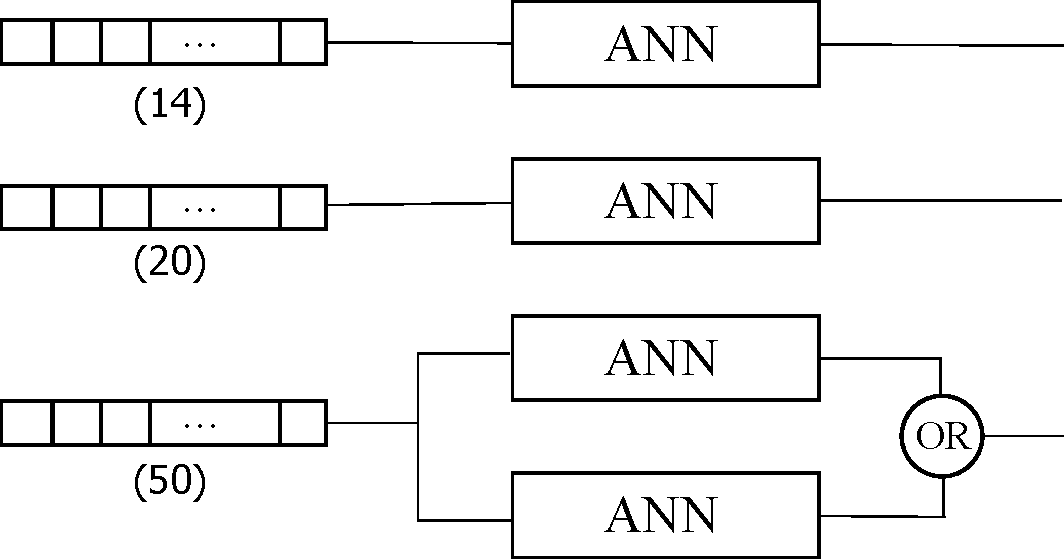
\includegraphics[width=350pt]{figures/chap6-vectors-and-networks.pdf}
    \caption[Visualização da etapa de classificação dos métodos]{Visualização da etapa de classificação dos métodos.}
    \label{fig:vectorsandnets}
\end{figure}


\section{Projeto dos testes}
\label{sec:tests}

Conforme discutido anteriormente, fez-se necessário o levantamento das proporções de ocorrência das características de isquemia (ST e T) na base de ECGs. Já foi mencionado que a base contém registros de 8 derivações diferentes. Cada uma destas apresenta o seu percentual de ocorrência tanto no quesito ST como no T. A título de exemplo, as figuras \ref{fig:mlistclass} e \ref{fig:v4stclass} mostram num gráfico do tipo ``pizza'' os percentuais encontrados para a característica ST nas derivações MLI e V4, respectivamente. Da mesma forma, as figuras \ref{fig:mlitclass} e \ref{fig:v4tclass} ilustram a distribuição de ocorrência da característica T. O mesmo estudo foi feito para as demais derivações, de modo a possuir todos os percentuais de ocorrência necessários à construção dos conjuntos de dados.

\begin{figure}[ht]
    \centering
    \begin{subfigure}[b]{.4\textwidth}
        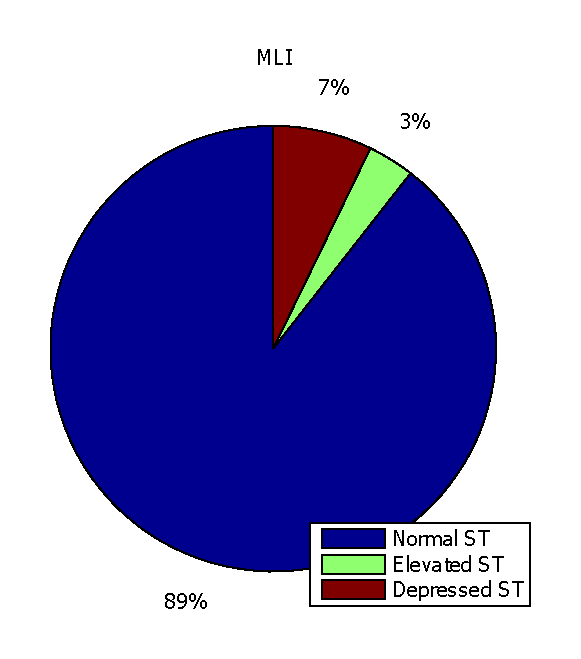
\includegraphics[width=\textwidth]{figures/chap6-mli-st-class-dist.pdf}
        \caption{Derivação MLI}
        \label{fig:mlistclass}
    \end{subfigure}
    \begin{subfigure}[b]{.4\textwidth}
        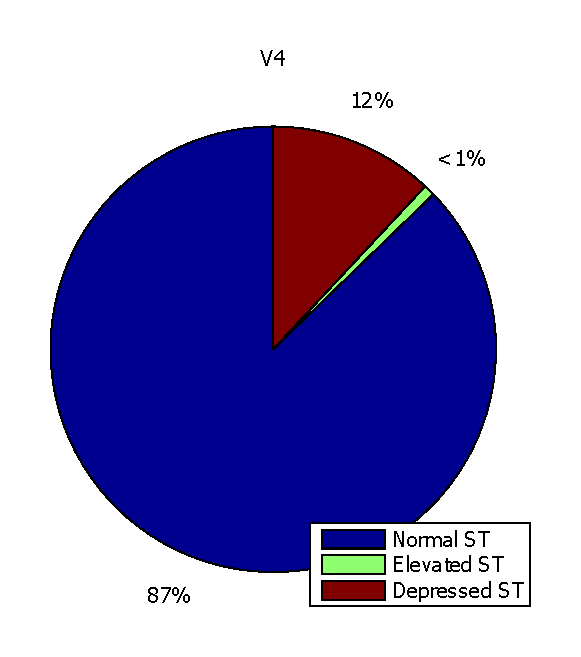
\includegraphics[width=\textwidth]{figures/chap6-v4-st-class-dist.pdf}
        \caption{Derivação V4}
        \label{fig:v4stclass}
    \end{subfigure}
    \caption[Gráficos de distribuição da característica ST na base]{Gráficos de distribuição da característica ST na base. Produzidos no MATLAB.}
\end{figure}

\begin{figure}[ht]
    \centering
    \begin{subfigure}[b]{.4\textwidth}
        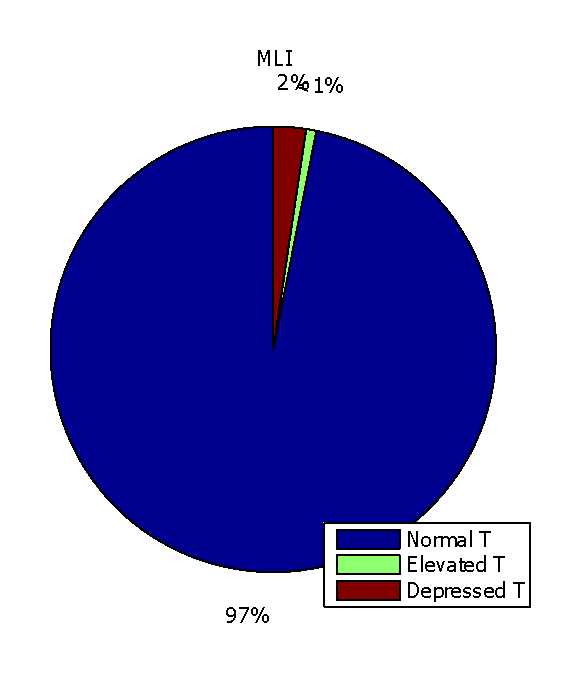
\includegraphics[width=\textwidth]{figures/chap6-mli-t-class-dist.pdf}
        \caption{Derivação MLI}
        \label{fig:mlitclass}
    \end{subfigure}
    \begin{subfigure}[b]{.4\textwidth}
        \includegraphics[width=\textwidth]{figures/chap6-v4-t-class-dist.pdf}
        \caption{Derivação V4}
        \label{fig:v4tclass}
    \end{subfigure}
    \caption[Gráficos de distribuição da característica T na base]{Gráficos de distribuição da característica T na base. Produzidos no MATLAB.}
\end{figure}

Foi discutido também que a proposta original dos autores para seleção dos dados não rendeu resultados satisfatórios. Portanto, far-se-á um estudo para determinar quais os registros de ECG da base que mais prejudicam o desempenho geral. Quer-se então criar 5 configurações diferentes de seleção de conjuntos de dados para treinamento:

\begin{description}
    \item[Configuração 1] proposta original dos autores, mantendo inclusive o número de batimentos.
    \item[Configuração 2] proposta criada com base no desempenho obtido com redes individuais.
    \item[Configuração 3] da configuração anterior, faz-se uma junção (ou \emph{merger}) entre as listas dos diferentes métodos, privilegiando a decisão da maioria.
    \item[Configuração 4] mesma seleção da configuração 3, só que restringindo o número de batimentos selecionados (mas mantendo a estratificação).
    \item[Configuração 5] conjunto completo extraído da base, sem descarte
\end{description}

Nas configurações 1 e 2, cada método possui sua própria seleção de registros e número de batimentos, enquanto nas demais a seleção se mantém igual para os três métodos. Um resumo desta estratégia pode ser visualizado na figura \ref{fig:selection}. Na figura, os canais 0 ou 1 dizem respeito a um dos vetores de amostras de ECG contidos num registro da base (todos contêm 2 canais).

\begin{figure}[ht]
    \centering
    \includegraphics[width=470pt]{figures/chap6-selection-scheme.pdf}
    \caption[Esquema de seleção de conjuntos de dados]{Esquema de seleção de conjuntos de dados para o treinamento das redes neurais. Produzido no Microsoft Visio.}
    \label{fig:selection}
\end{figure}

Com esta estratégia, haverá 5 configurações $\times$ 32 $=$ 160 redes neurais a serem treinadas. Também seria necessário apresentar, no capítulo seguinte, 8 tabelas de resultados individuais e 20 tabelas de resultados coletivos, pois são 5 configurações $\times$ 4 instâncias de treinamento e teste (Rocha et al. para ST, Mohebbi e Moghadam para ST e Gopalakrishnan et al. para ST e T). A fim de não poluir o espaço do próximo capítulo com diversas tabelas, será feita uma análise um pouco diferente: primeiro será apresentada uma tabela de exemplo contendo a primeira instância de teste; em seguida serão mostradas tabelas contendo o resultado médio de todos os registros para o caso individual e de todas as derivações para o caso coletivo. Dessa forma, haverá cerca de 9 ou 10 tabelas concisas, contendo as informações relevantes para uma análise comparativa de confiabilidade dos métodos.

\section{Resumo}

Neste capítulo foram apresentados os projetos das etapas de pré-processamento, extração e classificação, bem como um projeto dos testes a serem realizados para comparação de desempenho dos métodos.

Primeiramente, na etapa de pré-processamento, viu-se que há a quatro procedimentos principais: a detecção de complexos QRS; a detecção de pontos de interesse; a segmentação e eliminação da linha de base; e por último a construção de \emph{template} e eliminação de artefatos. Os três primeiros são precedidos, cada qual, por uma filtragem do sinal de ECG. A filtragem realça características que são importantes ao procedimento correspondente. O resultado desta etapa são os batimentos cardíacos, os intervalos RR, os pontos de interesse em cada batimento e também um \emph{template} de batimento normal. Vale lembrar que os procedimentos desta etapa são os mesmos para todos os métodos de detecção de isquemia.

Na etapa de extração, os batimentos submetem-se às técnicas de processamento propostas pelos autores dos métodos, embora com algumas modificações. No método de Rocha et al., o desvio de segmento ST é calculado com base nos pontos $I$ e $J$, e os coeficientes de Hermite são obtidos após uma nova segmentação do batimento em duas partes, com subsequente reamostragem para limitar o número de amostras. O vetor de características deste método contém 14 valores. No método de Mohebbi e Moghadam, o ponto $J$ serve como referência para obtenção do segmento ST, que também é reamostrado. O vetor de características deste método tem tamanho 20 e corresponde à diferença entre o segmento ST testado e o do \emph{template}. Por fim, o método de Gopalakrishnan et al. utiliza o intervalo RR para limitar ainda mais o batimento dentro do quadro e fazer a reamostragem para 250 amostras. Subsequentemente, produz-se 50 coeficientes na expansão de Hermite, compondo estes o vetor de características do método.

A etapa de classificação merece atenção especial, pois cada autor sugere uma estratégia diferente. Com o intuito de concluir o trabalho em tempo hábil, optou-se por uniformizar o esquema de treinamento e classificação. As redes possuirão saída única, indicando presença ou ausência de uma determinada característica de isquemia. Apenas o método de Gopalakrishnan et al. utiliza-se de duas características, viz. o desvio de segmento ST e a inversão da onda T, enquanto os demais utilizam apenas aquela relativa ao segmento ST. Dessa forma, tem-se 4 grupos de treinamento, cada qual com 8 redes neurais (uma para cada derivação de ECG), totalizando 32 redes a serem treinadas. Porém, conforme foi visto na seção \ref{sec:tests}, serão criadas 5 configurações diferentes de seleção dos conjuntos de dados de treinamento, fazendo com que o total suba para 160 redes.

Ainda na seção \ref{sec:tests}, abordou-se a questão da estratificação dos dados, que está relacionada ao percentual de ocorrência de cada característica na população de ECGs. Uma levantamento foi feito para descobrir as diversas proporções de ocorrência tanto do desvio de segmento ST quanto do desvio da onda T.

Este capítulo constitui a parte mais importante do trabalho, pois foi aqui que as diversas escolhas de projeto e de implementação foram descritas e devidamente justificadas.
% !TEX root = ../document.tex
% !TeX spellcheck = pt_BR

% ----------------------------------------------------------
\chapter[Testes e resultados]{Testes e resultados}
\thispagestyle{empty}
\label{chap:chapter7}
% ----------------------------------------------------------

Aqui serão apresentados os resultados dos testes realizados. Quer-se num primeiro momento verificar se as medidas obtidas são compatíveis com aquelas apontadas pelos autores. A tabela \ref{tab:origstats} resume os valores das medidas originais de confiabilidade dos métodos de detecção de isquemia. A seguir será visto o desempenho dos métodos para instâncias de teste em que as redes neurais foram treinadas para cada registro de ECG individualmente. Subsequentemente, verá-se como os métodos se comportam em instâncias de teste onde o treinamento é feito utilizando conjuntos amplos de batimentos cardíacos, obtidos de diversos registros da base. Por fim, apresentar-se-á algumas informações adicionais sobre os testes.

\begin{table}[ht!]
    \centering
    \begin{tabular}{lcccccc}
    \toprule
    Método & SE (\%) & ES (\%) & PP (\%) & PN (\%) & AC (\%)\\
    \midrule
    Rocha et al. (ST)          & \cellcolor[gray]{0.9}98.85 & --    & 98.30 & --    & --   \\
    Mohebbi e Moghadam. (ST)   & 97.22 & --    & 98.80 & --    & --   \\
    Gopalakrishnan et al. (ST) & 97.25 & 98.61 & \cellcolor[gray]{0.9}99.15 & 95.55 & 97.76\\
    Gopalakrishnan et al. (T)  & 98.33 & 93.32 & 96.09 & 97.11 & 96.45\\
    \bottomrule
\end{tabular}

    \caption[Estatísticas obtidas pelos autores em seus artigos]{Estatísticas obtidas pelos autores em seus artigos.}
    \label{tab:origstats}
\end{table}


\section{Estatísticas individuais}

A tabela \ref{tab:indstats_table1} é um arranjo com as medidas de confiabilidade obtidas para cada ECG usando redes neurais treinadas somente com os dados extraídos do ECG em questão. De acordo com o que foi discutido no capítulo \ref{chap:chapter6}, estes valores fornecem um critério para determinar quais dos registros tiveram maior sucesso na etapa de extração. No caso da tabela \ref{tab:indstats_table1}, os registros eliminados seriam: e0136, e0139, e0170, e0204, e0208, e2011, e0213, e0415, e0418, e0602, e0609, e0615, e0808, e0818 e e1302. Estes são, portanto, os que fornecem dados inconsistentes para um treinamento de redes neurais mais abrangente (no método de Rocha et al., para o canal 0). Os valores NaN indicam que a característica observada não estava presente.

\printmetricslongtable{indstats_table1}{data/indstats_table1.csv}{RecordName}{Nome do registro}{Estatísticas individuais do método de Rocha et al. para o canal 0}{Estatísticas individuais do método de Rocha et al. para o canal 0.}

Por causa do número elevado de registros na base (90), percebe-se que é impraticável mostrar aqui as tabelas de todas as instâncias de teste. Assim, as tabelas \ref{tab:indstats_average1} e \ref{tab:indstats_average2} fornecem as estatísticas médias obtidas para o primeiro e segundo canais dos registros de ECG, respectivamente. Elas foram colocadas apenas para o leitor ter uma noção do desempenho geral apresentado pelos métodos, mas a rigor não serve como fonte de comparação. O que importa é que, uma vez obtidas as estatísticas individuais, pode-se então gerar as listas de ECGs que serão utilizadas na seleção dos dados, de acordo com as configurações de seleção introduzidas no capítulo anterior.

\printmetricstable{indstats_average1}{data/indstats_average1.csv}{TableName}{Instância de teste}{Médias das estatísticas individuais para o canal 0}{Médias das estatísticas individuais para o canal 0.}

\printmetricstable{indstats_average2}{data/indstats_average2.csv}{TableName}{Instância de teste}{Médias das estatísticas individuais para o canal 1}{Médias das estatísticas individuais para o canal 1.}

\section{Estatísticas coletivas}

Aqui serão mostradas as tabelas de medidas obtidas para o caso coletivo. Todas as tabelas, exceto a \ref{tab:colstats_table1}, apresentam resultados médios levando em conta todas as derivações.

\subsection*{Configuração 1}
A tabela \ref{tab:colstats_table1} contém os resultados de cada derivação para o método de Rocha et al. na primeira configuração. Esta configuração de seleção é aquela proposta originalmente pelos autores. A derivação D3 tem resultado bom porque possui apenas um exemplar na base. As demais têm medidas de sensibilidade e preditividade positiva bem abaixo do esperado (a tabela \ref{tab:origstats} informava valores acima de 98\%).

\printmetricstable{colstats_table1}{data/colstats_table1.csv}{LeadName}{Nome da derivação}{Estatísticas coletivas do método de Rocha et al. para a configuração 1}{Estatísticas coletivas do método de Rocha et al. para a configuração 1.}

A tabela \ref{tab:colstats_average1} mostra o resultado médio para as 4 instâncias de teste nesta mesma configuração. Vê-se que os valores estão abaixo do esperado também para os outros dois métodos. Em especial, o de Gopalakrishnan et al. apresenta valores de sensibilidade bastante ruins. Acredita-se que isto aconteceu devido ao número extremamente limitado de batimentos usados no treinamento (236).

\printmetricstable{colstats_average1}{data/colstats_average1.csv}{TableName}{Instância de teste}{Médias das estatísticas coletivas da configuração 1}{Médias das estatísticas coletivas da configuração 1.}

\subsection*{Configuração 2}
Nesta configuração foram selecionados somente ECGs que tiveram resultado bom no caso individual. Portanto, espera-se que as medidas estejam superiores àquelas da tabela anterior. De fato isto ocorre para o primeiro e terceiro métodos, que apresentaram sensibilidade acima de 80\%, conforme pode ser visto na tabela \ref{tab:colstats_average2}. O de Mohebbi e Moghadam teve valores ligeiramente menores. Acredita-se que isto tenha acontecido porque a seleção original do método já incluia ECGs ``bons'', além de considerar relativamente menos batimentos, o que facilitava o ajuste das redes. Aqui, o de Gopalakrishnan et al. se destaca com valores de 88\% de SE e 91\% de PP.

\printmetricstable{colstats_average2}{data/colstats_average2.csv}{TableName}{Instância de teste}{Médias das estatísticas coletivas da configuração 2}{Médias das estatísticas coletivas da configuração 2.}

\subsection*{Configuração 3}
Na configuração 3 foi feita uma combinação entre as listas de ECG, de modo a utilizar os mesmos registros para todos os métodos. Somente foi feita separação entre as características ST e T. A tabela \ref{tab:colstats_average3} apresenta os valores obtidos. Não há grandes diferenças em relação à anterior. Apenas nota-se que o método de Mohebbi e Moghadam teve resultado bem menor, com 74\% de sensibilidade. O método de Gopalakrishnan et al. teve ligeiro aumento para cerca de 89\%, enquanto o de Rocha et al. permaneceu praticamente inalterado.

\printmetricstable{colstats_average3}{data/colstats_average3.csv}{TableName}{Instância de teste}{Médias das estatísticas coletivas da configuração 3}{Médias das estatísticas coletivas da configuração 3.}

\subsection*{Configuração 4}
Aqui foram usadas as mesmas listas do caso anterior, só que com número limitado de batimentos, em vez de considerar todos os batimentos de cada registro selecionado. De acordo com a tabela \ref{tab:colstats_average4}, os métodos de Mohebbi e Moghadam e de Gopalakrishnan et al. para a característica T tiveram resultado bastante deteriorado, enquanto os métodos de Rocha et al. e de Gopalakrishnan et al. para a característica ST pioraram em pouco menos de 5\% no quesito sensibilidade. A tabela \ref{tab:selstats_config4} mostra como ficaram as quantidades de batimentos selecionados e a proporção de ocorrência da característica observada.

\printmetricstable{colstats_average4}{data/colstats_average4.csv}{TableName}{Instância de teste}{Médias das estatísticas coletivas da configuração 4}{Médias das estatísticas coletivas da configuração 4.}

\begin{table}[ht!]
    \centering
    \begin{tabular}{lllll}
    \toprule
    Nome da derivação & Total & Normais & Isquêmicos & Percentual de isquêmicos\\
    \midrule
    D3    &   5000 &   4631 &   369 &  7.4\\
    MLI   &  20000 &  17886 &  2114 & 10.6\\
    MLIII & 100000 &  93073 &  6927 &  6.9\\
    V1    &  30000 &  25391 &  4609 & 15.4\\
    V2    &  20000 &  17216 &  2784 & 13.9\\
    V3    &  10000 &   9493 &   507 &  5.1\\
    V4    & 100000 &  87235 & 12765 & 12.8\\
    V5    & 100000 &  84836 & 15164 & 15.2\\
    \bottomrule
\end{tabular}

    \caption[Parâmetros de seleção dos dados na configuração 4]{Parâmetros de seleção dos dados na configuração 4.}
    \label{tab:selstats_config4}
\end{table}

\subsection*{Configuração 5}
Esta é a configuração em que todos os dados extraídos da base são utilizados no treinamento. Espera-se obter os piores resultados até agora. Por outro lado, eles devem mostrar de maneira mais realista o desempenho de um método face a um conjunto diverso de características extraídas. Isto significa, por exemplo, que se o método for testado em outra base de ECGs, ou dentro de um contexto clínico real, as chances de obter resultados bons serão maiores para aqueles métodos que tiverem sucesso nesta instância de teste.

Na tabela \ref{tab:colstats_average5}, vê-se claramente que o método de Gopalakrishnan et al. se destaca dos demais, mantendo de maneira resiliente o valor de sensibilidade acima dos 83\%, e o de preditividade positiva em 89\%. Isto vale para a característica ST, mas não para T. No fim das contas não há problema nisso, pois o que vale é o máximo entre os dois (lembre que neste método a condição de isquemia é dada pelo OU lógico entre o resultado das duas redes).

\printmetricstable{colstats_average5}{data/colstats_average5.csv}{TableName}{Instância de teste}{Médias das estatísticas coletivas da configuração 5}{Médias das estatísticas coletivas da configuração 5.}

\section{Informações adicionais}

A tabela \ref{tab:nntimes} apresenta alguns dados sobre o treinamento das redes neurais nas várias configurações e também no caso individual. O motivo de ter-se realizado somente uma tentativa para o caso coletivo é que o tempo de treinamento é grande, e não se conseguiria concluir o trabalho em tempo hábil caso se fizesse mais tentativas. A título de curiosidade, o tempo para processar todos os ECGs e extrair as características foi cerca de 4 minutos, enquanto o tempo para construir os conjuntos de dados após a extração foi cerca de 24 minutos.

\begin{table}[ht!]
    \centering
    \begin{tabular}{lcccc}
    \toprule
    Procedimento & N\ordm de redes & Tentativas & Tempo (s) & Tempo (hh:mm:ss)\\ 
    \midrule
    Redes individuais           & 720 & 3  & 7057  & 01:57:37\\
    Redes coletivas (config. 1) & 32  & 1  & 384   & 00:06:24\\
    Redes coletivas (config. 2) & 32  & 1  & 2455  & 00:40:55\\
    Redes coletivas (config. 3) & 32  & 1  & 2519  & 00:41:59\\
    Redes coletivas (config. 4) & 32  & 1  & 1127  & 00:18:47\\
    Redes coletivas (config. 5) & 32  & 1  & 4830  & 01:20:30\\
    Total geral                 & 880 & -- & 18372 & 05:06:12\\
    \bottomrule
\end{tabular}
    \caption[Tempo total de execução para treinamento das redes neurais]{Tempo total de execução para treinamento das redes neurais.}
    \label{tab:nntimes}
\end{table}

A tabela \ref{tab:filestats} mostra algumas informações sobre a quantidade de código escrito ao longo do desenvolvimento. Os arquivos em C++, em conjunto com um modelo criado no Simulink, fornecem um ferramental valioso para simulação dos métodos de detecção em tempo real. Infelizmente, faltou tempo e espaço para incluí-los nesta monografia. Contudo, o leitor está convidado a fazer o \emph{download} do repositório do GitHub (\url{https://github.com/dsogari/tg-ecp-ufrgs}) e passar os olhos no modelo Simulink, dentro da pasta ``realtime''. A versão de MATLAB utilizada foi a R2014a (a mais recente até o momento de entrega da monografia).

\begin{table}[ht!]
    \centering
    \begin{tabular}{llcc}
    \toprule
    Tipo de arquivo & Extensão & N\ordm de arquivos & N\ordm de linhas\\
    \midrule
    Código em C      & .c   & 10  & 6598 \\
    Código em C++    & .cpp & 19  & 2188 \\
    Cabeçalho C/C++  & .h   & 28  & 17678\\
    Código em MATLAB & .m   & 104 & 2675 \\
    Total            & --   & 161 & 29139\\
    \bottomrule
\end{tabular}
    \caption[Número de arquivos e de linhas de código por tipo de arquivo]{Número de arquivos e de linhas de código por tipo de arquivo.}
    \label{tab:filestats}
\end{table}
% !TEX root = ../document.tex
% !TeX spellcheck = pt_BR

% ----------------------------------------------------------
\chapter[Conclusão]{Conclusão}
\thispagestyle{empty}
\label{chap:chapter8}
% ----------------------------------------------------------

\section{Conclusão geral sobre os métodos}
Com base nas informações do capítulo \ref{chap:chapter7}, pode-se chegar à conclusão de que o método de Gopalakrishnan et al. fornece os melhores resultados em termos de métricas de confiabilidade. Viu-se que as medidas de sensibilidade e preditividade positiva deste método estão sempre acima das dos outros métodos. A única exceção é na configuração 1, em que o método de Rocha et al. leva vantagem. Aliás, o método de Rocha et al. seria o segundo melhor, enquanto o de Mohebbi e Moghadam ficaria em última posição.

Não se pode deixar de lado o fato de que, nos testes realizados, todos os resultados ficaram aquém daqueles obtidos originalmente pelos autores dos métodos. Isso faz com que a conclusão do trabalho fique de certa forma descreditada. Mesmo assim, com base nos resultados obtidos, e sabendo que é de extrema dificuldade reproduzir um experimento científico como este de igual para igual, quer-se advogar esta conclusão como honesta e verdadeira.

Assim, para fins práticos, o método de Gopalakrishnan et. al parece apresentar os melhores resultados de confiabilidade, tornando-o, dentre os três métodos avaliados, o mais confiável. Sugere-se portanto o seu uso em um sistema de monitoramento cardíaco com suporte à tomada de decisão médica, em detrimento do uso dos métodos de Rocha et al. e de Mohebbi e Moghadam. Adicionalmente, há que se mencionar o fato de que o método de Gopalakrishnan et. al é também o método mais simples de implementar, conforme foi discutido ao longo do trabalho.

\section{Contribuição da pesquisa}

É necessário ressaltar a importância da utilização da técnica de expansão em funções de Hermite, por ela estar presente em dois dos métodos com maior confiabilidade. Também merece destaque a implementação dos procedimentos de detecção de batimentos cardíacos, de detecção de pontos de interesse e de construção de \emph{template}.

Em especial, a construção de \emph{template} é importante não apenas porque permite fácil eliminação de artefatos, mas porque é a técnica empregada originalmente pelos criadores do banco de ECGs \emph{European ST-T}. Os especialistas responsáveis pela análise dos batimentos cardíacos tiveram acesso a um modelo de batimento construído com os primeiros 30 segundos de ECG, e fizeram as anotações de desvio de segmento ST e de onda T com base nesse modelo. Daí a importância do uso de \emph{template} na detecção de isquemia usando esta base de dados.


\section{Trabalhos Futuros}

Futuramente, pensa-se em implementar o método selecionado num dispositivo móvel do tipo \emph{smartphone}, com o intuito de testar efetivamente o método e detectar a doença num paciente.

% ----------------------------------------------------------
% Pós-texto
% ----------------------------------------------------------
\postextual
\bibliography{monografia}
%\glossary

% ----------------------------------------------------------
% Apêndices
% ----------------------------------------------------------
\begin{apendicesenv}
% Imprime uma página indicando o início dos apêndices
\partapendices
% !TEX root = ../document.tex
% !TeX spellcheck = pt_BR

\chapter{trechos de código MATLAB}
\label{app:matlab}

\section{Pré-processamento}

\lstinputlisting[
    label={lst:qrsfilter},
    caption={Função qrs\_filter}
]{listings/matlab/qrs_filter.m}

\lstinputlisting[
    label={lst:fpfilter},
    caption={Função fp\_filter}
]{listings/matlab/fp_filter.m}

\lstinputlisting[
    label={lst:noisefilter},
    caption={Função noise\_filter}
]{listings/matlab/noise_filter.m}

\lstinputlisting[
    label={lst:detectqrs},
    caption={Função detect\_qrs}
]{listings/matlab/detect_qrs.m}

\lstinputlisting[
    label={lst:detectfp},
    caption={Função detect\_fp}
]{listings/matlab/detect_fp.m}

\lstinputlisting[
    label={lst:extractbeats},
    caption={Função extract\_beats}
]{listings/matlab/extract_beats.m}

\lstinputlisting[
    label={lst:buildtemplate},
    caption={Função build\_template}
]{listings/matlab/build_template.m}

\lstinputlisting[
    label={lst:preprocess},
    caption={Função preprocess}
]{listings/matlab/preprocess.m}


\section{Extração de características}

\lstinputlisting[
    label={lst:rochafeatures},
    caption={Função rocha\_features}
]{listings/matlab/rocha_features.m}

\lstinputlisting[
    label={lst:pangjpoints},
    caption={Função pang\_jpoints}
]{listings/matlab/pang_jpoints.m}

\lstinputlisting[
    label={lst:rochaijpoints},
    caption={Função rocha\_ijpoints}
]{listings/matlab/rocha_ijpoints.m}

\lstinputlisting[
    label={lst:edgedetection},
    caption={Função edge\_detection}
]{listings/matlab/edge_detection.m}

\lstinputlisting[
    label={lst:rochastdev},
    caption={Função rocha\_stdev}
]{listings/matlab/rocha_stdev.m}

\lstinputlisting[
    label={lst:rochasegments},
    caption={Função rocha\_segments}
]{listings/matlab/rocha_segments.m}

\lstinputlisting[
    label={lst:rochahermite},
    caption={Função rocha\_hermite}
]{listings/matlab/rocha_hermite.m}

\lstinputlisting[
    label={lst:mohebbifeatures},
    caption={Função mohebbi\_features}
]{listings/matlab/mohebbi_features.m}

\lstinputlisting[
    label={lst:mohebbijpoints},
    caption={Função mohebbi\_jpoints}
]{listings/matlab/mohebbi_jpoints.m}

\lstinputlisting[
    label={lst:mohebbisegments},
    caption={Função mohebbi\_segments}
]{listings/matlab/mohebbi_segments.m}

\lstinputlisting[
    label={lst:mohebbistdiff},
    caption={Função mohebbi\_stdiff}
]{listings/matlab/mohebbi_stdiff.m}

\lstinputlisting[
    label={lst:gopalakfeatures},
    caption={Função gopalak\_features}
]{listings/matlab/gopalak_features.m}

\lstinputlisting[
    label={lst:gopalaksegments},
    caption={Função gopalak\_segments}
]{listings/matlab/gopalak_segments.m}

\lstinputlisting[
    label={lst:gopalakhermite},
    caption={Função gopalak\_hermite}
]{listings/matlab/gopalak_hermite.m}

\lstinputlisting[
    label={lst:hermite},
    caption={Função hermite}
]{listings/matlab/hermite.m}


\section{Classificação}
\label{app:matlabclass}

\lstinputlisting[
    label={lst:trainnetwork},
    caption={Função train\_network}
]{listings/matlab/train_network.m}

\lstinputlisting[
    label={lst:trainnetworks},
    caption={Função train\_networks}
]{listings/matlab/train_networks.m}

\lstinputlisting[
    label={lst:generatedatasets},
    caption={Função generate\_datasets}
]{listings/matlab/generate_datasets.m}

\lstinputlisting[
    label={lst:generateleaddataset},
    caption={Função generate\_lead\_dataset}
]{listings/matlab/generate_lead_dataset.m}

\lstinputlisting[
    label={lst:generateconfigurations},
    caption={Função generate\_configurations}
]{listings/matlab/generate_configurations.m}

\lstinputlisting[
    label={lst:selectrows},
    caption={Função select\_rows}
]{listings/matlab/select_rows.m}

\section{Utilidades}

\lstinputlisting[
    label={lst:computestatistics},
    caption={Função compute\_statistics}
]{listings/matlab/compute_statistics.m}

\lstinputlisting[
    label={lst:countclasses},
    caption={Função count\_classes}
]{listings/matlab/count_classes.m}

\lstinputlisting[
    label={lst:extractdiagnosis},
    caption={Função extract\_diagnosis}
]{listings/matlab/extract_diagnosis.m}

\lstinputlisting[
    label={lst:matchqrs},
    caption={Função match\_qrs}
]{listings/matlab/match_qrs.m}

\end{apendicesenv}

% ----------------------------------------------------------
% Anexos
% ----------------------------------------------------------
% !TEX root = ../monografia.tex
% !TeX spellcheck = pt_BR

\begin{anexosenv}

% % Imprime uma página indicando o início dos anexos
% \partanexos

% ---
% \chapter{Motivating People to Perform Better in Exergames: Collaboration vs. Competition in Virtual Environments}
% \includepdf[pages=-]{docs/06549389}

% ---
% \chapter{Motivating People to Perform Better in Exergames: Competition in Virtual Environments}
% \includepdf[pages=-]{docs/Running_Wheel-SAC2014-Final}
% ---

% \lipsum[31]

% % ---
% \chapter{Fusce facilisis lacinia dui}
% % ---

% \lipsum[32]

\end{anexosenv}

% ----------------------------------------------------------
% Índice
% ----------------------------------------------------------
\phantompart
\printindex

% ----------------------------------------------------------
% Final do documento
% ----------------------------------------------------------
\end{document}
